%!TEX root = ../MainBody.tex

% 第三章
% ═══════════════════════════════════════════════════════════════════
% 写作思路（全章概要）：
%   本章是论文的核心贡献之一。逻辑线：
%     问题分析（DFS 局限）→ 理论等价变换（状态机抽象）→ 工程实现（Wavefront）→ 实验验证
%
%   对应项目：Stardis-GPU
%     Baseline: stardis-cpu/stardis-solver/ （原始 DFS 求解器）
%     Ours:     stardis-cus3d/stardis-solver/ （Wavefront 求解器）
%
%   核心论点：DFS 递归求解器虽然实现简洁，但其串行执行模型无法利用 GPU 的
%            大规模并行能力。通过将递归调用链抽象为有限状态机，并采用 Wavefront
%            批处理调度，可以在保持物理等价的前提下实现 GPU 加速。
% ═══════════════════════════════════════════════════════════════════
\chapter{基于 Wavefront 架构的并行化耦合热输运求解算法}
\label{chap:solver}
% 本章的写作思路是先分析现有DFS求解框架实现的和面向并行和GPU硬件加速的局限性，并提出求解任务的状态机等价表示，然后基于状态机表示提出Wavefront调度框架的CPU实现方案。并且，针对CPU Wavefront调度框架的调度开销，提出GPU stub进行同架构在GPU上进行调度成本测试的方案，并论证该方案的等效性。
%然后，在实验结果章节，首先对Wavefront框架进行物理一致性测试的数据分析，说明该框架解决仿真问题的正确性。然后进行

\section{引言}
%% 写作思路：
%%   - 简要回顾耦合热输运蒙特卡洛方法的计算特点（路径内多次光追、递归分支、高 SPP）
%%   - 点出核心矛盾：CPU DFS 架构串行执行 ↔ 海量路径并行需求
%%   - 概括本章目标：等价改造为 Wavefront 架构 + 实验验证正确性和性能
%%   - 本章组织结构导读
%% [篇幅需求] 约500字。

第 2.2.5 节描述了的逐路径的蒙特卡洛耦合热输运的递归路径追踪实现（下称递归求解器）。该实现以 \texttt{trace\_ray} 同步阻塞调用为基本操作单元——每次路径状态的推进均须等待一次几何查询的同步结果，路径从初始点到终止点的完整求解过程封装于一条连续的函数调用链中，中间状态隐式分布于调用栈的各层局部变量里。在算法层面，该实现正确描述了耦合传热的物理过程：辐射段（RAD）、界面事件（BND）、固体传导（CND）、对流换热（CNV）四类状态间的概率转移，单路径串行执行时产生统计无偏的辐亮度估计量。

然而，红外仿真的实际计算规模揭示了一个结构性矛盾。从查询需求来看，每条路径在其完整生命周期内需经历数十万次异构几何查询：辐射弹射与遮挡检测依赖射线最近命中查询（RT 查询），固体传导随机游走的步长界估计依赖最近面投影查询（CP 查询），界面事件的腔体归属判定依赖封闭腔体成员查询（ENC 查询）。三类查询在单条路径内反复交替出现；同时，为达到工程所需的收敛精度，每个探测器像素需要数十乃至数百条独立路径，使总查询量达数十亿量级。然而从执行结构来看，递归求解器的同步阻塞模型决定了上述查询只能以宽度为 1 的方式逐条串行提交：路径调用 \texttt{trace\_ray} 时必须阻塞等待当次结果返回后才能确定后续物理状态，其他路径的查询请求在此等待期间无从积累——海量路径的几何查询调用在架构层面被完全分散，几何查询后端的大批量并行吞吐能力因此无从发挥（详见3.3）。

本章目标是在保持物理等价的前提下，从架构层面消解上述矛盾，将原始递归求解器等价改造为耦合输运状态机 Wavefront 求解器（下称 Wavefront 求解器）。改造的核心思路（参见第 2.3 节 Wavefront 范式原理）是：将路径状态从调用栈显式提取为持久化结构体，把状态推进与几何查询执行解耦为两个独立阶段——路径推进至查询节点后即进入挂起状态，系统继续推进其余路径；待本轮路径池中的查询请求整批积累完毕，统一提交至查询后端并行处理；结果返回后各路径从挂起点恢复继续前进。Wavefront 架构在设计上对执行设备不做假设——状态推进与查询执行均可在任意计算设备上运行；本章选择 CPU 调度 $+$ GPU 查询的混合实例化，旨在以最小代码改动验证架构正确性并定位性能关键路径。在此上层架构基础上，本章进一步设计了以 CPU 承担路径状态调度、以 GPU 作为批量几何查询执行后端的 CPU-GPU 混合框架（后端管线的详细设计见第四章），并引入双流 Ping-Pong 异步调度机制以隐藏设备间通信延迟。最后，从物理一致性与运行性能两个维度对改造结果进行实验验证。

本章内容组织如下：第 3.2 节从算法层面推导 Wavefront 状态机设计的全部约束，包括挂起点分析、路径状态字段集与三类几何查询的分类依据；第 3.3 节从代码结构角度剖析递归求解框架无法批量化的根本原因；第 3.4 节提出状态机等价变换方案、Wavefront 执行模型以及 CPU-GPU 混合架构设计；第 3.5 节报告物理一致性验证与性能评估的实验结果；第 3.6 节总结本章贡献并引出第四章 OptiX 查询后端的独立设计。

\section{耦合热输运路径追踪算法规约}
%% 本节从并行化设计视角重新审视 Algorithm 1，推导 Wavefront 状态机的全部设计约束：
%% 挂起点分析、路径状态字段集、三类查询类型。
%% 不重复第二章内容，着重从约束导出而非求解描述。
%% [篇幅需求] 约 800 字 + 两张表。
%% [图表占位] 挂起点位置标注图（待 2.2.5 伪代码确定后添加）

第 2.2.5 节以算法~\ref{alg:bnd}--\ref{alg:cnv} 展示了耦合热输运蒙特卡洛递归求解器的四个互递归子例程（BND、RAD、CND、CNV），着眼于正确性——描述各物理模态如何按概率转移、每次几何查询如何驱动路径前进。本节从并行化设计角度重新审视同一算法，着重回答：针对该算法的任何并行化实现需满足哪些固定约束——"算法需要持久化哪些路径信息"以及"算法涉及哪些可独立批量执行的几何查询操作"。这些约束完全由算法的物理逻辑决定，与具体的并行化机制无关，是本章第 3.4 节状态机设计的直接依据。

本节将算法~\ref{alg:bnd}--\ref{alg:cnv} 中每一次几何查询调用视为一个挂起点：若在此处将"同步等待查询结果"替换为"记录查询请求、挂起路径、等待批量结果回填"，路径在挂起瞬间须将完整的算法中间状态序列化至外部结构体 \texttt{path\_state} 以备后续恢复。因此，挂起点的数量与类型决定了：(1) 状态枚举 \texttt{path\_phase} 需要多少对挂起/恢复状态；(2) 每类查询需要哪种专用挂起队列；(3) \texttt{path\_state} 结构体须保存哪些字段。

\subsection{实例分析一：辐射传播段的查询挂起点}

以辐射传播（RAD）状态下的弹射步为例，说明几何查询如何嵌入递归执行流，并由此推导挂起时的持久化需求。递归实现中，辐射随机游走的核心函数为 \texttt{find\_next\_fragment}（源码 \texttt{sdis\_heat\_path\_radiative\_Xd.h}），其从当前位置沿采样方向寻找下一命中界面，调用链简化如下：

\begin{quote}\small
\texttt{trace\_radiative\_path(scn, dir, ctx, rwalk, rng, T)}\\
\hspace*{1.5em}\texttt{$\rightarrow$ find\_next\_fragment(scn,\,rt\_pos,\,in\_dir,\,in\_hit,\,time,\,enc\_id,\,...)}\\
\hspace*{3em}\textbf{[*]}\;\texttt{trace\_ray(scn,\,rt\_pos,\,in\_dir,\,$\infty$,\,enc\_id,\,in\_hit,\,\&hit)}\\
\hspace*{5em}/* 同步阻塞，等待最近命中结果 */\\
\hspace*{3em}\texttt{interf = scene\_get\_interface(scn, hit.prim.prim\_id)}\\
\hspace*{3em}\texttt{setup\_fragment(\&frag,\,pos,\,in\_dir,\,time,\,N,\,\&hit)}\quad/* 使用 hit */\\
\hspace*{3em}\texttt{check\_interface(interf, \&frag, ...)}
\end{quote}

标注 [*] 的 \texttt{trace\_ray} 调用即 RT 查询挂起点。若将同步阻塞改为"提交查询请求、挂起路径、等待批量回填"，则路径在挂起瞬间须持久化以下信息才能在结果到达后正确恢复：
\begin{itemize}[nosep]
  \item \texttt{rt\_pos}：射线起点（查询参数；恢复后计算命中位置 $\mathbf{x}_\text{hit} = \texttt{rt\_pos} + d\cdot\texttt{hit.distance}$ 时仍需）；
  \item \texttt{in\_dir}：传播方向（查询参数；恢复后调用 \texttt{setup\_fragment} 时仍需）；
  \item \texttt{enc\_id}：当前腔体编号（查询过滤参数；同时决定后续界面物理参数查找）；
  \item \texttt{in\_hit}：前序命中记录（自相交过滤参数，防止再次命中出发面）；
  \item \texttt{time}：仿真时刻（\texttt{setup\_fragment} 在恢复后调用时需要此值）；
  \item 相位标识：标记"此路径在 RAD 弹射 RT 查询处挂起"，恢复后直接跳入命中处理逻辑。
\end{itemize}

\subsection{实例分析二：Walk-on-Spheres 传导段的双重查询挂起点}

以传导（CND）状态下 Walk-on-Spheres 游走步为例，说明同一函数内存在两类不同性质查询挂起点的情形。WoS 游走函数 \texttt{sample\_next\_position}（\texttt{sdis\_heat\_path\_conductive\_wos\_Xd.h}）每步首先需确定当前位置至最近几何面的距离以确定球面半径，其简化调用链如下：

\begin{quote}\small
\texttt{sample\_next\_position(scn, rwalk, rng, delta, \&distance)}\\
\hspace*{1.5em}\textbf{[A]}\;\texttt{scene\_view\_closest\_point(view,\,wos\_pos,\,$\infty$,\,NULL,\,\&hit)}\\
\hspace*{3em}/* CP 查询，同步等待最近面距离 */\\
\hspace*{1.5em}\texttt{wos\_distance = hit.distance}\\
\hspace*{1.5em}\textbf{if} \texttt{wos\_distance} $\leq\varepsilon_\text{shell}$\texttt{(delta):}\quad\texttt{setup\_hit\_wos(...)}\\
\hspace*{1.5em}\textbf{else:}\quad\texttt{dir} $\leftarrow$ \texttt{sphere\_uniform(rng);\quad pos = rwalk->vtx.P + dir * wos\_distance}\\
\hspace*{3em}\texttt{check\_diffusion\_position(scn, rwalk->enc\_id, delta, pos)}\\
\hspace*{3em}\textbf{if} invalid:\\
\hspace*{4.5em}\textbf{[B]}\;\texttt{scene\_view\_trace\_ray(view,\,rt\_pos,\,rt\_dir,\,...,\,\&hit\_rt)}\\
\hspace*{6em}/* RT 回退查询，同步等待 */
\end{quote}

调用点 [A]（CP 查询）挂起时须持久化：\texttt{rwalk->vtx.P}（当前游走位置，查询原点）、\texttt{rwalk->enc\_id}（所属腔体，界面侧判断依据）、\texttt{delta}（步长参数，决定 $\varepsilon$-shell 阈值）及 \texttt{rng} 状态（恢复后方向采样需继续此随机序列）。

调用点 [B]（RT 查询，仅在 [A] 恢复后位置合法性验证失败时发生）与 [A] 共享大部分上下文字段，但须额外保存 [A] 恢复后已采样的 \texttt{dir}（回退射线方向）及候选位置 \texttt{pos}。两个调用点虽同处一个函数，却对应不同的查询类型，须分别为其分配独立的相位标识。

两段实例揭示了一个通用规律：递归调用栈中每一个几何查询调用点，其挂起时所需持久化的状态集合，精确等于该调用点所在帧及全部祖先帧中“查询返回后仍需使用的局部变量”之并集。将此分析方法扩展到 \texttt{stardis-cpu} 递归求解器（\texttt{sdis\_heat\_path\_*.h} 系列）中全部几何查询调用点，即可完整枚举所有挂起点及其持久化需求。

\subsection{全算法挂起点枚举与三类查询分类}

对递归求解器（\texttt{stardis-cpu}）中全部 \texttt{scene\_view\_trace\_ray} 和 \texttt{scene\_view\_closest\_point} 调用点逐一分析，共识别出 19 个 几何查询挂起点，按查询操作类型分属三类，如表~\ref{tab:suspension-points} 所示。表中同时标注了 3.4 Wavefront 实现为每个挂起点赋予的状态名称，此处提前列出以便建立对照关系。

\begin{table}[htbp]
  \centering
  \bicaption{递归求解器几何查询调用点与查询类型分类}{Recursive solver geometric query call sites and query type classification}
  \label{tab:suspension-points}
  \small
  \begin{tabular}{p{4.6cm}cll}
    \toprule
    3.4 对应挂起状态（\texttt{path\_phase}） & 类型 & 所在物理过程 & 查询描述 \\
    \midrule
    \multicolumn{4}{l}{\textit{RT 查询——射线最近命中（14 个调用点）}} \\
    \midrule
    \texttt{PATH\_RAD\_TRACE\_PENDING}         & RT & 辐射传播       & 余弦采样方向最近命中，1 条 \\
    \texttt{PATH\_COUPLED\_BOUNDARY\_REINJECT} & RT & 界面重注入（遗留）& 重注入候选方向，1 条 \\
    \texttt{PATH\_BND\_SS\_REINJECT\_SAMPLE}   & RT & 固-固界面重注入  & 双侧各 2 方向，共 4 条 \\
    \texttt{PATH\_BND\_SF\_REINJECT\_SAMPLE}   & RT & 固-流界面重注入  & 候选重注入方向，2 条 \\
    \texttt{PATH\_BND\_SF\_NULLCOLL\_RAD\_TRACE} & RT & 固-流零碰撞辐射  & 零碰撞子辐射路径，1 条 \\
    \texttt{PATH\_BND\_SFN\_RAD\_TRACE}        & RT & PicardN 子路径  & 递归子辐射路径弹射，1 条 \\
    \texttt{PATH\_BND\_EXT\_DIRECT\_TRACE}     & RT & 外部净通量（直射）& 点光源阴影射线，1 条 \\
    \texttt{PATH\_BND\_EXT\_DIFFUSE\_TRACE}    & RT & 外部净通量（漫射）& 漫反射弹射方向，1 条 \\
    \texttt{PATH\_BND\_EXT\_DIFFUSE\_SHADOW\_TRACE} & RT & 外部净通量（遮挡）& 漫反射遮挡射线，1 条 \\
    \texttt{PATH\_COUPLED\_COND\_DS\_PENDING}  & RT & delta-sphere 传导（遗留）& 随机方向对，2 条 \\
    \texttt{PATH\_CND\_INIT\_ENC}              & RT & 传导路径初始化   & 腔体归属查询射线，1 条 \\
    \texttt{PATH\_CND\_DS\_STEP\_TRACE}        & RT & delta-sphere 步长估计 & 方向对步长射线，2 条 \\
    \texttt{PATH\_CND\_WOS\_FALLBACK\_TRACE}   & RT & WoS 传导回退（即[B]）& Walk-on-Spheres 回退射线，1 条 \\
    \texttt{PATH\_CNV\_STARTUP\_TRACE}         & RT & 对流路径初始化   & 对流域探针射线，1 条 \\
    \midrule
    \multicolumn{4}{l}{\textit{ENC 查询——封闭腔体归属（3 个调用点）}} \\
    \midrule
    \texttt{PATH\_ENC\_QUERY\_EMIT}            & ENC & 腔体归属（主方案）& 6 条轴对齐旋转射线投票 \\
    \texttt{PATH\_ENC\_QUERY\_FB\_EMIT}        & ENC & 腔体归属（随机回退）& 1 条随机方向回退射线 \\
    \texttt{PATH\_ENC\_LOCATE\_PENDING}        & ENC & 腔体归属（BVH 定位）& BVH 最邻近基元点定位 \\
    \midrule
    \multicolumn{4}{l}{\textit{CP 查询——最近面投影（2 个调用点）}} \\
    \midrule
    \texttt{PATH\_CND\_WOS\_CLOSEST}           & CP & WoS 步长上界（即[A]）& 最近三角面片投影距离 \\
    \texttt{PATH\_CND\_WOS\_DIFFUSION\_CHECK}  & CP & WoS 扩散位置验证  & 候选新位置近面合法性 \\
    \bottomrule
  \end{tabular}
\end{table}

三类查询的物理必要性各自独立。RT 查询（14 个调用点）是路径追踪算法的基本操作，覆盖辐射弹射、各类界面重注入、传导步长估计、对流初始化及外部净通量子流程，无法回避。ENC 查询（3 个调用点）是耦合热输运的特有需求：纯辐射渲染无需腔体归属，而多腔体耦合场景中每个封闭腔体赋予独立的发射率 $\varepsilon$、导热系数 $\lambda$ 和对流系数 $h$，路径在 BND 界面事件时须先确定所属腔体才能查找正确物理参数。CP 查询（2 个调用点）是 Walk-on-Spheres 传导游走的直接需求：WoS 步长上界等于游走点至最近面的投影距离，直接查询比等价的随机双向射线对方案（delta-sphere）对稠密固体内部的传导步更为高效，两种方案在实现中并存以适应不同几何环境。三类查询的划分依据是耦合热输运的物理计算需求，与第四章 GPU 后端如何高效执行这些查询是独立的两个问题。

\subsection{路径状态的最小必要字段集合}

对全部 19 个调用点按上述实例分析方法逐一梳理"返回后仍需使用的局部与祖先帧变量"并取并集，可归纳出 \texttt{path\_state} 结构体的最小必要字段集合：其一，几何与传播状态（当前位置、传播方向、当前腔体编号、前序命中记录），覆盖全部 RT/ENC/CP 调用点；其二，物理路径参数（仿真时刻、Picard 分支计数、温度估计量及完成标志），覆盖 BND 与终止判断调用点；其三，随机数状态（per-path CBRNG 密钥与计数器），覆盖所有调用点以确保路径恢复后随机序列的确定性延续；其四，过程局部变量联合体（WoS 步长参数、BND 各分支临时量、PicardN 子路径递归栈等），仅在对应物理过程的调用点中需要；其五，相位标识，标记路径当前挂起在哪个调用点，作为恢复时的状态机分发依据。上述字段集合与递归求解器执行到该调用点时整个调用栈的局部变量信息量完全等价——每个字段均能追溯到至少一个调用点的恢复需求，无冗余字段，无遗漏字段。

以两类字段为例说明该映射关系。几何与传播状态（当前位置、传播方向、当前腔体编号）是全部 19 个挂起点共同依赖的恢复前提——任何挂起点的查询结果到达后，路径恢复的第一步均为读取当前位置以确定后续物理逻辑的空间上下文，因此该类字段覆盖全部挂起点。过程局部变量联合体则与特定挂起点形成精确对应：BND-SF 子模块在 $\delta$ 偏移重注入射线发射后挂起（挂起点 \texttt{PATH\_BND\_SF\_REINJECT\_SAMPLE}），恢复时需读取命中结果以判定界面类型并选择后续分支，对应字段为 \texttt{bnd\_sf\_reinject\_hit}；WoS-CND 在最近面投影查询后挂起，恢复时需读取当前球面半径以计算下一步步长，对应字段为 \texttt{wos\_local.r\_sphere}。二者分别属于 BND 和 CND 物理过程的局部变量，仅在各自对应的挂起点中被引用，存储于联合体的不同分支中。该映射关系在全部挂起点上成立：每个字段至少被一个挂起点的恢复逻辑引用（无冗余），每个挂起点的恢复逻辑所需变量均被某字段覆盖（无遗漏）。字段的具体定义与布局优化将在 3.4 中展开。

\subsection{小结}

以递归求解器（\texttt{stardis-cpu}）实现为出发点，通过对辐射传播段和 WoS 传导段的具体实例分析，建立了"递归调用点 $\rightarrow$ 挂起所需持久化状态"的分析方法，并将其推广到全算法的 19 个几何查询调用点，识别出三类查询（RT、ENC、CP）和五类字段。这些约束完全由算法的物理计算需求决定，是耦合热输运路径追踪算法在任何并行化实现方向上提出的固有规约，是 3.3 节状态机设计的直接依据。

\section{Wavefront耦合热输运求解器实现}

第 2.3 节的分析指出，递归求解框架存在四大结构性障碍——调度粒度过大（障碍 A）、路径状态不可持久化（障碍 B）、查询请求无法批量积累（障碍 C）以及复合物理分支无法拆分调度（障碍 D），四者的共同根因是路径状态与执行控制流的隐式耦合。消解该根因需在架构层面引入两个结构性前提：

\begin{itemize}[nosep]
  \item \textbf{前提 A（可挂起性）}：路径执行推进至任意几何查询调用点时，其完整的算法中间状态可以持久化到外部结构体 \texttt{path\_state}，查询结果到达后能够从中断点无损恢复——即路径状态与执行控制流完全解耦。
  \item \textbf{前提 B（可聚合性）}：多条处于挂起等待状态的路径的查询请求，可以从各自的 \texttt{path\_state} 中提取并聚合为连续缓冲区，统一提交至查询后端并行处理；状态推进阶段与查询执行阶段在时序上完全解耦。
\end{itemize}

两个前提共同支撑了 Wavefront 执行范式：以固定大小路径池为中心数据结构，将原递归求解器"对每条路径递归到底"的一次性处理模式，重构为持续迭代的推进→收集→批量执行→回填四阶段循环。每次迭代将路径池中全部活跃路径各推进一步至下一个查询节点，收集本轮各路径的查询请求后统一提交，待批量结果返回后各路径从中断点恢复，继续推进至下一节点——如此反复，直至所有采样任务完成。

本节的三个子节分别对应两个前提的落地与组合利用：\S\ref{subsec:fsm} 通过递归到 FSM 的等价变换，构造满足前提 A 的显式路径状态机，将路径的全部中间状态序列化为可持久化的 \texttt{path\_state} 结构体；\S\ref{subsec:wf-model} 以前提 A 为基础，建立满足前提 B 的 Wavefront 主循环执行模型，设计路径池管理、查询批次组织与等价性保证机制；\S\ref{subsec:hybrid-arch} 利用主循环形成的批量请求/批量响应接口边界，设计 CPU-GPU 两角色异构调度架构，并引入双流 Ping-Pong 机制以隐藏跨设备传输延迟。

\subsection{耦合热输运求解的状态机抽象}
\label{subsec:fsm}

蒙特卡洛耦合热输运路径穿行于由四类物理段组成的耦合热输运过程：辐射传播段（RAD）、界面耦合事件（BND）、传导游走段（CND）和对流换热段（CNV）。路径从探测器出发经 RAD 弹射到达固体表面后进入 BND，BND 按界面类型和概率将路径分发至 CND、CNV 或继续 RAD，形成链式结构：
\begin{equation*}
  \text{相机} \;\xrightarrow{\mathrm{RAD}}\; \text{界面}
  \;\xrightarrow{\mathrm{BND}}\;
  \begin{cases}
    \mathrm{CND}\;\text{（固体传导）} \;\to\; \text{界面} \;\xrightarrow{\mathrm{BND}}\; \cdots \\
    \mathrm{CNV}\;\text{（流体对流）} \;\to\; \text{终止} \\
    \mathrm{RAD}\;\text{（继续弹射）} \;\to\; \cdots
  \end{cases}
\end{equation*}
每类物理段的求解算法中蕴含若干几何查询需求（RT 射线命中、CP 最近面投影、ENC 腔体归属），构成 FSM 必须覆盖的挂起点集合。图~\ref{fig:coupled_path} 直观展示了路径在多层嵌套场景中的完整物理生命历程。

\begin{figure}[htbp]
  \centering
  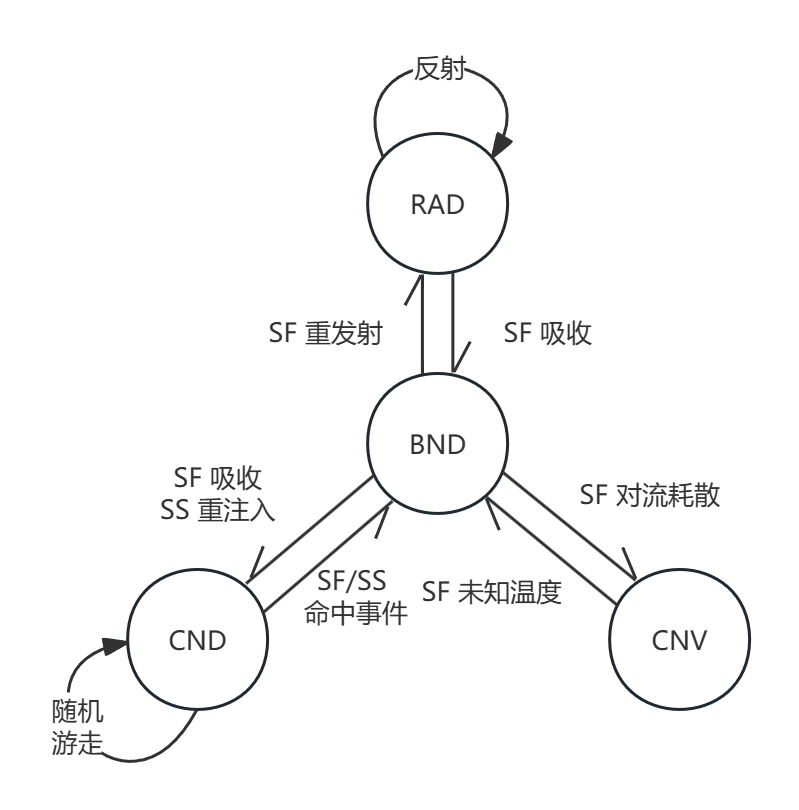
\includegraphics[width=1.0\textwidth]{Figures/Coupled_Path/CoupledPath.png}
  \bicaption{多层嵌套场景耦合热输运蒙特卡洛路径示意图}{Schematic of Monte Carlo path propagation in a multi-layer nested coupled heat transport scene}
  \label{fig:coupled_path}

  \small
  场景为二维截面：外部环境~Fluid~A 中放置固体外壳~Solid~A（$\lambda_A$，橙色），
  其内部包含封闭流体腔~Fluid~B（蓝色）和内嵌固体~Solid~B（$\lambda_B$，绿色），
  Solid~B 内进一步嵌套已知温度固体~Solid~C（浅黄色）。
  路径自探测器出发经辐射传播（RAD）命中~Solid~A 外表面（BND~1），
  渗透进入固体后执行传导随机游走（CND）。
  游走过程中的 $\delta$-球面吸附步可命中三类界面，分别展示：
  反射/对流出射至外部环境（BND~4）、
  再发射穿越封闭腔体（BND~2 $\to$ BND~3）、
  固-固跨壁传导进入相邻固体（BND~5 $\to$ BND~6）。
  图中同时展示全部四种终止条件：
  辐射逃逸（Miss）、对流耗散（Dissipation）、时间回溯（Time）和已知温度（Known Temperature）。
\end{figure}

本节将递归求解器的隐式调用栈状态等价转换为显式有限状态机（FSM）——任何有限递归调用图均可通过将函数返回地址显式化为状态枚举、调用栈局部变量显式化为结构体字段来完成此变换，这是算法等价变换的基本方法。基于细粒度状态机的耦合热路径计算过程可在任意几何查询阶段将完整路径状态持久化至外部结构体并完成挂起，待查询结果到达后从中断点无损恢复执行。以下逐模块展开各物理过程的 FSM 状态组设计，每个模块遵循"物理方程 $\to$ 蒙特卡洛求解步骤 $\to$ 几何查询需求 $\to$ FSM 状态产出"的统一范式。

\subsubsection{辐射传播模块（RAD）：渲染方程驱动的多次弹射}

辐射传播段（RAD）是耦合路径的"外层骨架"：路径从红外探测器出发，在透明流体中沿直线传播，反复在固体表面弹射，直至被吸收或射线未命中任何几何体（Miss）。其物理基础是灰体漫射表面假设下渲染方程（式~\eqref{eq:rendering}）的简化形式——路径追踪对其作 Neumann 级数展开，得到辐射温度的无偏估计量：路径从 $\mathbf{x}$ 沿 $\boldsymbol{\omega}$ 出发，经若干次弹射最终到达固体终止点 $\mathbf{x}_\Gamma$ 的表面温度之期望值。蒙特卡洛逐次采样的弹射规则为：命中表面后以概率 $\varepsilon$ 吸收（终止弹射段），以概率 $(1-\varepsilon)$ 按余弦分布 $\boldsymbol{\omega}' \sim (\boldsymbol{\omega}' \cdot \hat{n})/\pi$ 漫反射继续弹射；若射线未命中任何几何体（Miss），路径终止于预设的环境辐射温度 $\theta_{R,\text{env}}$。

RAD 模块每次弹射产生 1 个 RT 查询（射线最近命中），是全部 FSM 物理模块中结构最简单的。命中后的处理逻辑为：Miss 时以 $\theta_{R,\text{env}}$ 终止路径；命中 Dirichlet 边界时以已知温度直接终止；命中温度待求面时以 $\varepsilon$ 概率吸收、$(1-\varepsilon)$ 概率反射继续弹射。

\textbf{RAD 与 BND 的管理边界}：上述 $\varepsilon$-吸收/$(1-\varepsilon)$-反射是渲染方程 Neumann 展开中的截断采样，本质上属于 RAD 弹射循环的一部分——它决定弹射是否继续。当吸收事件发生后（RAD 弹射段终止），路径转入 BND 模块执行界面处的三模态能量分配（$P_\text{cond}/P_\text{conv}/P_\text{rad}$），决定后续进入 CND、CNV 还是开启新一段 RAD 弹射。因此，RAD 的"吸收出口"即是 BND 的"入口"，两者边界在 $\varepsilon$-吸收决策完成之时。

\begin{figure}[htbp]
  \centering
  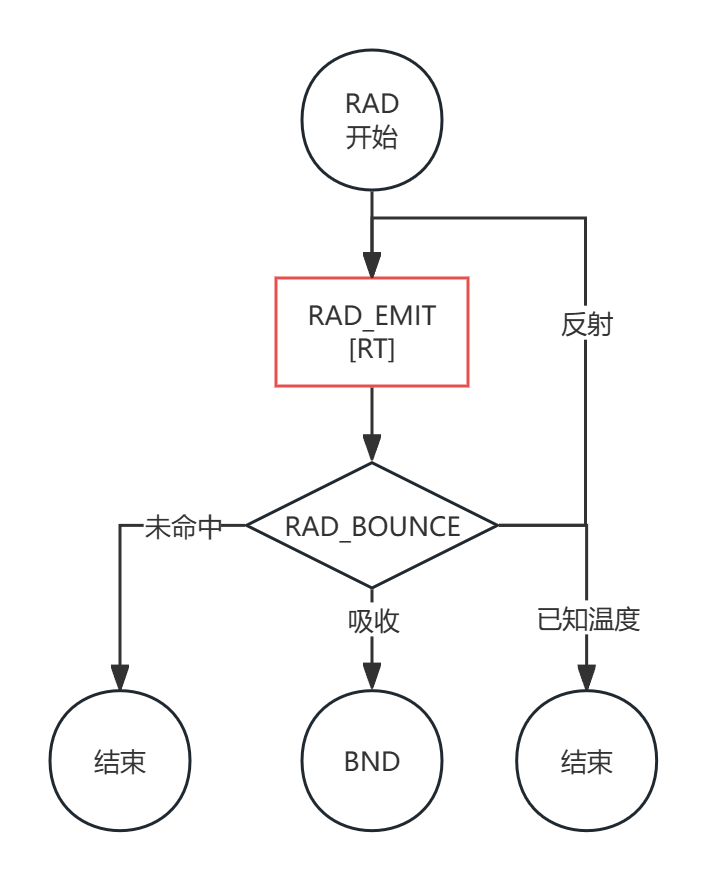
\includegraphics[width=0.5\textwidth]{Figures/FSM_RAD/FSM_RAD.png}
  \bicaption{RAD 辐射传播模块的状态转移图}{FSM state transition diagram of the RAD radiative transport module}
  \label{fig:fsm-rad}

  \small
  圆圈节点为模块入口/出口及终止条件，红色边框方形为含 RT 查询的挂起点，
  菱形为分支决策状态。路径从探测器或 BND 辐射出射进入 RAD，
  经余弦采样弹射循环，以 $\varepsilon$ 概率吸收（转入 BND）或射线逃逸终止。
\end{figure}

\subsubsection{固体传导模块（CND）：扩散方程驱动的球面随机游走}

路径经 BND 模块以传导概率 $P_\text{cond}$ 渗入固体内部后，传播机制从直线辐射切换为球面随机游走——对应图~\ref{fig:coupled_path} 中路径从 BND~1 事件后在 Solid~A 壁体中执行的 CND 折线步进段。球面随机游走求解固体内瞬态扩散方程\cite{batiCouplingConductionConvection2023}：
\begin{equation}
  \frac{\partial \theta_S}{\partial t} = \alpha \Delta \theta_S
  \label{eq:cnd-diffusion}
\end{equation}
其中 $\alpha = k/(\rho c)$ 为热扩散率，$\theta_S$ 为固体温度场。其蒙特卡洛求解由如下估计量驱动：
\begin{equation}
  \theta_S(\mathbf{x} - \delta\hat{n}) = E\bigl[\theta_S(\mathbf{x}_\text{WoS})\bigr]
  \label{eq:cnd-wos-estimator}
\end{equation}
即在固体边界面内侧 $\delta$-偏移处的温度，等于从该点出发的球面随机游走到达边界时温度的期望值。每步将游走粒子投射到球面上的随机位置，球半径由几何或物理参数确定；当粒子到达固体边界时，路径回到 BND 模块开始新一轮界面耦合分叉。实现中存在两种球面游走方案：

\textit{Walk-on-$\delta$-Sphere（$\delta$-球面游走）}使用固定步长参数 $\delta$ 替代最近面距离作为球面半径\cite{batiCouplingConductionConvection2023}。每步采样均匀球面方向 $\boldsymbol{\Omega}$，沿 $+\boldsymbol{\Omega}$ 和 $-\boldsymbol{\Omega}$ 两方向各追踪一条射线（RT 查询），取命中距离 $s^+$、$s^-$ 与 $\delta$ 的最小值作为实际步长：
\begin{equation}
  \tilde{\delta} = \min(\delta,\,s^+,\,s^-)
  \label{eq:cnd-ds-step}
\end{equation}
粒子跳至 $\mathbf{x} + \tilde{\delta}\,\boldsymbol{\Omega}$，随后以 ENC 查询验证新位置的腔体归属。若跳跃后位置进入 $\varepsilon$-壳层（$\tilde{\delta}$-球面吸附至边界），则路径转入 BND 模块——对应图~\ref{fig:coupled_path} 中 CND 游走段的三个出射分支（BND~2、BND~4、BND~5 分别命中固-流内表面、固-流外表面和固-固接触面）；否则进行瞬态时间回溯采样后继续下一步游走。每步产生 1 个 RT 查询（双向射线对批量提交为一次查询）和 1 个 ENC 查询（位置验证）。

\textit{Walk-on-Sphere（经典 WoS 游走）}以最近面投影距离（CP 查询）作为球面半径，在远离边界处收敛性更优（对数收敛 vs $\delta$-球的固定步长）。每步首先执行 CP 查询获取最近面距离 $d_\text{wos}$：若 $d_\text{wos} \leq \varepsilon_\text{shell}(\delta)$，粒子吸附至边界并转入 BND；否则在 $d_\text{wos}$ 半径球面上均匀采样跳跃方向。跳跃后执行第二次 CP 查询验证新位置的最近面距离（扩散位置合法性检查）：若验证失败（新位置处于几何非凸区域），以 RT 查询发射回退射线修正位置。每步产生 2 个 CP 查询（步长估计 $+$ 位置验证）和至多 1 个条件性 RT 查询（仅在验证失败时触发）。

两种方案在实现中并存，由场景参数控制选择策略。

\textit{瞬态时间回溯}嵌入上述两种游走方案每步循环的尾部。按指数分布采样向后时间跳跃 $T_{b,\text{cond}}$，其特征时间为：
\begin{equation}
  \tau_\text{cond} = \frac{\rho c \tilde{\delta}^2}{6k}
  \label{eq:cnd-tau}
\end{equation}
若时间倒退至仿真初始时刻 $t_I$，路径以已知初始温度终止——对应图~\ref{fig:coupled_path} 中的 Done(Time) 终止条件；否则继续下一步游走。此逻辑为确定性计算，不产生额外查询。

\textbf{模块出口}：CND 路径在游走步到达固体边界时转入 BND 模块。如图~\ref{fig:coupled_path} 所示，同一条传导游走路径因命中不同性质的边界面而触发截然不同的后续物理机制——BND~4（固-流外表面，辐射反弹或对流终止）、BND~2（固-流内表面，再发射穿越封闭腔体）、BND~5（固-固接触面，按导热系数比跨壁传导）——由 BND 模块统一处理。

\begin{figure}[htbp]
  \centering
  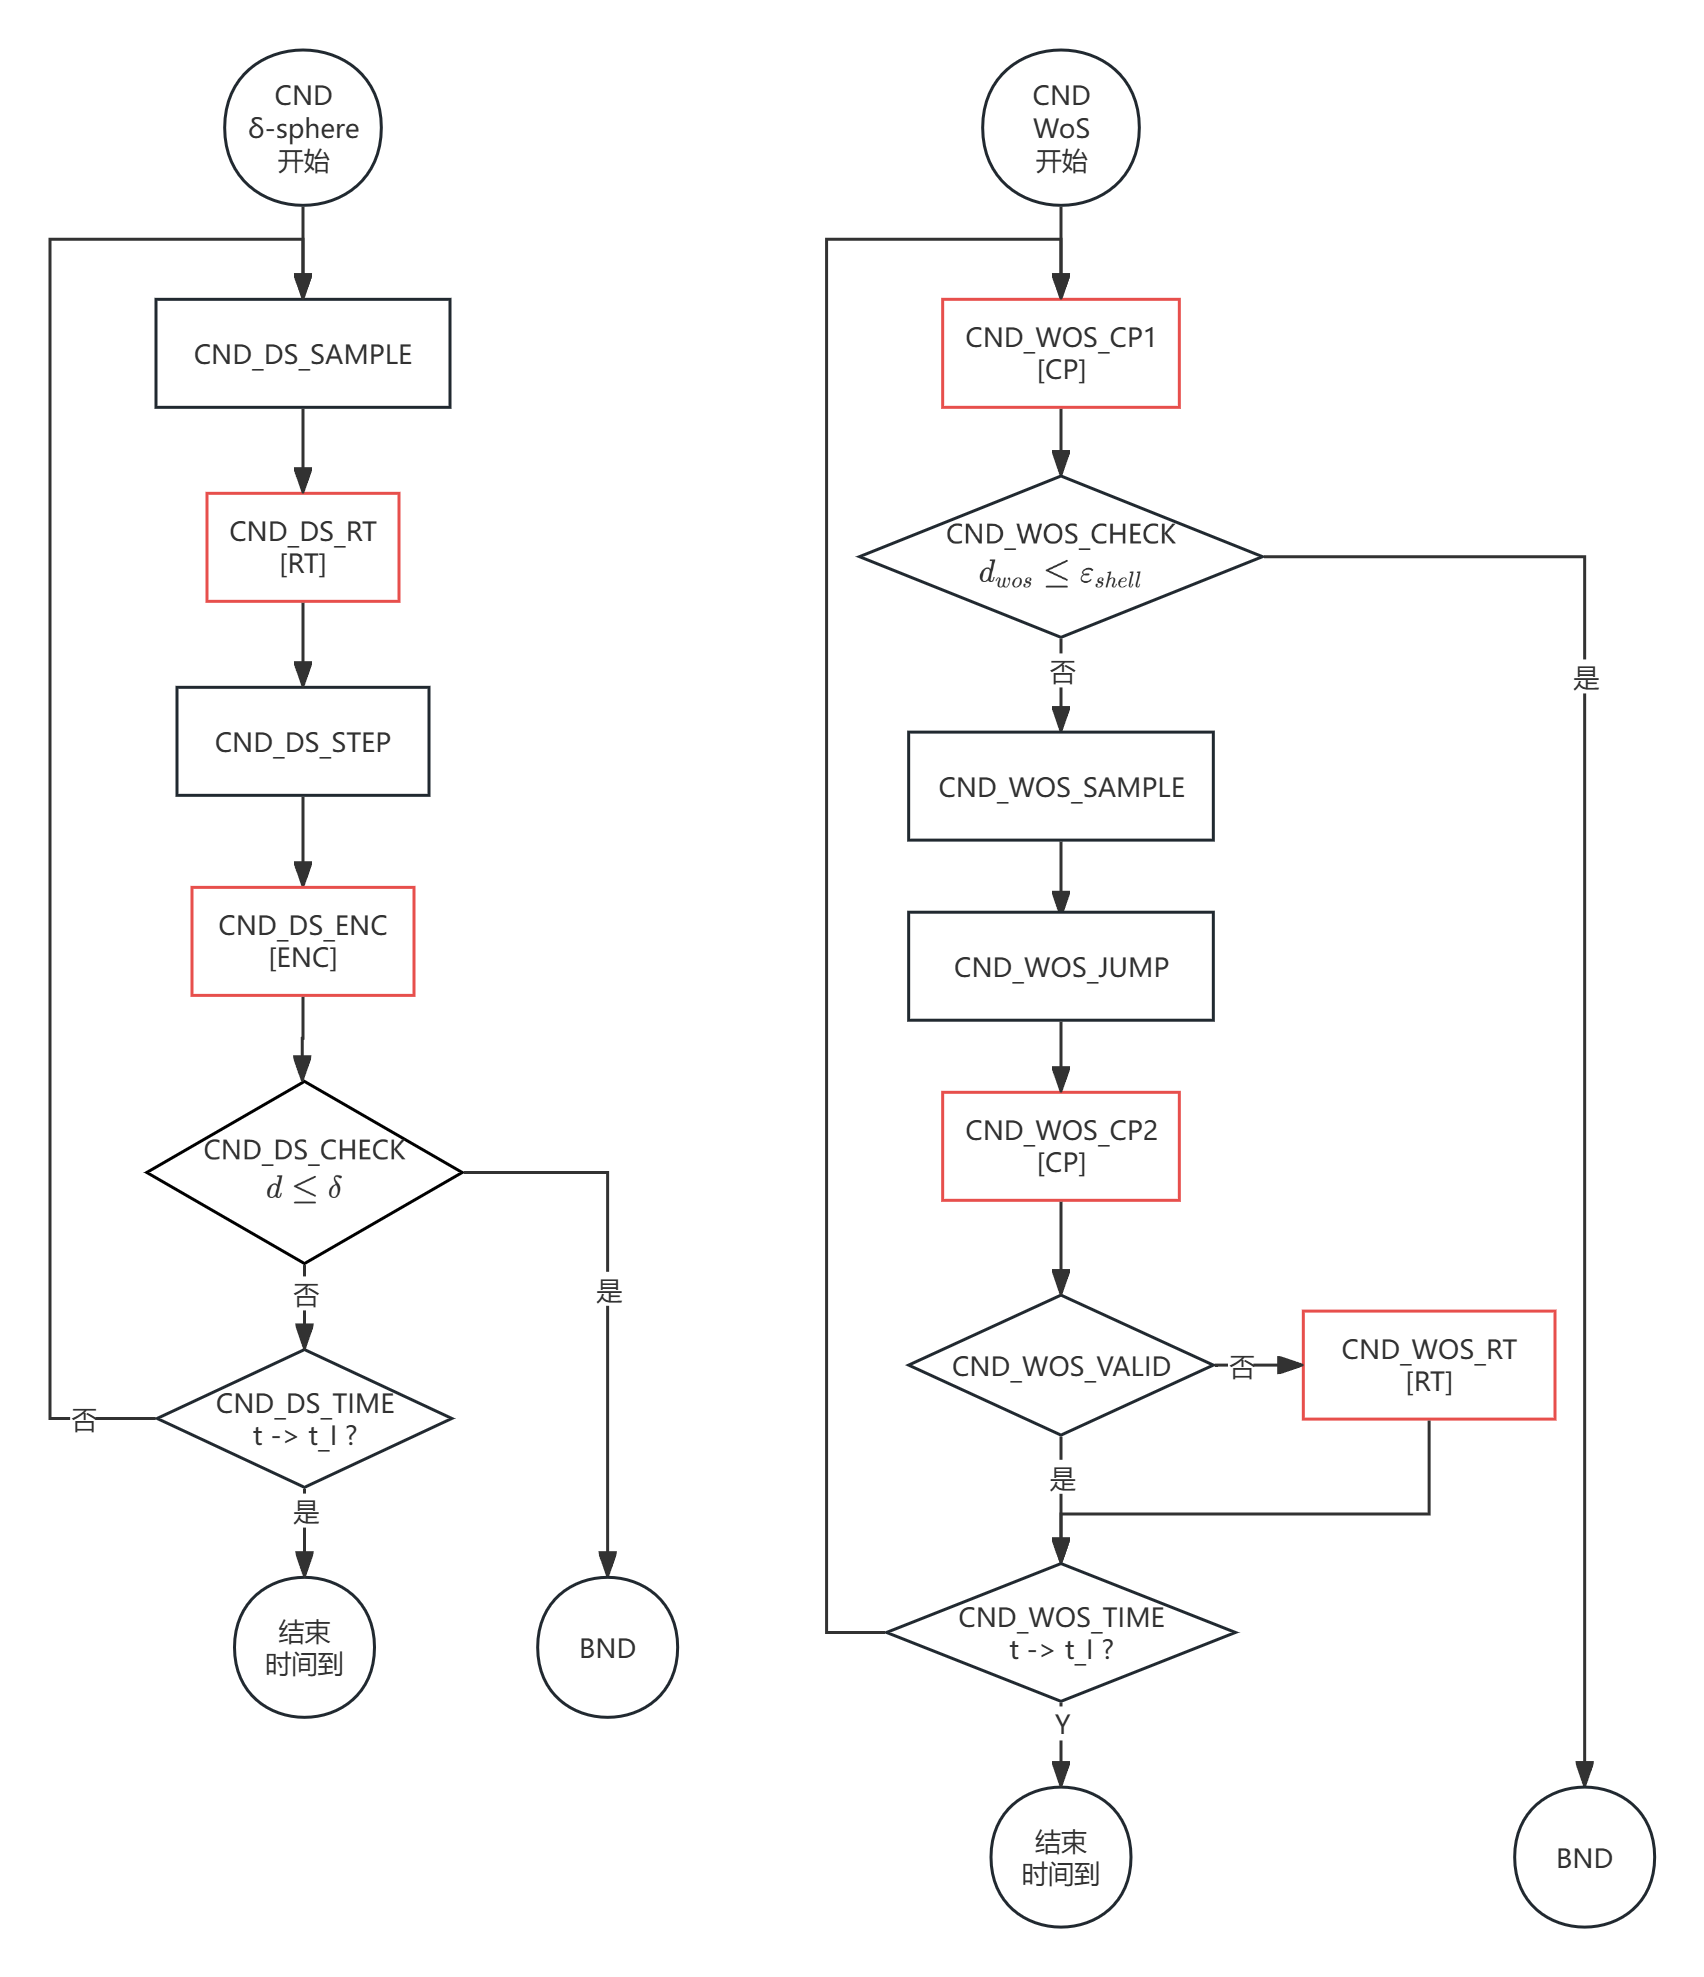
\includegraphics[width=0.7\textwidth]{Figures/FSM_CND/FSM_CND.png}
  \bicaption{CND 固体传导模块的状态转移图}{FSM state transition diagram of the CND solid conduction module}
  \label{fig:fsm-cnd}

  \small
  左侧为 $\delta$-球面游走方案（5 个状态），右侧为经典 WoS 游走方案（8 个状态），
  虚线方框分别包围两种游走方案。圆圈节点为模块入口/出口及终止条件，
  红色边框方形为含几何查询的挂起点（RT/CP/ENC），方形为线性计算状态，菱形为分支决策状态。
\end{figure}

\subsubsection{对流换热模块（CNV）：流体温度的边界采样}

当 BND 模块以对流概率 $P_\text{conv}$ 选择进入对流模式时，路径需获取当前封闭腔体的流体温度 $\theta_F$。\cite{batiCouplingConductionConvection2023} 框架假设完全混合流体（腔体内等温），$\theta_F$ 等于该腔体壁面固体温度的 $h(\mathbf{x})$-加权平均：
\begin{equation}
  \theta_F = E\bigl[\theta_S(\mathbf{X}_S)\bigr], \quad
  \mathbf{X}_S \sim \frac{h(\mathbf{x})}{\int_S h\,\mathrm{d}x}
  \label{eq:cnv-fluid-temp}
\end{equation}
蒙特卡洛采样将此期望估计为：在腔体边界面上按 $h(\mathbf{x})$ 成比例采样一个位置 $\mathbf{X}_S$，读取该处固体温度 $\theta_S(\mathbf{X}_S)$。若该位置温度已知（Dirichlet 边界），路径以 $\theta_F = \theta_S(\mathbf{X}_S)$ 终止——对应图~\ref{fig:coupled_path} 中 BND~4 出射分支的对流耗散终止 Done(Dissipation)；若温度未知，路径在 $\mathbf{X}_S$ 处再次触发 BND 事件，继续分叉求解。瞬态对流在腔体温度采样前引入指数分布的向后时间跳跃 $T_{b,\text{conv}}$，其特征时间为：
\begin{equation}
  \tau_\text{conv} = \frac{\rho c V}{hS}
  \label{eq:cnv-tau}
\end{equation}
其中 $V$ 为腔体体积，$S$ 为腔体壁面面积。若时间倒退至初始时刻 $t_I$，路径以已知初始流体温度终止。

CNV 模块的 FSM 结构包含 1 个 RT 查询，位于模块入口处的腔体几何边界探针射线——该射线确认路径所在腔体的几何边界范围，为后续按 $h(\mathbf{x})$ 采样壁面位置提供几何基础。边界采样本身为确定性计算，不产生额外查询。

\textbf{模块出口}：采样位置 $\mathbf{X}_S$ 处温度已知时路径终止；温度未知时回到 BND 模块继续耦合分叉。CNV 是全部传输模块中 FSM 结构最简洁的：4 个状态、1 个查询，反映了完全混合假设下对流模型的物理简洁性。

\begin{figure}[htbp]
  \centering
  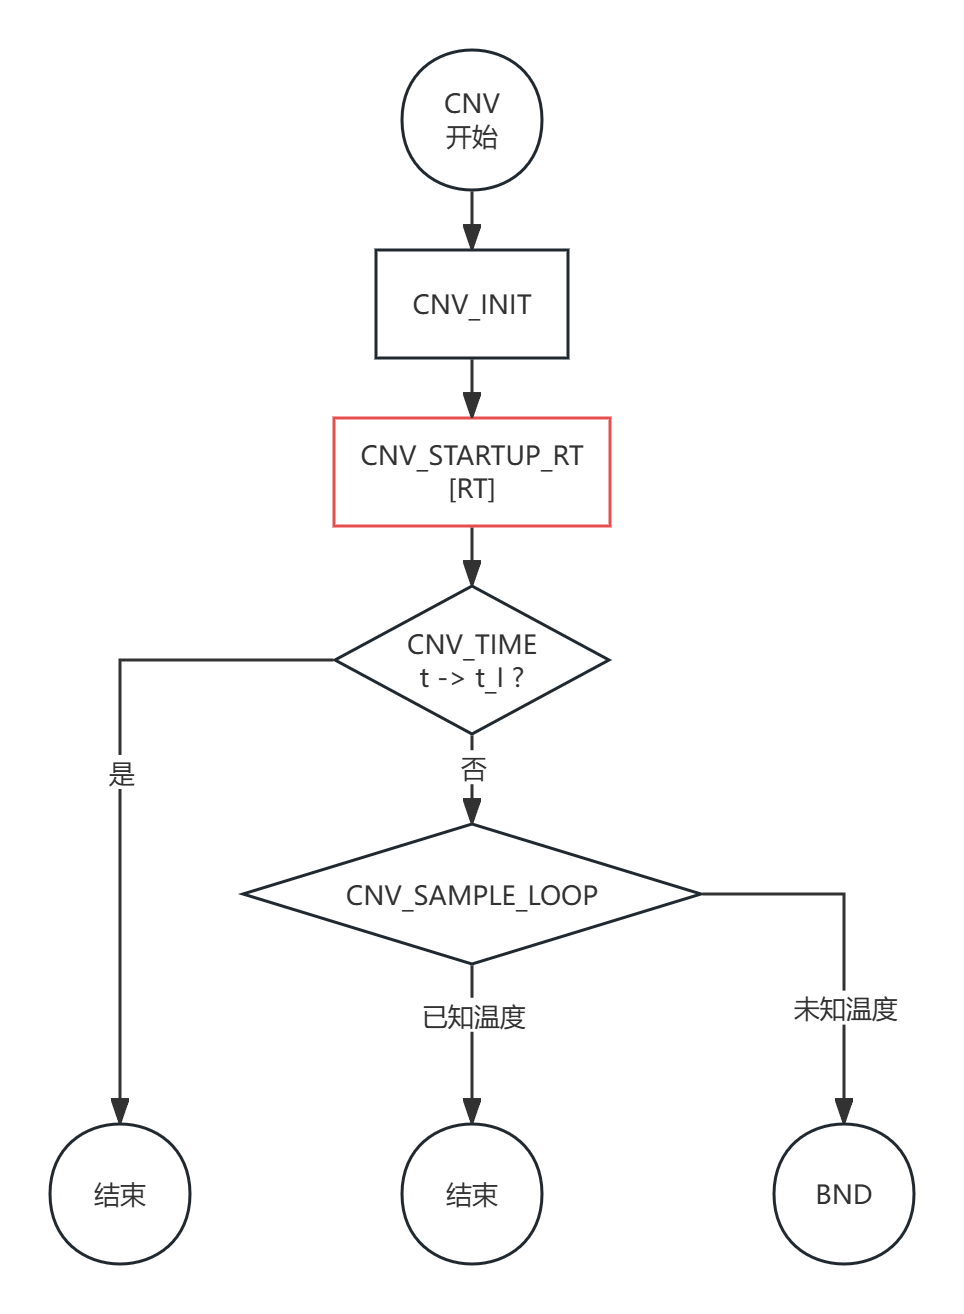
\includegraphics[width=0.4\textwidth]{Figures/FSM_CNV/FSM_CNV.png}
  \bicaption{CNV 对流换热模块的状态转移图}{FSM state transition diagram of the CNV convective heat transfer module}
  \label{fig:fsm-cnv}

  \small
  4 个状态，1 个 RT 查询。圆圈节点为模块入口/出口及终止条件，
  红色边框方形为含 RT 查询的挂起点，方形为线性计算状态，菱形为分支决策状态。
\end{figure}

\subsubsection{界面耦合模块（BND）：能量通量连续性驱动的多模态分叉}

界面耦合模块是整个 FSM 中状态数最多、分叉结构最复杂的部分。物理上，界面是辐射、传导、对流三种热传递模式交汇的核心节点——路径在界面处根据能量守恒的概率分叉决定进入何种传输模式继续前进。前文已分别介绍了 RAD、CND、CNV 三个传输模块的 FSM 结构，本段落展示 BND 如何作为三者的汇聚枢纽，在不同类型的界面处产生多模态分叉与状态回环。

BND 模块的物理总纲是界面能量守恒方程\cite{batiCouplingConductionConvection2023}：在任何固-流界面处，固体侧传导热通量等于流体侧对流通量与辐射通量之和：$\varphi_\text{cond}[\theta] = \varphi_\text{conv}[\theta] + \varphi_\text{rad}[L_\lambda]$。\ref{sec:coupled_framework} 已将此方程改写为概率期望形式（式~\eqref{eq:interface_temp}），界面温度由传导、对流、辐射三种模式的概率加权和表示，三个概率 $P_\text{cond}$、$P_\text{conv}$、$P_\text{rad}$ 由式~\eqref{eq:interface_probs} 给出。路径在界面处按上述概率随机选择进入 CND、CNV 或 RAD 模块——对应图~\ref{fig:coupled_path} 中各 BND 事件节点的扇形概率分支。

实际场景中界面类型多样，FSM 首先经过一个界面分发状态根据界面类型（固-流 / 固-固 / 外部环境）和温度可知性进行分流。下文按界面复杂度递增展开各子模块。

\textit{腔体归属查询（ENC）——界面参数查找的前置步骤}。固-流或固-固界面的物理参数（$\varepsilon$、$k$、$h$）绑定于封闭腔体（enclosure）。如图~\ref{fig:coupled_path} 所示的多层嵌套场景中，Solid~A 的外表面属于 Enc~A 而内表面属于 Enc~B，同一固体的不同面对应不同腔体参数集。路径到达界面后必须首先确定所属腔体才能查找正确的物理系数。腔体归属判定采用 6-ray 轴对齐投票方案：沿 $\pm x$、$\pm y$、$\pm z$ 六方向发射射线，根据命中面片的腔体标注投票确定归属；投票不一致时以随机方向回退射线补充。该过程产生 3 个 ENC 查询（BVH 最邻近定位、6-ray 主投票查询、歧义回退查询）。归属结果写入路径状态，后续全部 BND 子模块依赖此值读取正确物理参数。

\textit{固-流界面（SF）——三模态耦合与 null-collision}。当路径经传导游走到达固-流界面（对应图~\ref{fig:coupled_path} 中 BND~2、BND~4 类事件），或从辐射传播段被吸收后首次进入固体（BND~1），执行式~\eqref{eq:interface_temp} 的三模态概率分叉。FSM 子流程依次为：(1) $\delta$-重注入采样——沿界面法线内侧发射 RT 查询确定传导注入候选位置 $\mathbf{x} - \delta\hat{n}$；(2) 三概率 $P_\text{cond}/P_\text{conv}/P_\text{rad}$ 计算与模式调度——以 Russian Roulette 采样转移目标，传导分支进入 CND 模块、对流分支进入 CNV 模块。辐射分支的处理涉及式~\eqref{eq:null_collision} 所述的 null-collision 机制在界面耦合中的应用（\cite{batiCouplingConductionConvection2023} 6.3）：由于 $P_\text{rad}$ 含 $h_R = 4\sigma\varepsilon\theta_\text{ref}^3$，当参考温度 $\theta_\text{ref}$ 不准确时三概率之和偏离 1；为此设上界 $\hat{h}_R$ 使 $P_\text{rad}^\text{ub}$ 始终合法，采样辐射方向后发射 RT 查询获取子路径辐射温度 $\theta_R$，计算实际 $h_R$ 并以 $h_R/\hat{h}_R$ 概率接受（true collision），否则以 null collision 判定回到分叉状态重新采样。这一 null-collision 循环在 FSM 中对应 PENDING $\to$ 恢复 $\to$ 条件判断 $\to$ 回到 PENDING 的状态回边，与 RAD 弹射循环的 FSM 化方法完全同构。固-流界面子模块共产生 2 个 RT 查询（重注入射线 $+$ null-collision 辐射子路径射线）。图~\ref{fig:coupled_path} 中 BND~1 处的扇形分支即展示了 $P_\text{cond}$（渗入 Solid~A 启动 CND）、$P_\text{rad}$（漫反射回 Fluid~A 继续 RAD）和 $P_\text{conv}$（对流温度终止 $\theta_{F,A}$）三个出射方向。

\textit{PicardN 高阶迭代——递归子路径}。高温差场景中 $h_R$ 对温度强依赖，Picard-1 单轮线性化不足以收敛（\cite{batiCouplingConductionConvection2023} 6.3.3）。具体而言，$h_R = 4\sigma\varepsilon\theta_\text{ref}^3$ 是对 Stefan-Boltzmann 四次方律 $\sigma\varepsilon\theta^4$ 在参考温度 $\theta_\text{ref}$ 处的一阶 Taylor 线性化\cite{batiCouplingConductionConvection2023}。当界面两侧温差较小时，$\theta_\text{ref}$ 的选取误差对 $h_R$ 影响有限，Picard-1 的单轮 null-collision 采样即可收敛；而当温差显著时，$h_R \propto \theta_\text{ref}^3$ 的立方依赖使任何初始估计的偏差被放大，需通过多轮子路径采样逐步收紧 $\theta_\text{ref}$ 估计。PicardN 在界面处递归展开子路径树：每层展开至多 $N_\text{branch}$ 条完整耦合子路径（实现中 $\leq 6$ 条），递归深度可达 3 层。其 FSM 化的核心挑战在于将嵌套递归压平为显式栈：\texttt{path\_state} 中预分配固定深度递归栈（\texttt{path\_sfn\_data}，3 层，约 3.7\,KB/路径），以栈指针模拟展开与回退。子路径复用主 FSM 全部状态集（RAD/BND/CND/CNV）和挂起/恢复机制，不引入新的设计维度——仅增加栈管理字段。PicardN 的 6 个细粒度 FSM 状态及其查询与前述各模块的 FSM 化方法完全同构，不再逐一展开。

\textit{固-固界面（SS）——双侧导热注入}。当传导游走路径到达两个相邻固体子部件的接触面（对应图~\ref{fig:coupled_path} 中 BND~5: Solid~A $\leftrightarrow$ Solid~B），物理方程为式~\eqref{eq:ss_interface} 的传导通量连续性条件\cite{batiCouplingConductionConvection2023}。路径以 $P_{\text{cond},1}$ 概率选择注入固体 1 侧、以 $P_{\text{cond},2}$ 概率注入固体 2 侧的 $\delta$ 偏移处，继续传导游走。固-固界面不涉及辐射和对流模态（两侧均为不透明固体），分叉结构远简于固-流界面——仅为二元导热概率选择。FSM 子流程中，双侧各以 2 条射线（法线 $+$ 偏移修正）确定 $\delta$-注入候选位置（共 4 条 RT 批量提交），随后以 1 个 ENC 查询验证候选位置腔体归属，最终按概率选侧后进入 CND 模块。图~\ref{fig:coupled_path} 中 BND~5 注入 Solid~B 后路径继续游走，经 BND~6 最终终止于已知温度 Done(Known Temperature)。

\textit{外部环境边界（EXT）——净辐射通量子流程}。当路径到达与开放辐射环境交界的外部边界（而非封闭腔体内表面），需计算该表面从外部环境接收的净辐射通量（太阳直射 $+$ 天空漫射 $-$ 自发射），对应 \cite{batiCouplingConductionConvection2023} Eq.\,7 中 $\varphi_\text{rad}$ 的外部环境部分。蒙特卡洛子流程分三步有序执行：(1) 沿太阳方向发射阴影射线测试直射遮挡（RT 查询）；(2) 在天空半球按分布采样漫射方向（RT 查询）；(3) 对漫射命中方向发射遮挡验证射线（RT 查询）。三步严格有序，每步依赖前一步结果，须分配独立查询。该子模块共产生 3 个 RT 查询，是 BND 子模块中状态数最多的（8 个细粒度状态），反映了外部环境辐射场的多源（直射 $+$ 漫射）特征。

\begin{sidewaysfigure}
  \centering
  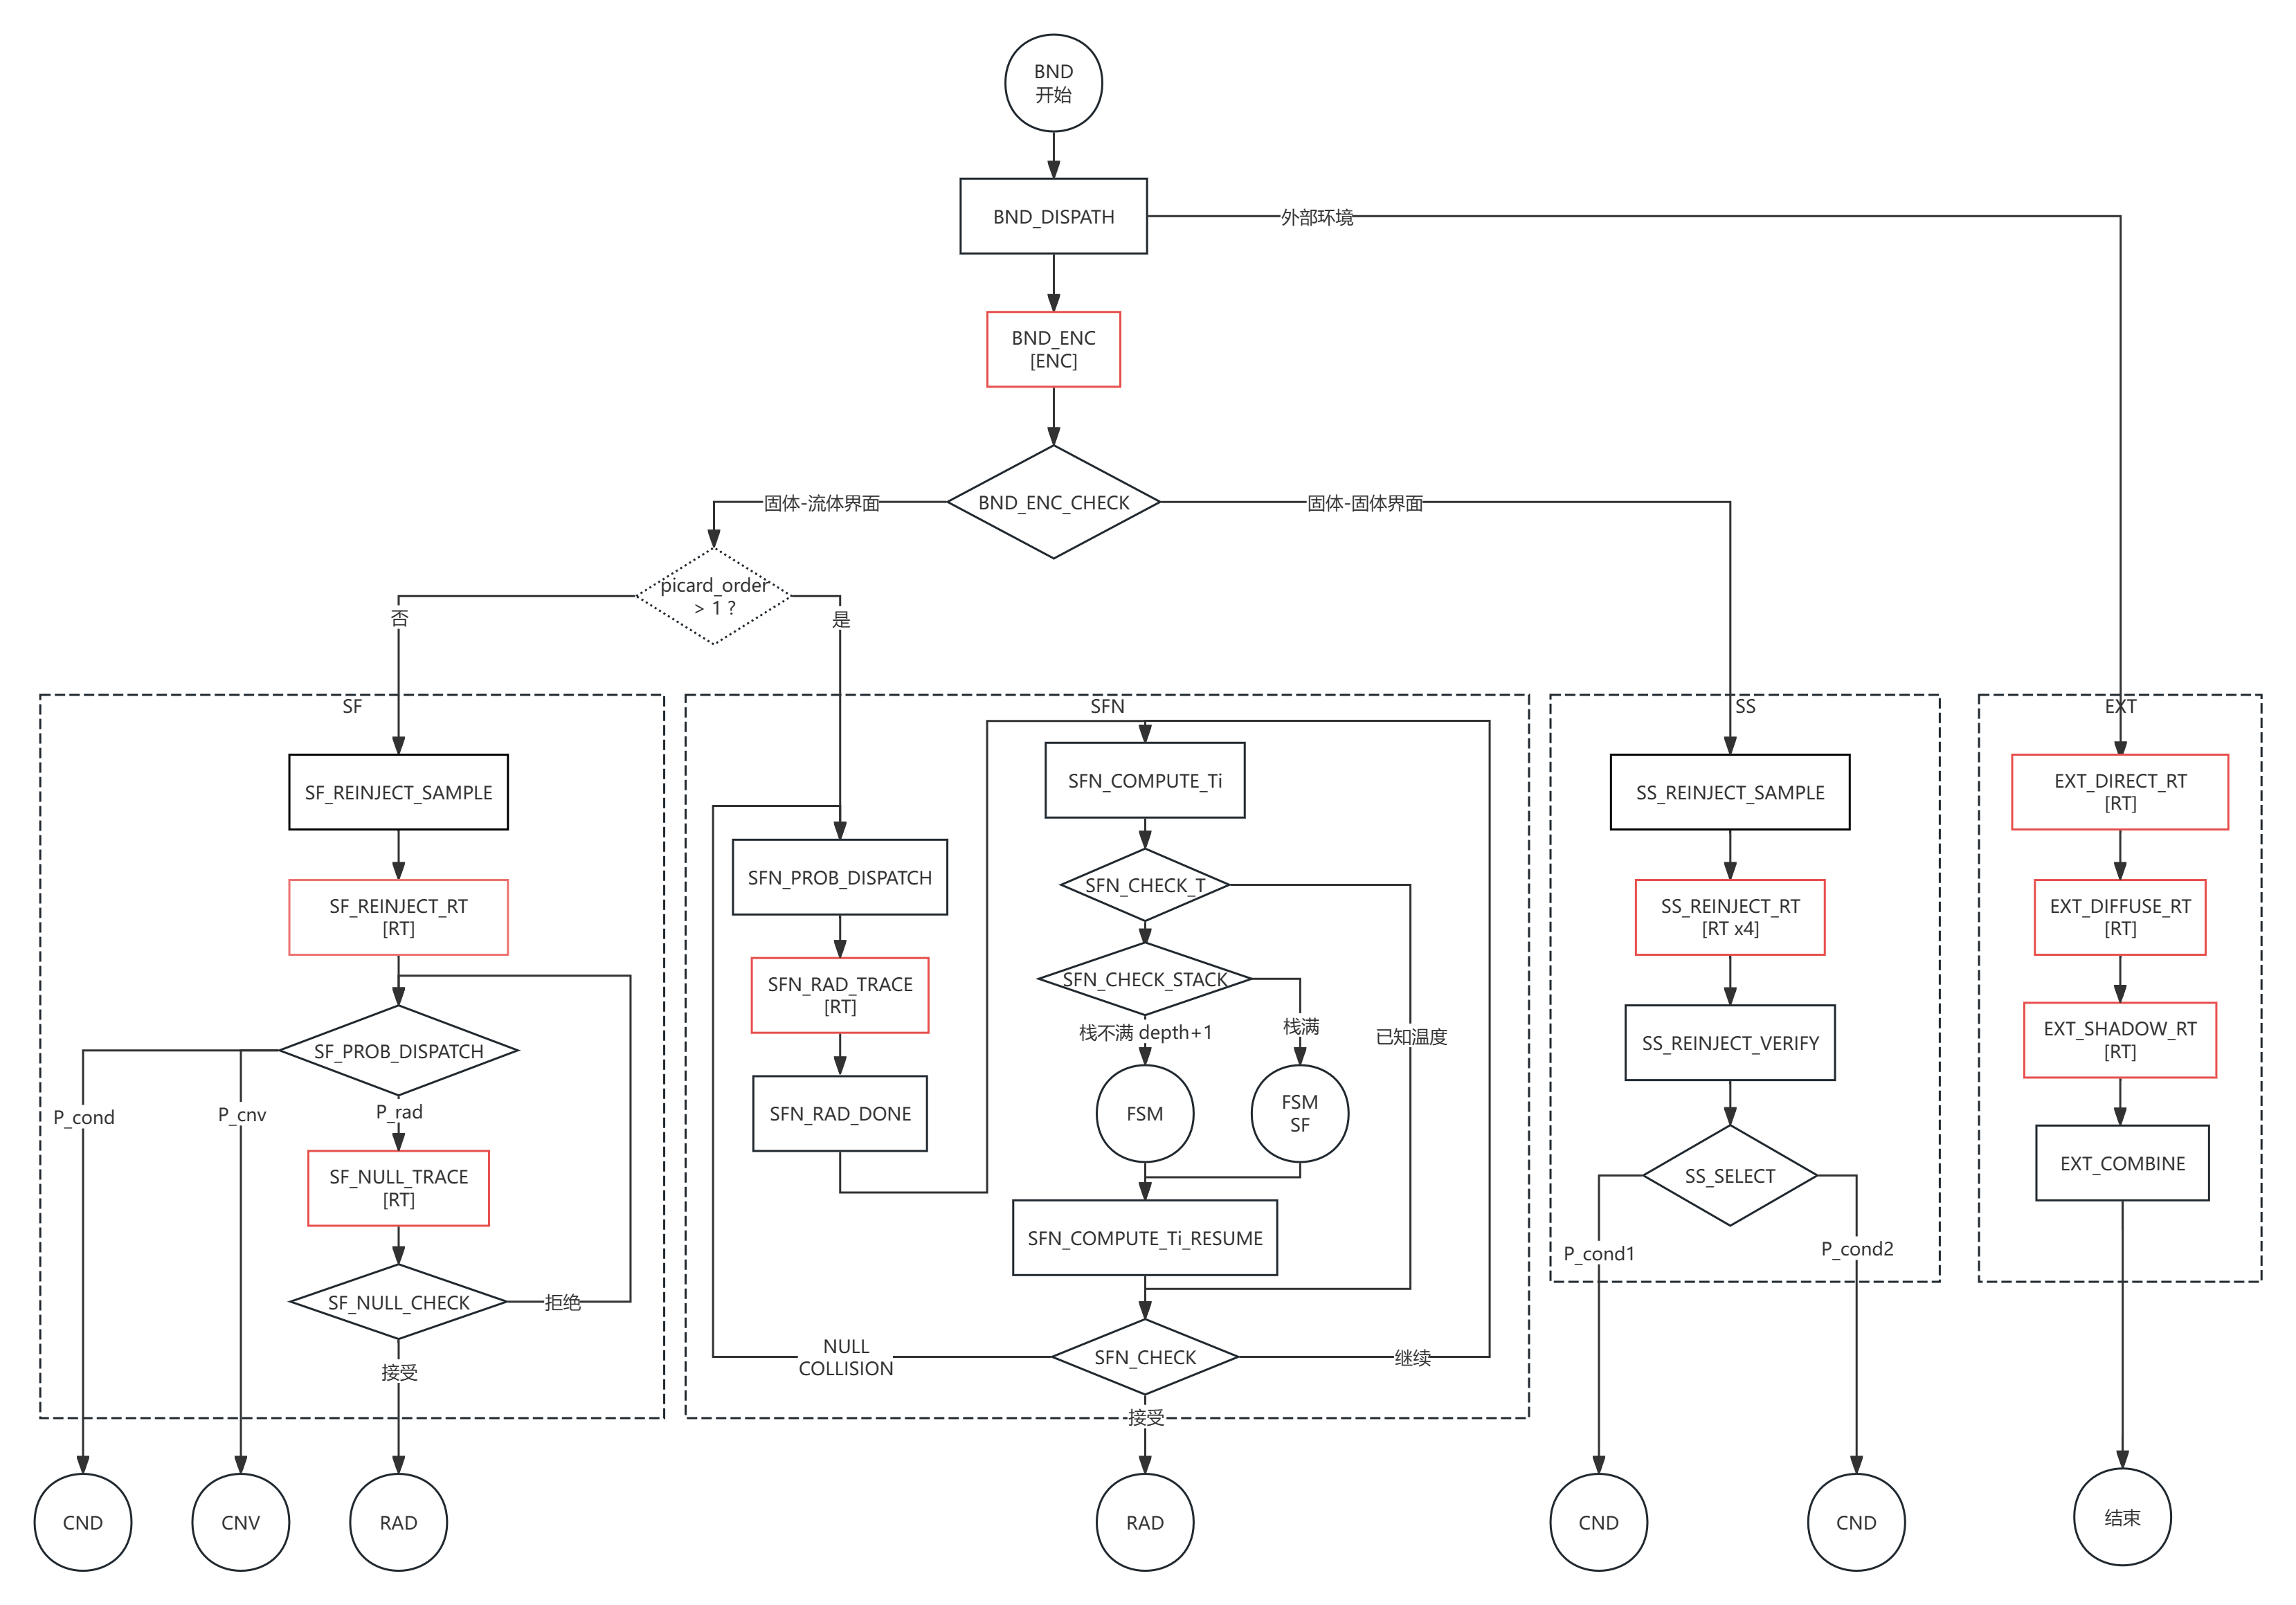
\includegraphics[width=0.9\textheight]{Figures/FSM_BND/FSM_BND.png}
  \bicaption{BND 界面耦合模块的分层状态转移图}{Hierarchical FSM state transition diagram of the BND interface coupling module}
  \label{fig:fsm-bnd}

  \small
  虚线方框包围 ENC、SF、SFN、SS、EXT 五个子模块。圆圈节点为模块入口/出口及终止条件，
  红色边框方形为含几何查询的挂起点（RT/ENC），方形为线性计算状态，菱形为分支决策状态。
  红色虚线回边标记 null-collision 循环，蓝色虚线标记 SFN 子路径迭代与栈递归。
\end{sidewaysfigure}

\subsubsection{完整 FSM 综合：模块组装与路径生命周期}

以上四个物理过程模块（RAD、CND、CNV）及其界面耦合枢纽（BND，含 ENC、SF、SFN、SS、EXT 五个子模块）共同构成耦合热输运路径的完整 FSM。组装方式由物理耦合关系唯一决定：路径从探测器出发经 RAD 弹射到达固体表面后进入 BND，BND 按界面类型和概率将路径分发至 CND（传导游走）、CNV（对流采样）或继续 RAD（辐射再发射）；CND 和 CNV 完成后再次返回 BND，形成 $\text{BND} \rightleftharpoons \text{CND/CNV/RAD}$ 的反复交替，直至路径终止于已知温度、初始时刻、环境辐射或俄罗斯轮盘赌截断四类条件之一。\cref{fig:coupled_path_meta} 已从粗粒度视角展示了这一模块间流转结构。

表~\ref{tab:module-summary} 汇总了各模块的状态数与几何查询需求。FSM 共包含 59 个细粒度状态，分属上述模块——其数量不是任意设计的结果，而是物理耦合复杂度的自然投影：3 种热传递模式 $\times$ 多种界面拓扑（固-流、固-固、外部环境）$\times$ 非线性耦合迭代（null-collision、PicardN）$\times$ 瞬态时间维度 $\times$ 实际几何复杂度（嵌套腔体），每种组合需要独立的查询通道。路径长度是场景物理参数（导热率、发射率、腔体尺度）的函数：最短可仅 2 步（RAD 直达 Dirichlet 边界终止），最长可达数千步（深 PicardN 递归 $+$ 长传导游走 $+$ 多次界面往返）。

\begin{table}[htbp]
  \centering
  \bicaption{各物理模块的 FSM 状态数与几何查询汇总}{Summary of FSM state counts and geometric queries by physical module}
  \label{tab:module-summary}
  \small
  \begin{tabular}{lccccc}
    \toprule
    物理模块 & 物理方程来源 & 状态数 & RT & ENC & CP \\
    \midrule
    RAD 辐射传播 & Bati Eq.\,6/19 & 2 & 1 & — & — \\
    BND-ENC 腔体归属 & 工程需求 & 3 & — & 3 & — \\
    BND-SF（Picard-1） & Bati Eq.\,23, 6.3 & 5 & 2 & dep & — \\
    BND-SFN（PicardN） & Bati 6.3.3 & 6 & 1+ & dep & — \\
    BND-SS 固-固界面 & Bati Eq.\,26 & 3 & 4 & dep & — \\
    BND-EXT 外部环境 & Bati Eq.\,7 & 8 & 3 & — & — \\
    CND-DS（$\delta$-Sphere） & Bati 4.2 & 5 & 2/步 & dep & — \\
    CND-WoS（Walk-on-Sphere） & Muller 1956 & 8 & 1 & — & 2 \\
    CNV 对流换热 & Bati Eq.\,28 & 4 & 1 & dep & — \\
    \midrule
    \textbf{合计} & — & \textbf{59} & \textbf{14 点} & \textbf{3 点} & \textbf{2 点} \\
    \bottomrule
  \end{tabular}

  \vspace{4pt}
  {\raggedright\footnotesize 注："dep"表示该模块依赖 ENC 查询结果（由 BND-ENC 子模块提供），但不直接产生 ENC 查询。"2/步"表示每个游走步产生 2 个 RT 查询。"1+"表示 PicardN 子路径复用主 FSM 各模块的 RT 查询，此处仅计入 PicardN 独有的辐射子路径射线查询。\par}
\end{table}

全部 19 个查询在本文的 Wavefront 实现中均为同构查询：RT、ENC、CP 三类查询均已后端化（第四章详述），共享同一批量提交接口。Wavefront 主循环无需区分查询类型，统一收集、统一提交、统一恢复，调度逻辑因此大幅简化。

值得说明的是，Wavefront 求解器下多条路径的随机数消耗顺序与递归求解器不同（递归求解器逐路径串行消耗，Wavefront 求解器按批次交错消耗），但各路径持有独立的 per-path 计数器基随机数生成器（CBRNG）密鑰，路径内部随机序列相互独立，消耗顺序的差异不影响蒙特卡洛估计量的统计无偏性。

\subsection{Wavefront 执行模型}
\label{subsec:wf-model}

3.3.1 将递归求解器等价改造为显式路径状态机（FSM），使单条路径在任意几何查询节点均可将完整中间状态持久化至外部结构体 \texttt{path\_state}，并在查询结果回填后无损恢复执行。至此，单条路径的可挂起性已经建立。

然而，可挂起性本身尚不构成批量化的充分条件。3.3.1 的 FSM 仅定义了单条路径的状态与转移规则；如何组织多条路径的并发调度——何时挂起、何时恢复、如何将分散在不同路径中的查询请求聚合为一个连续批次——尚未涉及。形式化地，设 $N$ 条路径同时处于活跃状态，每条路径在其生命周期内经历若干次几何查询挂起；在任一时刻，各路径处于 59 个 FSM 状态中的某一个，其中处于 \textsc{Pending} 状态的路径各自持有一条待执行的查询请求。问题可表述为：设计一种调度策略，使得 (1) 每轮迭代中所有 \textsc{Pending} 路径的查询请求被提取并聚合为连续缓冲区，统一提交至查询后端批量执行；(2) 执行结果回填至各路径的 \texttt{path\_state} 后，路径从挂起点恢复继续推进。

Laine 等人\cite{laineMegakernelsConsideredHarmful2013}在 GPU 路径追踪中提出的 Wavefront 执行模型为上述问题提供了成熟的架构范式（第 2.3 节已介绍其基本原理）。其核心思想是：以固定容量的路径池维护所有活跃路径的持久化状态，主循环在每轮迭代中完成查询结果回填、路径推进、已完成路径收割、空闲槽位补充与新查询请求收集，最终将该轮收集的全部查询批量提交至后端——如此往复，直至全部采样任务完成。本节将 Wavefront 范式应用于 3.3.1 的耦合热输运 FSM，设计具体的主循环结构。

\subsubsection{主循环结构}
Wavefront 求解器以固定容量的路径池（Path Pool）$\mathcal{P}[0..N_\text{pool}-1]$ 为核心数据结构，每个槽位存储一个 \texttt{path\_state} 结构体及其调度阶段标记 \texttt{phase}。\texttt{phase} 在调度层面取四种值：\textsc{Pending}（持有待执行查询，等待后端返回结果）、\textsc{Ready}（结果已回填，可继续推进 FSM）、\textsc{Done}（求解完成，待收割）、\textsc{Free}（空闲槽位）。主循环重复执行六个阶段直至全部像素采样完成，如算法~\ref{alg:wf-main-loop} 所示。

\begin{algorithm}
\caption{Wavefront 耦合热输运求解器主循环}
\label{alg:wf-main-loop}
\begin{algorithmic}[1]
\REQUIRE pixel task queue $\mathcal{Q}$, path pool $\mathcal{P}[0..N_\text{pool}-1]$, query backend $\mathcal{B}$
\ENSURE per-pixel temperature estimates $\hat{T}[\cdot]$
\WHILE{$\mathcal{Q}$ non-empty \textbf{or} $n_\text{active} > 0$}
  \STATE \textsc{DistributeResults}($\mathcal{P}$, $\mathcal{H}$) \COMMENT{Phase 1: 查询结果回填}
  \STATE \textsc{AdvancePaths}($\mathcal{P}$) \COMMENT{Phase 2: 路径状态推进}
  \STATE \textsc{HarvestDone}($\mathcal{P}$, $\hat{T}$) \COMMENT{Phase 3: 完成路径收割}
  \STATE \textsc{RefillSlots}($\mathcal{P}$, $\mathcal{Q}$) \COMMENT{Phase 4: 空闲槽位补充}
  \STATE \textsc{CollectQueries}($\mathcal{P}$, $\mathcal{R}$) \COMMENT{Phase 5: 查询请求提取}
  \STATE $\mathcal{B}$.\texttt{submit}($\mathcal{R}$) \COMMENT{Phase 6: 批量提交至查询后端}
\ENDWHILE
\end{algorithmic}
\end{algorithm}

该六阶段序列与本文实现的实际执行顺序一一对应，构成 Wavefront 求解器的最小调度循环——每个阶段承担单一职责，各阶段间以路径池 $\mathcal{P}$ 与请求/结果缓冲区（$\mathcal{R}$/$\mathcal{H}$）为共享数据进行隐式通信。以下算法~\ref{alg:wf-p1}--\ref{alg:wf-p5} 分别给出 Phase 1--5 各阶段的操作伪代码（Phase 6 \texttt{submit} 为后端接口调用，不展开）。

\textbf{Phase 1: \textsc{DistributeResults}}（算法~\ref{alg:wf-p1}）。将上轮后端返回的查询结果写回各路径。遍历路径池，对每条处于 \textsc{Pending} 状态的路径，将结果缓冲区 $\mathcal{H}$ 中对应条目的命中位置、法线、距离等字段写入其 \texttt{path\_state}，并将调度标记切换为 \textsc{Ready}，表示该路径可继续推进。

\begin{algorithm}[htbp]
\caption{\textsc{DistributeResults} — 查询结果回填}
\label{alg:wf-p1}
\begin{algorithmic}[1]
\FOR{$i = 0$ \textbf{to} $N_\text{pool}-1$}
  \IF{$\mathcal{P}[i].\texttt{phase} = \textsc{Pending}$}
    \STATE write $\mathcal{H}[\texttt{owner}^{-1}(i)]$ (hit position, normal, distance, $\ldots$) into $\mathcal{P}[i].\texttt{state}$
    \STATE $\mathcal{P}[i].\texttt{phase} \leftarrow \textsc{Ready}$
  \ENDIF
\ENDFOR
\end{algorithmic}
\end{algorithm}

\textbf{Phase 2: \textsc{AdvancePaths}}（算法~\ref{alg:wf-p2}）。推进所有 \textsc{Ready} 路径。对每条 \textsc{Ready} 路径反复调用 3.3.1 的 \texttt{fsm\_step}，执行 FSM 状态转移直至路径再次到达查询挂起点（\textsc{Pending}）或求解完成（\textsc{Done}）。两次挂起之间可能跨越多个 FSM 状态——例如从 BND 概率分叉到 CND WoS 步进再到下一挂起射线——均在此阶段内完成。

此处存在一个关键细节：3.3.1 的 PicardN 子模块通过显式递归栈将父路径"分裂"为子路径——子路径复用与普通路径完全同构的 FSM 状态集与推进/收割管线，这一同构性是 Wavefront 批量处理的内在要求。然而，当子路径完成求解到达 \textsc{Done} 时，若不加拦截，\textsc{HarvestDone} 将直接回收该槽位，连同父路径的递归栈帧一起被清除。为此，\textsc{AdvancePaths} 在每次 \texttt{fsm\_step} 后插入一项递归子路径拦截检查：若路径到达 \textsc{Done} 且其 PicardN 递归栈深度 $d_\text{sfn} > 0$（即当前路径是某层递归的子路径而非顶层路径），则将 FSM 状态重置为 \texttt{SFN\_COMPUTE\_Ti\_RESUME}、调度标记回退为 \textsc{Ready}，使推进循环继续执行。被拦截的路径随后在 FSM 内部完成栈弹出与父层上下文恢复，对求解器而言只需一行栈深度判断，全部递归复杂度被封装在 FSM 状态转移逻辑中。

\begin{algorithm}[htbp]
\caption{\textsc{AdvancePaths} — 路径状态推进}
\label{alg:wf-p2}
\begin{algorithmic}[1]
\FOR{$i = 0$ \textbf{to} $N_\text{pool}-1$}
  \IF{$\mathcal{P}[i].\texttt{phase} = \textsc{Ready}$}
    \REPEAT
      \STATE \texttt{fsm\_step}($\mathcal{P}[i]$) \COMMENT{执行一次 FSM 状态转移（3.3.1）}
      \IF{$\mathcal{P}[i].\texttt{phase} = \textsc{Done}$ \textbf{and} $\mathcal{P}[i].\texttt{state}.d_\text{sfn} > 0$}
        \STATE $\mathcal{P}[i].\texttt{state}.\texttt{fsm} \leftarrow \texttt{SFN\_COMPUTE\_Ti\_RESUME}$ \COMMENT{拦截递归子路径}
        \STATE $\mathcal{P}[i].\texttt{phase} \leftarrow \textsc{Ready}$ \COMMENT{继续推进而非收割}
      \ENDIF
    \UNTIL{$\mathcal{P}[i].\texttt{phase} \in \{\textsc{Pending}, \textsc{Done}\}$}
  \ENDIF
\ENDFOR
\end{algorithmic}
\end{algorithm}

\textbf{Phase 3: \textsc{HarvestDone}}（算法~\ref{alg:wf-p3}）。收割已完成路径。对每条 \textsc{Done} 路径，将其携带的估计值累加至对应像素的温度估计 $\hat{T}$，然后将槽位标记为 \textsc{Free}，供后续 \textsc{RefillSlots} 补入新路径。

\begin{algorithm}[htbp]
\caption{\textsc{HarvestDone} — 完成路径收割}
\label{alg:wf-p3}
\begin{algorithmic}[1]
\FOR{$i = 0$ \textbf{to} $N_\text{pool}-1$}
  \IF{$\mathcal{P}[i].\texttt{phase} = \textsc{Done}$}
    \STATE $\hat{T}[\mathcal{P}[i].\texttt{pixel}]$ += $\mathcal{P}[i].\texttt{value}$; \quad $n_\text{active} \leftarrow n_\text{active} - 1$
    \STATE $\mathcal{P}[i].\texttt{phase} \leftarrow \textsc{Free}$
  \ENDIF
\ENDFOR
\end{algorithmic}
\end{algorithm}

\textbf{Phase 4: \textsc{RefillSlots}}（算法~\ref{alg:wf-p4}）。从像素任务队列 $\mathcal{Q}$ 中取出新采样任务填入空闲槽位。每条新路径初始化探测器位置、初始方向与 CBRNG 密钥，并在 \texttt{state} 中准备初始查询（首条射线），\texttt{phase} 直接置为 \textsc{Pending}。

\begin{algorithm}[htbp]
\caption{\textsc{RefillSlots} — 空闲槽位补充}
\label{alg:wf-p4}
\begin{algorithmic}[1]
\FOR{$i = 0$ \textbf{to} $N_\text{pool}-1$}
  \IF{$\mathcal{P}[i].\texttt{phase} = \textsc{Free}$ \textbf{and} $\mathcal{Q}$ non-empty}
    \STATE $(\text{pixel}, \text{sample\_id}) \leftarrow \mathcal{Q}.\texttt{dequeue}()$
    \STATE initialize $\mathcal{P}[i]$: detector position, initial direction, CBRNG key
    \STATE prepare startup query (initial ray) in $\mathcal{P}[i].\texttt{state}$
    \STATE $\mathcal{P}[i].\texttt{phase} \leftarrow \textsc{Pending}$; \quad $n_\text{active} \leftarrow n_\text{active} + 1$
  \ENDIF
\ENDFOR
\end{algorithmic}
\end{algorithm}

\textbf{Phase 5: \textsc{CollectQueries}}（算法~\ref{alg:wf-p5}）。遍历路径池，从所有 \textsc{Pending} 路径的 \texttt{path\_state} 中提取查询参数（射线起点、方向、查询类型标识等），紧凑追加至请求缓冲区 $\mathcal{R}$，同时记录每条查询到其所属路径槽位的映射 \texttt{owner}，供下轮 \textsc{DistributeResults} 定位回填目标。由于 3.3.1 的同构查询设计——RT、ENC、CP 三类查询共享同一后端提交接口——\textsc{CollectQueries} 无需按查询类型分流，统一追加即可。

\begin{algorithm}[htbp]
\caption{\textsc{CollectQueries} — 查询请求提取}
\label{alg:wf-p5}
\begin{algorithmic}[1]
\STATE $n_\text{queries} \leftarrow 0$
\FOR{$i = 0$ \textbf{to} $N_\text{pool}-1$}
  \IF{$\mathcal{P}[i].\texttt{phase} = \textsc{Pending}$}
    \STATE extract query type, ray origin, direction from $\mathcal{P}[i].\texttt{state}$
    \STATE $\mathcal{R}[n_\text{queries}] \leftarrow$ query; \quad $\texttt{owner}[n_\text{queries}] \leftarrow i$
    \STATE $n_\text{queries} \leftarrow n_\text{queries} + 1$
  \ENDIF
\ENDFOR
\end{algorithmic}
\end{algorithm}

各阶段对路径 \texttt{phase} 标记的操作构成确定性的状态流转环：\textsc{DistributeResults} 将 \textsc{Pending} 转为 \textsc{Ready}（结果已写回，允许推进）；\textsc{AdvancePaths} 将 \textsc{Ready} 推进至 \textsc{Pending}（产生新查询）或 \textsc{Done}（求解完成）；\textsc{HarvestDone} 将 \textsc{Done} 释放为 \textsc{Free}；\textsc{RefillSlots} 将 \textsc{Free} 初始化为 \textsc{Pending}（含初始查询）；\textsc{CollectQueries} 仅读取 \textsc{Pending} 路径的查询参数，不改变状态。因此，任一路径在其生命周期内按如下序列流转：
\begin{equation*}
\textsc{Free} \xrightarrow{\text{Refill}} \textsc{Pending} \xrightarrow{\text{Distribute}} \textsc{Ready} \xrightarrow{\text{Advance}} \cdots \xrightarrow{\text{Advance}} \textsc{Done} \xrightarrow{\text{Harvest}} \textsc{Free}
\end{equation*}

首轮迭代时 \textsc{DistributeResults} 和 \textsc{AdvancePaths} 因无 \textsc{Pending}/\textsc{Ready} 路径而自然空转，\textsc{RefillSlots} 填充路径池后交由 \textsc{CollectQueries} 收集初始查询，调度循环自此进入稳态。

路径池容量 $N_\text{pool}$ 在求解器启动时确定，全部 \texttt{path\_state} 结构体以连续数组分配。路径池运行宏观上分为两个阶段：\textit{填充阶段}——像素任务队列 $\mathcal{Q}$ 尚有未分配任务，每轮 \textsc{RefillSlots} 将空闲槽填满新路径，路径池填充率接近 100\%，提交的查询规模保持在峰值附近；\textit{收尾阶段}——$\mathcal{Q}$ 已空，\textsc{RefillSlots} 无新路径补入，活跃数逐轮递减直至清零。

\textbf{路径优先遍历优化}。算法~\ref{alg:wf-p1}--\ref{alg:wf-p3} 及算法~\ref{alg:wf-p5} 各独立遍历路径池一次（四次线性扫描）。在实现中，本文将此四次扫描融合为单次路径优先（path-centered）遍历——对每条路径连续执行 distribute$\to$advance$\to$harvest/collect 完整序列后才移向下一条路径。该融合确保同一条路径的 \texttt{path\_state} 在被首次加载到缓存行后，后续全部操作均在该缓存行驻留期间完成，显著改善缓存局部性。路径优先遍历不改变各阶段的语义——仅将四次独立扫描合并为一趟，是纯实现层面的优化。

综上，Wavefront 主循环在 \textsc{Collect} 与 \textsc{Distribute} 两阶段之间形成了明确的批量请求/批量响应接口边界：\textsc{Collect} 产出请求缓冲区 $\mathcal{R}$（经 \texttt{submit} 提交至后端），\textsc{Distribute} 消费后端返回的结果缓冲区 $\mathcal{H}$——查询的具体执行过程对状态推进逻辑完全透明。这条接口边界将求解器的计算职责一分为二：状态推进（Phase 1--5，逻辑密集、缓存敏感）与批量查询执行（Phase 6 \texttt{submit}，高吞吐、并发密集）。两类计算需求的分离是 3.3.3 异构架构设计的直接出发点。

\subsection{CPU-GPU 混合执行架构}
\label{subsec:hybrid-arch}

3.3.2 的 Wavefront 主循环在 \textsc{Collect} 与 \textsc{Distribute} 之间形成了明确的批量接口边界，将求解器的计算职责分为两个角色：角色 A（状态推进）——运行 distribute、advance、harvest、refill、collect 等逻辑（算法~\ref{alg:wf-p1}--\ref{alg:wf-p5}），频繁随机读写 \texttt{path\_state} 数组；角色 B（批量查询执行）——接受请求缓冲区 $\mathcal{R}$ 中数万条查询请求，返回结果缓冲区 $\mathcal{H}$。两角色在数据流上的解耦是 Wavefront 执行模型的直接产物。本节在此基础上，根据两类计算的硬件资源需求特征，设计 CPU-GPU 混合执行架构与异步调度机制。

\subsubsection{架构选型与接口设计}

3.3.2 的 Wavefront 批量接口将求解器的计算职责分离为状态推进（角色 A：算法~\ref{alg:wf-p1}--\ref{alg:wf-p5}）与批量查询执行（角色 B：\texttt{submit}）两类独立任务，这两类任务天然适合由 CPU-GPU 异构架构分别承担：角色 A 由 CPU 执行，角色 B 由 GPU 执行。两角色通过一个设备无关的查询接口层交互，接口层定义三个操作原语：
\begin{itemize}[nosep]
  \item \texttt{submit($\mathcal{R}$, $n$)}：将 $n$ 条查询请求提交至后端，异步语义——调用立即返回，后端在独立执行上下文中并行处理。
  \item \texttt{sync()}：等待最近一次 \texttt{submit} 对应的后端计算完成。
  \item \texttt{retrieve($\mathcal{H}$, $n$)}：将 $n$ 条查询结果从后端传输至结果缓冲区 $\mathcal{H}$。
\end{itemize}
接口层将后端的具体执行设备对角色 A 完全屏蔽。请求缓冲区 $\mathcal{R}$ 与结果缓冲区 $\mathcal{H}$ 采用结构体数组（SoA）布局，以连续内存存储同类查询字段，便于后端以对齐方式批量读取。

\textbf{本文选用的后端实例化}：角色 B 由 NVIDIA GPU 承担——三类几何查询的 GPU 批量管线设计（RT 光追管线、CP 最近面投影管线、ENC 腔体归属管线）将在第四章独立展开。本节以下内容聚焦于两角色在异步通信下的调度架构设计。

\subsubsection{Path-Centered 合并遍历}
\label{subsubsec:merge-pass}

\ref{subsec:wf-model} 将角色 A 的单轮工作描述为五个顺序 Phase——Distribute、Advance、Harvest、Refill、Collect——每个 Phase 各自遍历路径池数组。然而在实际落地时，路径池规模为 16\,384\textasciitilde 32\,768 条路径，每条 \texttt{path\_state} 约 3\textasciitilde 4\,KB；整个路径池工作集达 50\textasciitilde 128\,MB，远超典型 CPU 的 LLC 容量（16\textasciitilde 32\,MB）。若各 Phase 依次独立扫描路径池数组，则每轮产生多次完整遍历，每次遍历均将上一 Phase 的热缓存行逐出 LLC，导致大量 LLC miss 开销。

为消除这一缓存压力，实现将四个逐路径 Phase 合并为一次 path-centered 遍历（merged pass）。概念上，循环组织从
\begin{center}
\begin{minipage}{0.42\textwidth}
\begin{algorithmic}[0]
\FOR{\textbf{each} phase $p$ \textbf{in} \{1..5\}}
  \FOR{\textbf{each} path \textbf{in} pool}
    \STATE $p$(path)
  \ENDFOR
\ENDFOR
\end{algorithmic}
\end{minipage}%
\hfill$\Longrightarrow$\hfill%
\begin{minipage}{0.42\textwidth}
\begin{algorithmic}[0]
\FOR{\textbf{each} path \textbf{in} pool}
  \STATE Distribute(path)
  \STATE Advance(path)
  \STATE Harvest(path)
  \STATE Collect(path)
\ENDFOR
\STATE Compact(pool) ; Refill(pool)
\end{algorithmic}
\end{minipage}
\end{center}
右侧结构使每条路径的 \texttt{path\_state} 仅加载一次 L1 缓存行，四个操作在该缓存行仍热时依次完成：
Distribute 写回上一轮光追/CP/ENC 结果并触发对应 step 函数；
Advance（cascade）在无新查询需求的路径上执行内循环推进直至状态机进入 \texttt{needs\_ray}、\texttt{PATH\_DONE} 或 \texttt{PATH\_ERROR}；
Collect 将需要查询的路径的请求写入线程局部缓冲区；
Harvest 收集已完成路径的估计器结果。
遍历结束后，线程局部缓冲区合并至全局请求缓冲区 $\mathcal{R}$。

Refill（空槽填充）与 Compact（活跃索引重建）因涉及路径池级全局状态变更，无法逐路径嵌入，故保留为合并遍历之后的独立阶段。最终角色 A 的单轮 View 处理降为三步：
\[
  \texttt{merged\_pass}(\mathcal{V}) \;\to\; \texttt{compact}(\mathcal{V}) \;\to\; \texttt{refill}(\mathcal{V}) \;\to\; \texttt{submit}(\mathcal{V}.\mathcal{R})
\]
相比原始五次独立扫描，合并遍历将路径池的完整遍历次数从五次降至一次，大幅减少 LLC 换入换出开销，是缩短 $T_A$ 的关键手段。

\subsubsection{单池时序瓶颈与双池 Ping-Pong 调度}

在算法~\ref{alg:wf-main-loop} 的单路径池循环中，角色 A 完成本轮 collect 并调用 \texttt{submit} 后，必须阻塞于 \texttt{sync()} 等待后端返回结果，此间角色 A 完全空闲；反之，角色 A 执行 Phase 1--5 期间后端亦无任务可执行。将两角色的单轮耗时分别记为 $T_A$（Phase 1--5：distribute + advance + harvest + refill + collect）和 $T_B$（submit + 后端执行 + retrieve），则单池循环的每轮墙钟时间为 $T_A + T_B$，两角色的有效利用率均不超过 $\max(T_A, T_B) / (T_A + T_B)$。当角色 B 为 GPU 后端时，$T_B$ 包含 PCIe 传输（H2D + D2H）与 GPU kernel 执行，均可通过异步 DMA 和非阻塞 launch 在独立硬件上下文中执行而不占用 CPU 计算资源——但在单池架构下，角色 A 无法利用这一异步能力，因为当前路径池的状态已提交至后端、结果尚未返回，角色 A 没有可处理的路径。图~\ref{fig:timing-single-pool} 展示了这一串行瓶颈。

\begin{figure}[htbp]
  \centering
  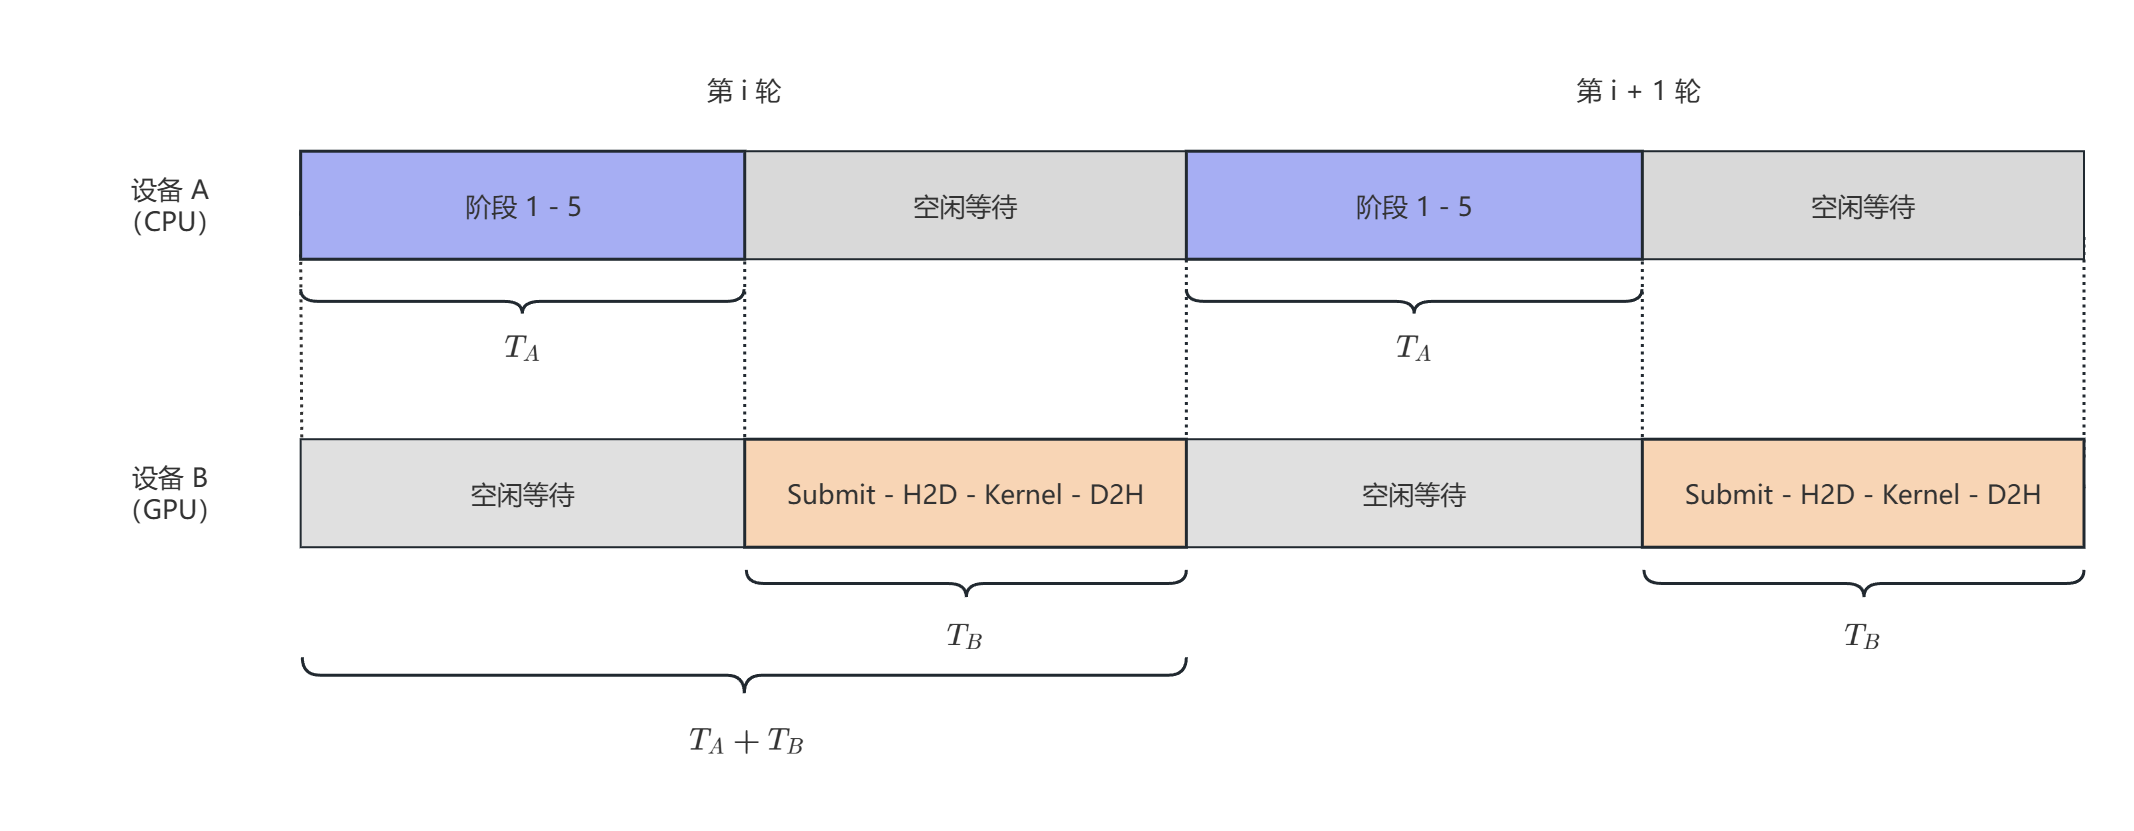
\includegraphics[width=0.90\textwidth]{Figures/Timing_SinglePool/SinglePoolTimeline.png}
  \bicaption{单路径池架构执行时序}{Execution timeline of the single-pool architecture}
  \label{fig:timing-single-pool}

  \small
  上行为角色 A（CPU）时间轴，下行为角色 B（GPU 后端）时间轴。
  角色 A 的工作段（蓝色，Phase 1--5）与角色 B 的工作段（橙色，Submit--H2D--Kernel--D2H）严格串行：角色 A 执行 Phase 1--5 期间角色 B 处于 Idle Waiting（灰色），角色 B 执行批量查询期间角色 A 同样处于 Idle Waiting（灰色）。
  大括号标注各段耗时：$T_A$（角色 A 单轮耗时）、$T_B$（角色 B 单轮耗时），每轮墙钟时间为 $T_A + T_B$，两角色从不同时工作。
\end{figure}

\textbf{双池 Ping-Pong 调度}通过将路径池拆分为两个半独立视图（View $\alpha$、View $\beta$），使两角色的执行时间窗口交错重叠，从根本上消除上述空闲间隙。算法~\ref{alg:pingpong} 展示了双池主循环的核心结构。

\begin{algorithm}
\caption{双池 Ping-Pong 主循环}
\label{alg:pingpong}
\begin{algorithmic}[1]
\REQUIRE path pool views $\mathcal{V}_\alpha$, $\mathcal{V}_\beta$; query backend $\mathcal{B}$
\STATE current $\leftarrow \alpha$; \quad pending $\leftarrow \beta$
\STATE $\mathcal{B}$.\texttt{submit}($\mathcal{V}_\beta.\mathcal{R}$) \COMMENT{bootstrap: pre-submit View $\beta$}
\WHILE{任务未全部完成}
  \STATE $\mathcal{B}$.\texttt{sync}() \COMMENT{等待 View $pending$ 的后端查询完成}
  \STATE $\mathcal{B}$.\texttt{retrieve}($\mathcal{V}_{pending}.\mathcal{H}$) \COMMENT{结果回传至 View $pending$}
  \STATE Phase 1--5 on View $current$ \COMMENT{角色 A: distribute$\to$advance$\to$harvest$\to$refill$\to$collect}
  \STATE $\mathcal{B}$.\texttt{submit}($\mathcal{V}_{current}.\mathcal{R}$) \COMMENT{角色 B 开始执行 View $current$ 批次}
  \STATE swap(current, pending) \COMMENT{视图切换}
\ENDWHILE
\end{algorithmic}
\end{algorithm}

双池调度的时序关键在于：角色 A 处理 View $current$ 的 Phase 1--5（distribute$\to$advance$\to$harvest$\to$refill$\to$collect）时段，与角色 B 执行 View $pending$ 的批量查询在时间上完全重叠。具体而言：角色 A 提交 View $\alpha$ 的批次后立即切换至处理 View $\beta$ 的上一轮结果，此时后端在独立硬件上下文中并行执行 View $\alpha$ 的查询；待角色 A 处理完 View $\beta$ 并提交其新批次时，View $\alpha$ 的结果已就绪，角色 A 可立即取回并切换回处理 View $\alpha$。图~\ref{fig:timing-pingpong} 展示了这一交错执行时序。

\begin{figure}[htbp]
  \centering
  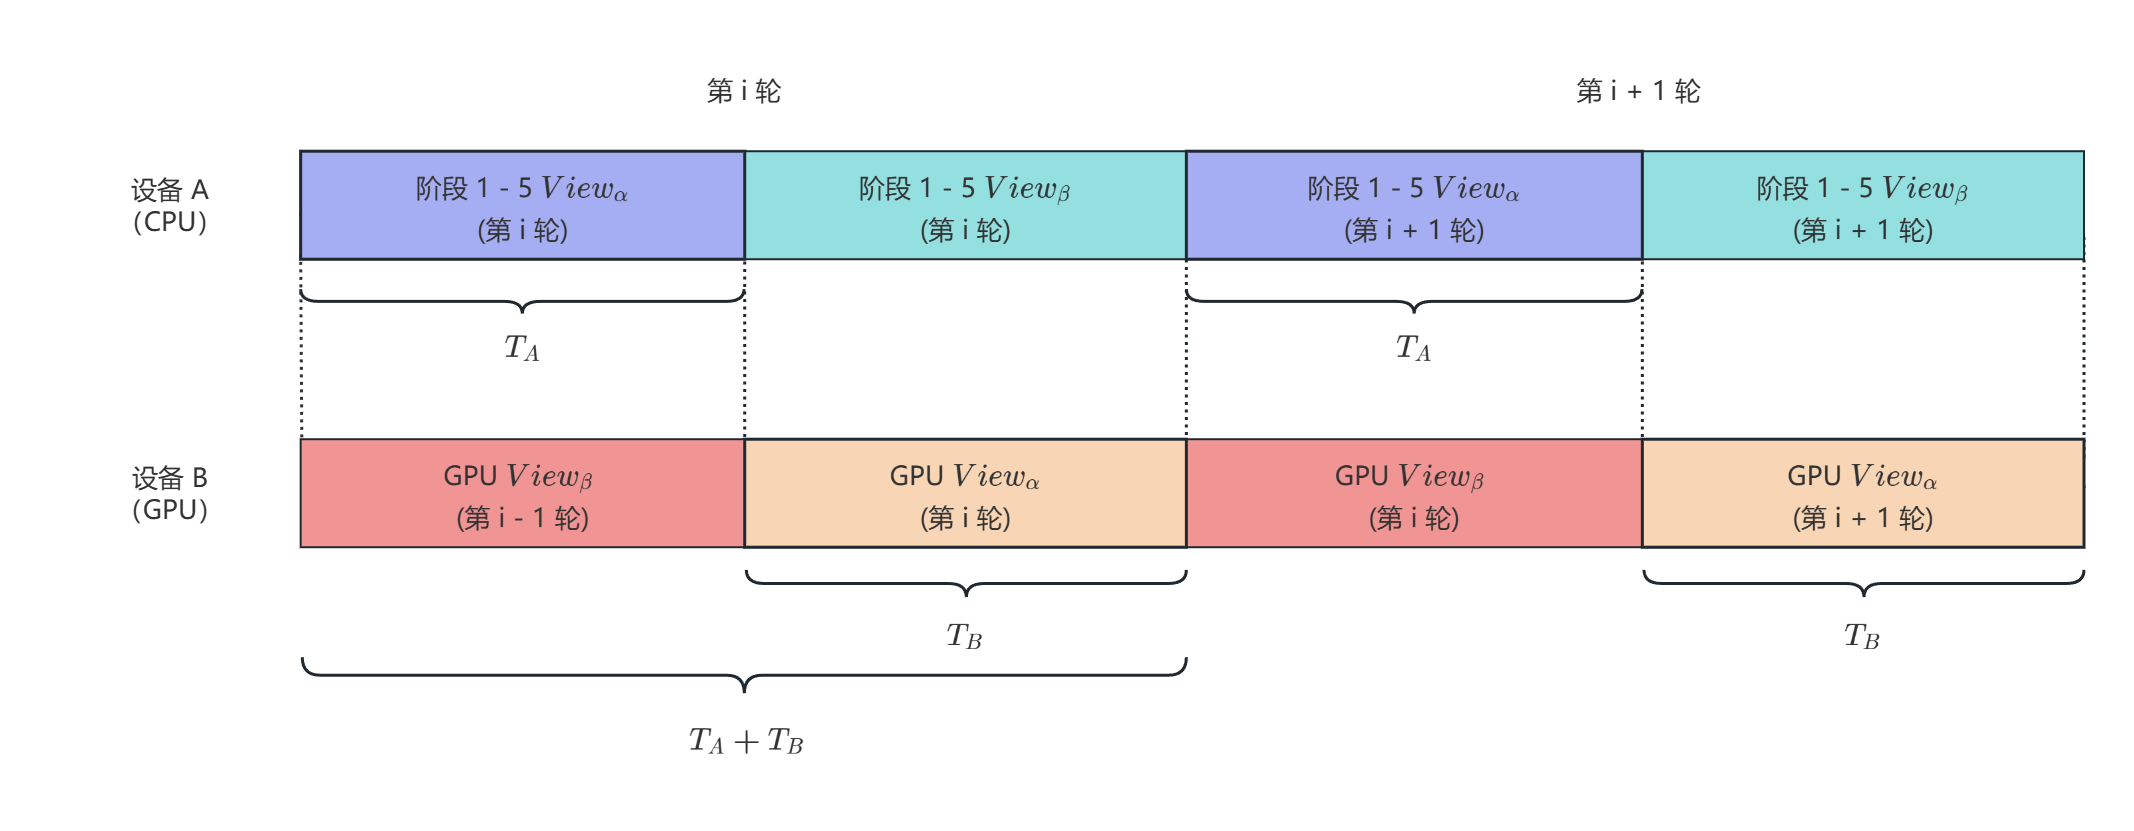
\includegraphics[width=0.90\textwidth]{Figures/Timing_PingPong/DualPoolTimeline.png}
  \bicaption{双池 Ping-Pong 调度执行时序}{Execution timeline of dual-pool Ping-Pong scheduling}
  \label{fig:timing-pingpong}

  \small
  上行为角色 A（CPU）时间轴，下行为角色 B（GPU 后端）时间轴。
  角色 A 的工作段以颜色区分两个 View：View $\alpha$（紫色）与 View $\beta$（青色）交替排列；角色 B 对应地以粉色（GPU View $\beta$）与橙色（GPU View $\alpha$）交替执行批量查询，每段标注所属 Round 编号。
  与图~\ref{fig:timing-single-pool} 对比可见：对任意单个 View 而言，其完整处理周期仍为 $T_A + T_B$（延迟未缩短）；但图~\ref{fig:timing-single-pool} 中两角色的空闲间隙（灰色段）现已被另一 View 的计算任务填充——延迟被隐藏而非缩短。
  大括号标注各段耗时：$T_A$（角色 A 单轮耗时）、$T_B$（角色 B 单轮耗时）；系统吞吐量从单池的每 $(T_A + T_B)$ 完成一个 View 提升至每 $\max(T_A, T_B)$ 完成一个 View，在 $T_A \approx T_B$ 条件下可达约两倍吞吐量。
\end{figure}

需要强调的是，双池调度并不缩短单个 View 的处理延迟——每个 View 从 distribute 到 retrieve 完成仍需经历完整的 $T_A + T_B$。其核心机制在于延迟隐藏：通过引入第二个 View 填充原本闲置的设备时间，使系统吞吐量从单池的每 $(T_A + T_B)$ 完成一个 View 提升至每 $\max(T_A, T_B)$ 完成一个 View。当两角色耗时匹配（$T_A \approx T_B$）时，吞吐量接近单池的两倍。不可避免的同步等待仅发生在两角色耗时不平衡时——当 $T_B > T_A$ 时，角色 A 在 \texttt{sync()} 处等待后端完成；当 $T_A > T_B$ 时，后端在完成本批次后等待角色 A 提交下一批。3.4 的性能分析将报告实测吞吐量提升。

当角色 B 由 GPU 承担时，$T_B$ 进一步分解为三个可与角色 A 部分重叠的子阶段：请求上行传输（H2D，由非阻塞 DMA 执行）、GPU kernel 计算（RT/CP/ENC 三类查询在各自独立的 compute stream 上并行调度，三条流之间无数据依赖）、结果下行传输（D2H，同样由非阻塞 DMA 执行）。H2D 和 D2H 均通过异步 DMA 实现，不占用角色 A 的 CPU 计算资源——这使得即便在 PCIe 带宽受限的条件下，数据传输延迟也可被角色 A 的计算时间所隐藏。

\section{结果与性能评估}

\subsection{实验设置}

本节描述实验环境与评估方法。实验在配备 Intel Core i9-13900K 处理器（8 Performance + 16 Efficiency 核心，P-core 睿频 5.8 GHz）和 NVIDIA GeForce RTX 4090 显卡（Ada Lovelace 架构，16384 CUDA Cores，128 第三代 RT Cores）的工作站上进行，搭配 64 GB DDR5 内存，操作系统为 Windows 11。软件工具链包括 MSVC 19.41（Visual Studio 2022 17.11）、CUDA 12.6、OptiX 8.0 和 NVIDIA 驱动 560.94。Windows 电源计划设置为"高性能"模式以禁用 CPU 频率降档，GPU Boost 保持默认启用（自适应频率）。

每组性能配置运行 3 次，取墙钟时间中位数作为报告值。

测试场景选用 porous（多孔泡沫）场景，包含 13{,}010 个三角面片和多个封闭腔体。该场景材质涵盖高发射率辐射表面（RAD/BND 过程密集）和内部导热体（CND 过程密集），是覆盖四种物理过程的典型多模态耦合热输运场景。主测试配置为 $320 \times 320$ 分辨率、32 SPP（Samples Per Pixel，每像素采样数）；高精度统计验证配置为 $512 \times 512$ 分辨率、128 SPP。

表~\ref{tab:comparison-setup} 给出两组对比方案的配置。两方案使用相同的物理模型和蒙特卡洛采样算法，差异仅存在于求解器架构（递归 vs Wavefront）与几何查询后端（Embree vs OptiX）。

\begin{table}[htbp]
  \centering
  \bicaption{性能对比实验方案}{Experimental configuration for performance comparison}
  \label{tab:comparison-setup}
  \small
  \begin{tabular}{llll}
    \toprule
    方案 & 求解器架构 & 几何查询后端 & 代码目录 \\
    \midrule
    Baseline & 递归求解器 & Embree (\texttt{rtcIntersect1}) & \texttt{stardis-cpu} \\
    Ours     & CPU Wavefront & OptiX GPU 批量查询 & \texttt{stardis-oxs3d} \\
    \bottomrule
  \end{tabular}
\end{table}

评估从两个维度展开：\emph{物理一致性}验证 Wavefront 架构改造不引入系统性物理偏差；\emph{端到端性能}以墙钟时间和加速比 $S = T_{\text{Baseline}} / T_{\text{Ours}}$ 衡量，并通过控制 CPU 线程数和路径池容量分析性能瓶颈。

\subsection{一致性验证}

由于递归求解器与 Wavefront 求解器的随机数消耗顺序不同——递归求解器逐路径串行消耗，Wavefront 求解器按批次中断恢复后交错消耗——两者对同一像素产生的路径样本序列必然不同。逐像素差异反映的是随机数种子差异，而非算法偏差，因此不能解读为``误差''。本节从物理过程解析解对比和端到端统计等价性检验两个互补维度验证一致性。

\subsubsection{物理过程一致性验证}

构造覆盖物理复杂度阶梯的 13 个验证场景，每个场景具有解析解或高精度数值参考解，总计 282 个有效数据点（GPU 134 + CPU 148），$3\sigma$ 通过率均为 100\%。整体验证集如表~\ref{tab:consistency-suite} 所示，覆盖 Poisson 稳态、瞬态扩散、对流换热、辐射边界、多材料界面、嵌套几何、多域多物理耦合等核心物理机制。性能与端到端统计等价性评估则在 porous 场景上展开，其在单一案例中同时激活辐射—传导—对流三类耦合过程，是受控对比的代表性载体。

\begin{table}[htbp]
  \centering
  \bicaption{物理一致性验证场景一览}{Physical consistency verification suite}
  \label{tab:consistency-suite}
  \small
  \begin{tabular}{lll}
    \toprule
    物理场景 & 参考解类型 & 主要验证功能 \\
    \midrule
    平板稳态导热 + 均匀体源 & 一维 Poisson 倒抛物线 & 空间扩散与体源采样 \\
    双材料拼接 + 接触热阻 & 分段线性折线族 & 多材料异质性 \\
    内嵌同材料透明体 & 嵌套介质单点 & 介质嵌套处理 \\
    边界通量内部剖面 & 已知边界通量解 & 边界通量传播 \\
    三线性温度场批量探针 & 三线性插值场 & 批量探针一致性 \\
    多阶 Picard 导热—辐射耦合 & 高阶 Picard 迭代参考 & 高阶非线性求解 \\
    立方体六面对流换热瞬态 & 集总指数衰减 & 时间积分 + 对流边界 \\
    非均匀对流换热 & 空间非均匀对流解 & 边界空间不均匀性 \\
    扩散方程制造解法 & $\sin\!\times\!\exp$ 时空解 & 完整 PDE 时空一致性 \\
    流体—固体—大气多域瞬态 & 高精度数值参考 & 多域多物理耦合 \\
    外部太阳源辐射 & 外源辐射解 & 远场通量注入 \\
    漫射辐照 & 漫射边界解 & 漫射辐射边界 \\
    嵌套包壳体积功率 & 嵌套体积源解 & 复杂嵌套 + 体源耦合 \\
    \bottomrule
  \end{tabular}
\end{table}

以下逐实验介绍物理背景、理论公式和验证结果。Wavefront 求解器与递归求解器分别求解各场景后，将估计值 $E$ 与参考值 $T_{\mathrm{ref}}$ 对比，采用蒙特卡洛 $3\sigma$ 准则判定通过：

\begin{equation}
  \label{eq:3sigma-criterion}
  \sigma = \frac{|E - T_{\mathrm{ref}}|}{\mathrm{SE}} \leq 3
\end{equation}

\noindent 其中 $\mathrm{SE}$ 为蒙特卡洛标准误差。若估计器无偏且服从正态分布，$\sigma \leq 3$ 对应 99.7\% 置信区间。

\paragraph{实验一：稳态导热——体积热源倒抛物线}

平板两面固定温度 $T_0 = 320$~K，板内均匀体积热源功率密度 $P = 10$~W/m$^3$，导热系数 $\lambda = 0.1$~W/(m$\cdot$K)。稳态温度分布满足 Poisson 方程 $\nabla^2 T = -P/\lambda$ 的一维特解：

\begin{equation}
  \label{eq:a2-parabola}
  T(x) = \frac{P}{2\lambda}\left(\frac{1}{4} - \left(x - \frac{1}{2}\right)^2\right) + T_0
\end{equation}

\noindent 形成对称倒抛物线，中心温度最高 $T_{\max} = P/(8\lambda) + T_0 = 332.5$~K，两端等于边界温度 320~K。沿 $x$ 轴等间距布置 11 个探针，GPU 与 CPU 各 11 个数据点均精确落在解析抛物线上（图~\ref{fig:consistency-a2}），$\sigma$ 最大值分别为 2.691 和 2.676，全部通过 $3\sigma$ 检验（GPU 11/11，CPU 11/11）。

\begin{figure}[htbp]
  \centering
  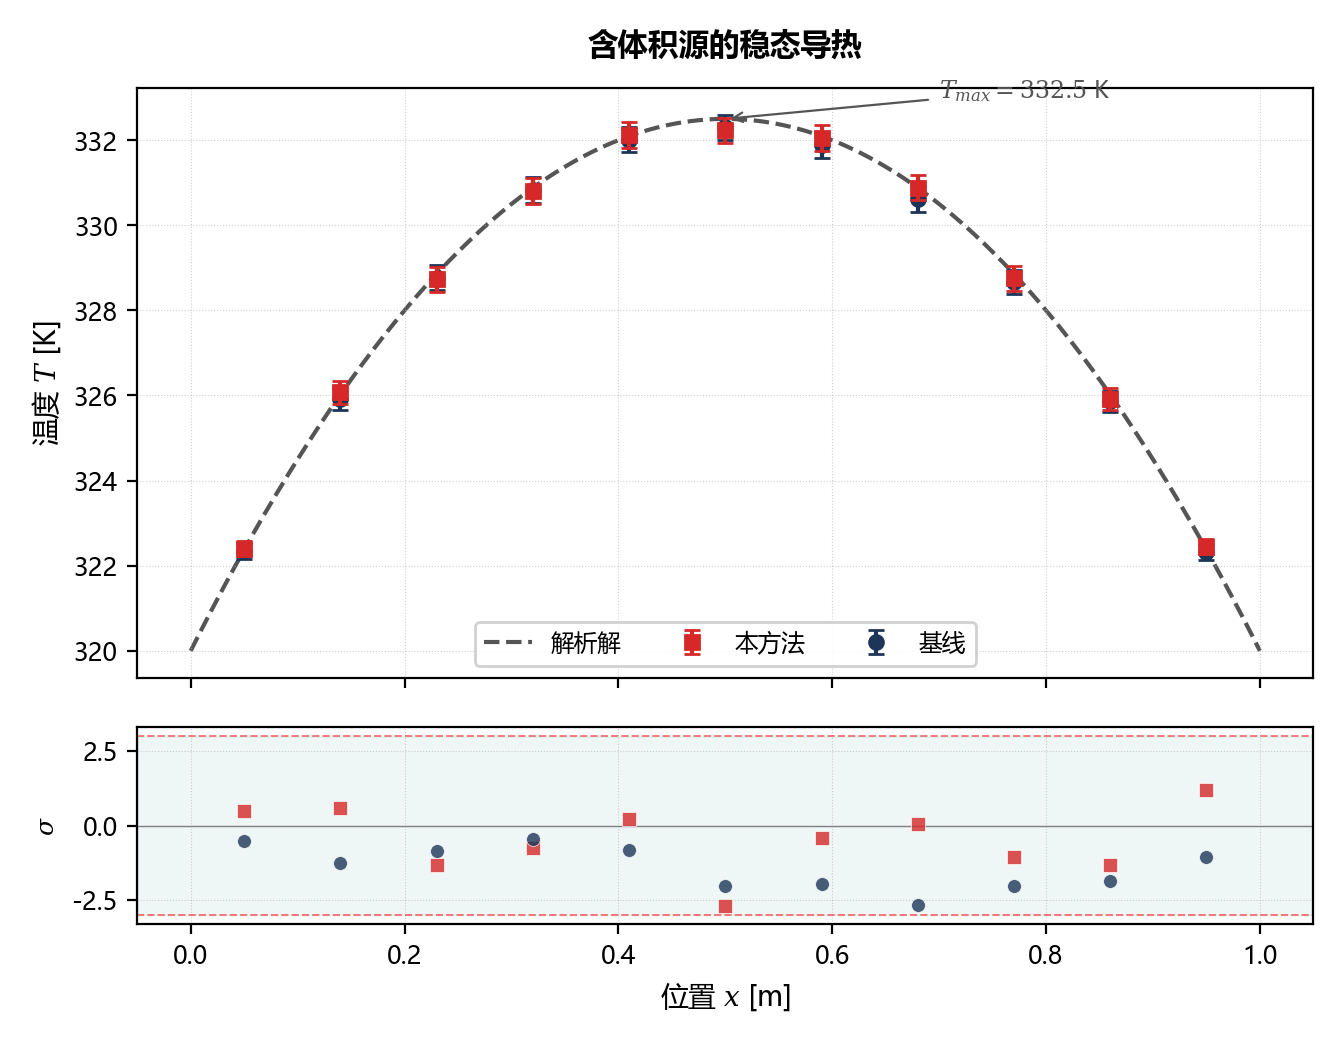
\includegraphics[width=0.85\textwidth]{Figures/Consistency/fig1_a2_parabola.png}
  \bicaption{稳态导热体积热源验证}{Steady-state volumetric heat source verification}
  \label{fig:consistency-a2}

  \small
  Wavefront 求解器（红色方块）与递归求解器（蓝色圆点）均精确复现倒抛物线解析解（灰色虚线），下方面板显示标准化偏差 $\sigma$ 均在 $\pm 3$ 以内。
\end{figure}

\paragraph{实验二：多材料界面——接触热阻折线族}

两种导热系数不同的材料（$\lambda_1 = 0.1$，$\lambda_2 = 0.2$~W/(m$\cdot$K)）拼接于 $x_0 = 3$~m 处，总长 $L = 4$~m，左端 $T_0 = 0$~K，右端 $T_L = 100$~K。界面接触热阻 $R$~[m$^2\cdot$K/W] 引入温度跳跃。稳态热流密度为

\begin{equation}
  \label{eq:a3-heatflux}
  q = \frac{T_L - T_0}{x_0/\lambda_1 + R + (L - x_0)/\lambda_2}
\end{equation}

\noindent 两侧温度分布均为线性：左侧 $T(x) = T_0 + (q/\lambda_1)\,x$，右侧 $T(x) = T_L - (q/\lambda_2)(L-x)$，界面温度跳跃 $\Delta T = q R$。5 个 $R$ 值（0.01, 0.1, 1, 10, 100）形成扇形展开的分段折线族——$R$ 越大，界面跳跃越大，曲线越平缓。GPU 以 5 组 $R$ 值系统扫描（40 个数据点），CPU 以随机 $R$ 采样（16 个数据点）从两个互补角度验证，全部通过 $3\sigma$ 检验（图~\ref{fig:consistency-a3}）。

\begin{figure}[htbp]
  \centering
  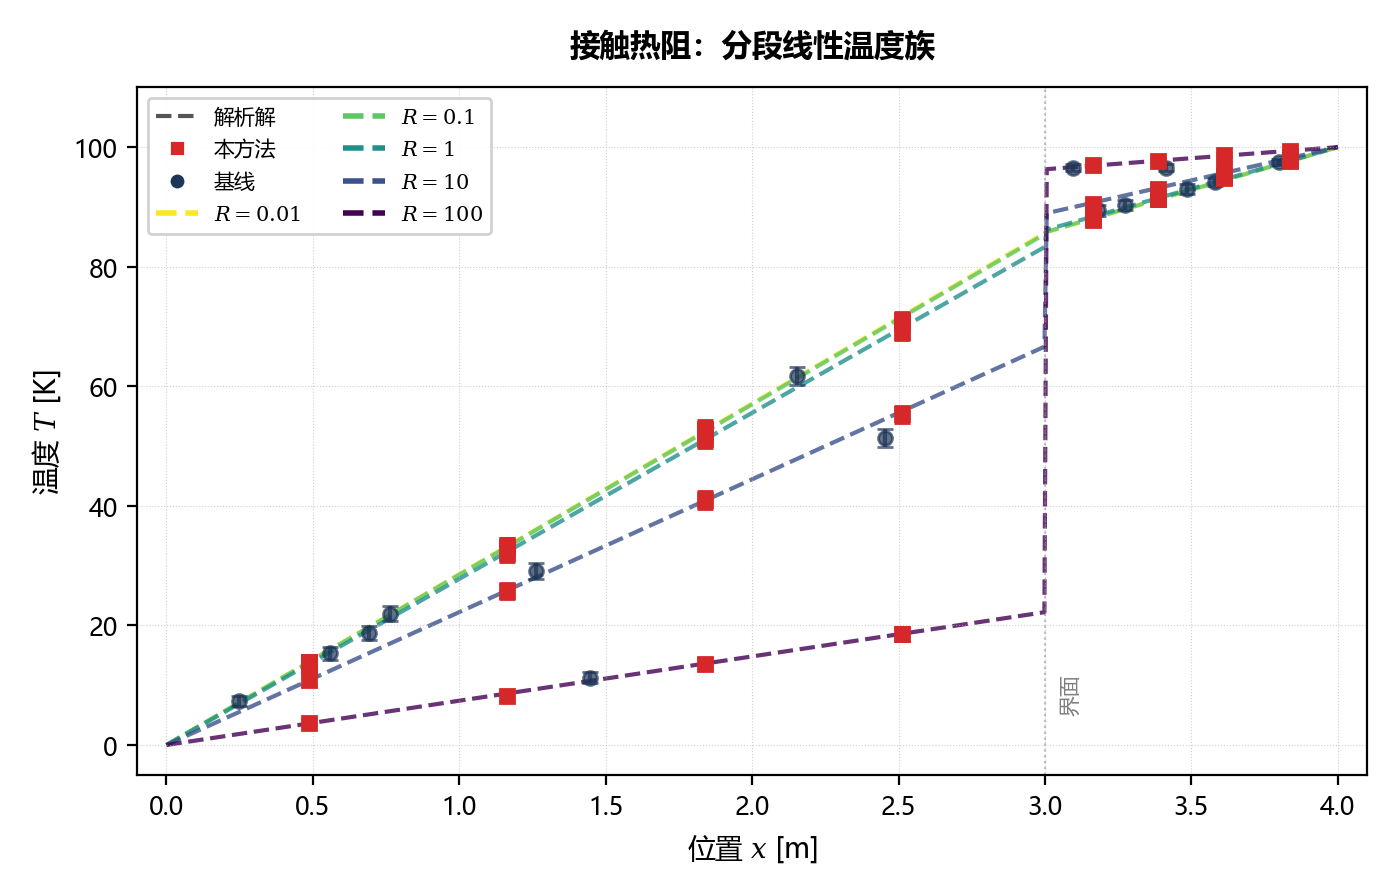
\includegraphics[width=0.85\textwidth]{Figures/Consistency/fig2_a3_contact_resistance.png}
  \bicaption{多材料接触热阻验证}{Multi-material contact resistance verification}
  \label{fig:consistency-a3}

  \small
  5 组 $R$ 值形成扇形折线族，GPU 40 个探针（红色方块）排列于各自对应折线上，CPU 16 个随机探针（蓝色圆点）散布于折线族中，均在 $3\sigma$ 区间内。
\end{figure}

\paragraph{实验三：对流换热瞬态——指数衰减}

立方体固体初始温度 $T_0 = 280$~K，六面暴露于均匀流体温度 $T_\infty = 325$~K，对流换热系数 $H$。集总参数模型（Biot 数 $\ll 1$）给出精确的指数趋近解：

\begin{equation}
  \label{eq:d1-exponential}
  T(t) = T_0\, e^{-\nu t} + T_\infty\left(1 - e^{-\nu t}\right)
\end{equation}

\noindent 其中衰减率 $\nu = 6H/(\rho c_p) = 1.2$~s$^{-1}$（六面均匀对流），时间常数 $\tau = 1/\nu \approx 0.83$~s。这是牛顿冷却定律最直观的时域表现——温度从 280~K 指数升温，渐近趋于 325~K。图~\ref{fig:consistency-d1} 展示了 4 个瞬态时刻和稳态极限处的验证结果，GPU（9/9）与 CPU（5/5）全部通过 $3\sigma$ 检验，精确复现了指数衰减动力学。稳态区间 GPU 5 个不同空间位置探针均给出 $E \approx 325.0$~K，验证了集总参数模型``稳态温度与空间位置无关''的物理预测。

\begin{figure}[htbp]
  \centering
  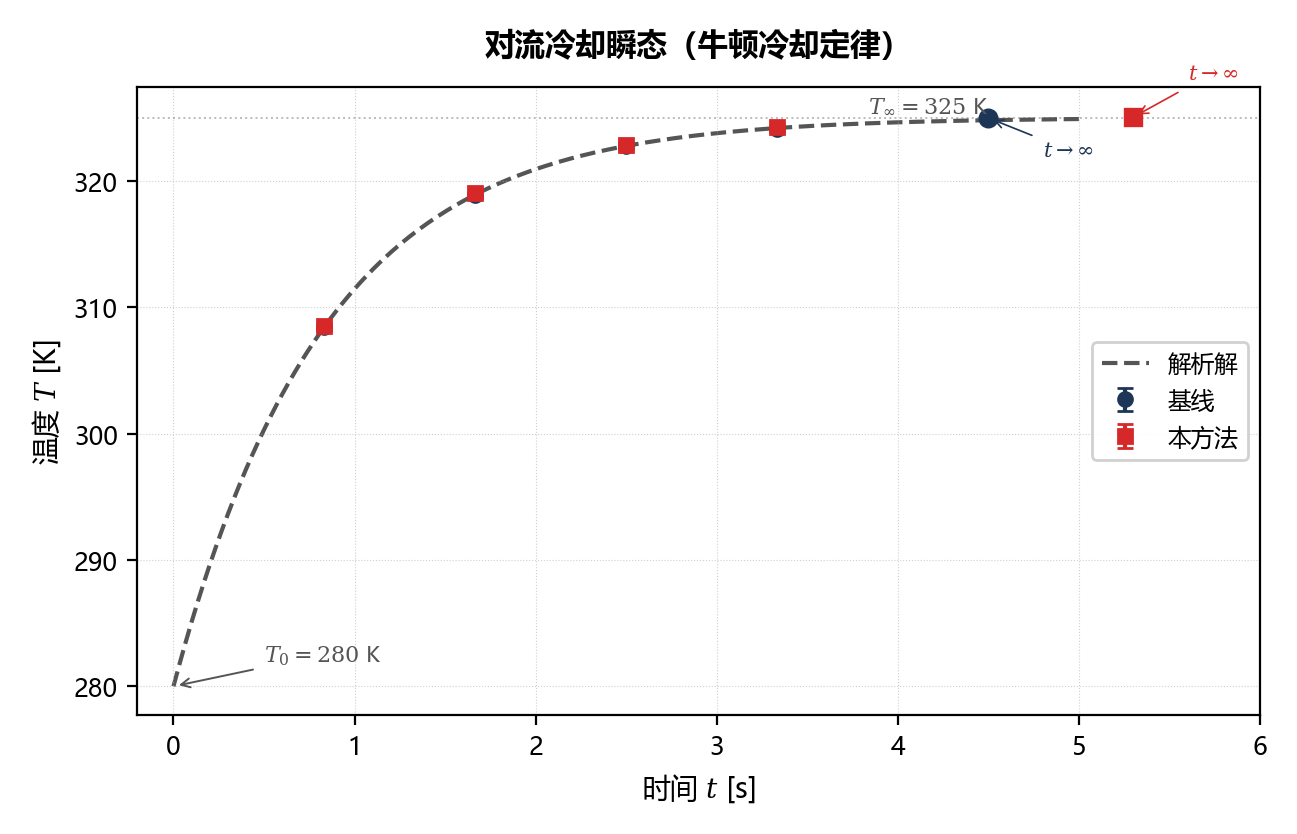
\includegraphics[width=0.85\textwidth]{Figures/Consistency/fig3_d1_convection.png}
  \bicaption{对流换热瞬态验证}{Transient convective heat transfer verification}
  \label{fig:consistency-d1}

  \small
  Wavefront 求解器（红色方块）与递归求解器（蓝色圆点）均精确复现牛顿冷却定律的指数衰减解析解（灰色虚线），渐近趋于流体温度 $T_\infty = 325$~K。
\end{figure}

\paragraph{实验四：扩散方程精确解——$\sin \times \exp$}

采用制造解法（Method of Manufactured Solutions）：在超形体几何体上预设解析温度场作为 Dirichlet 边界条件，由 MC 求解器反算内部温度后与预设解对比。解析解为稳态调和多项式与瞬态正弦本征模的叠加：

\begin{equation}
  \label{eq:e3-sinexp}
  T(x,y,z,t) = \frac{1}{\lambda}\left[B_1(x^3 z - 3xy^2 z) + B_2 \sin\frac{\pi x}{4}\sin\frac{\pi y}{4}\sin\frac{\pi z}{4}\cdot e^{-\alpha k^2 t}\right]
\end{equation}

\noindent 其中 $B_1 = 10$，$B_2 = 1000$，热扩散系数 $\alpha = \lambda/(\rho c_p) = 0.002$~m$^2$/s，$k^2 = 3(\pi/4)^2$，时间常数 $\tau = 1/(\alpha k^2) \approx 270$~s。图~\ref{fig:consistency-sinexp} 以双子图展示验证结果：左图固定空间点 $(0.2, 0.3, 0.4)$ 的温度随时间的指数衰减（对数时间轴，0.5\textasciitilde1000~s），右图固定时刻 $t = 5$~s 的温度沿 $x$ 轴的正弦空间分布。GPU（23/23）与 CPU（24/24）数据点均精确落在解析曲线上，同时验证了空间本征模式和时间积分的正确性。

\begin{figure}[htbp]
  \centering
  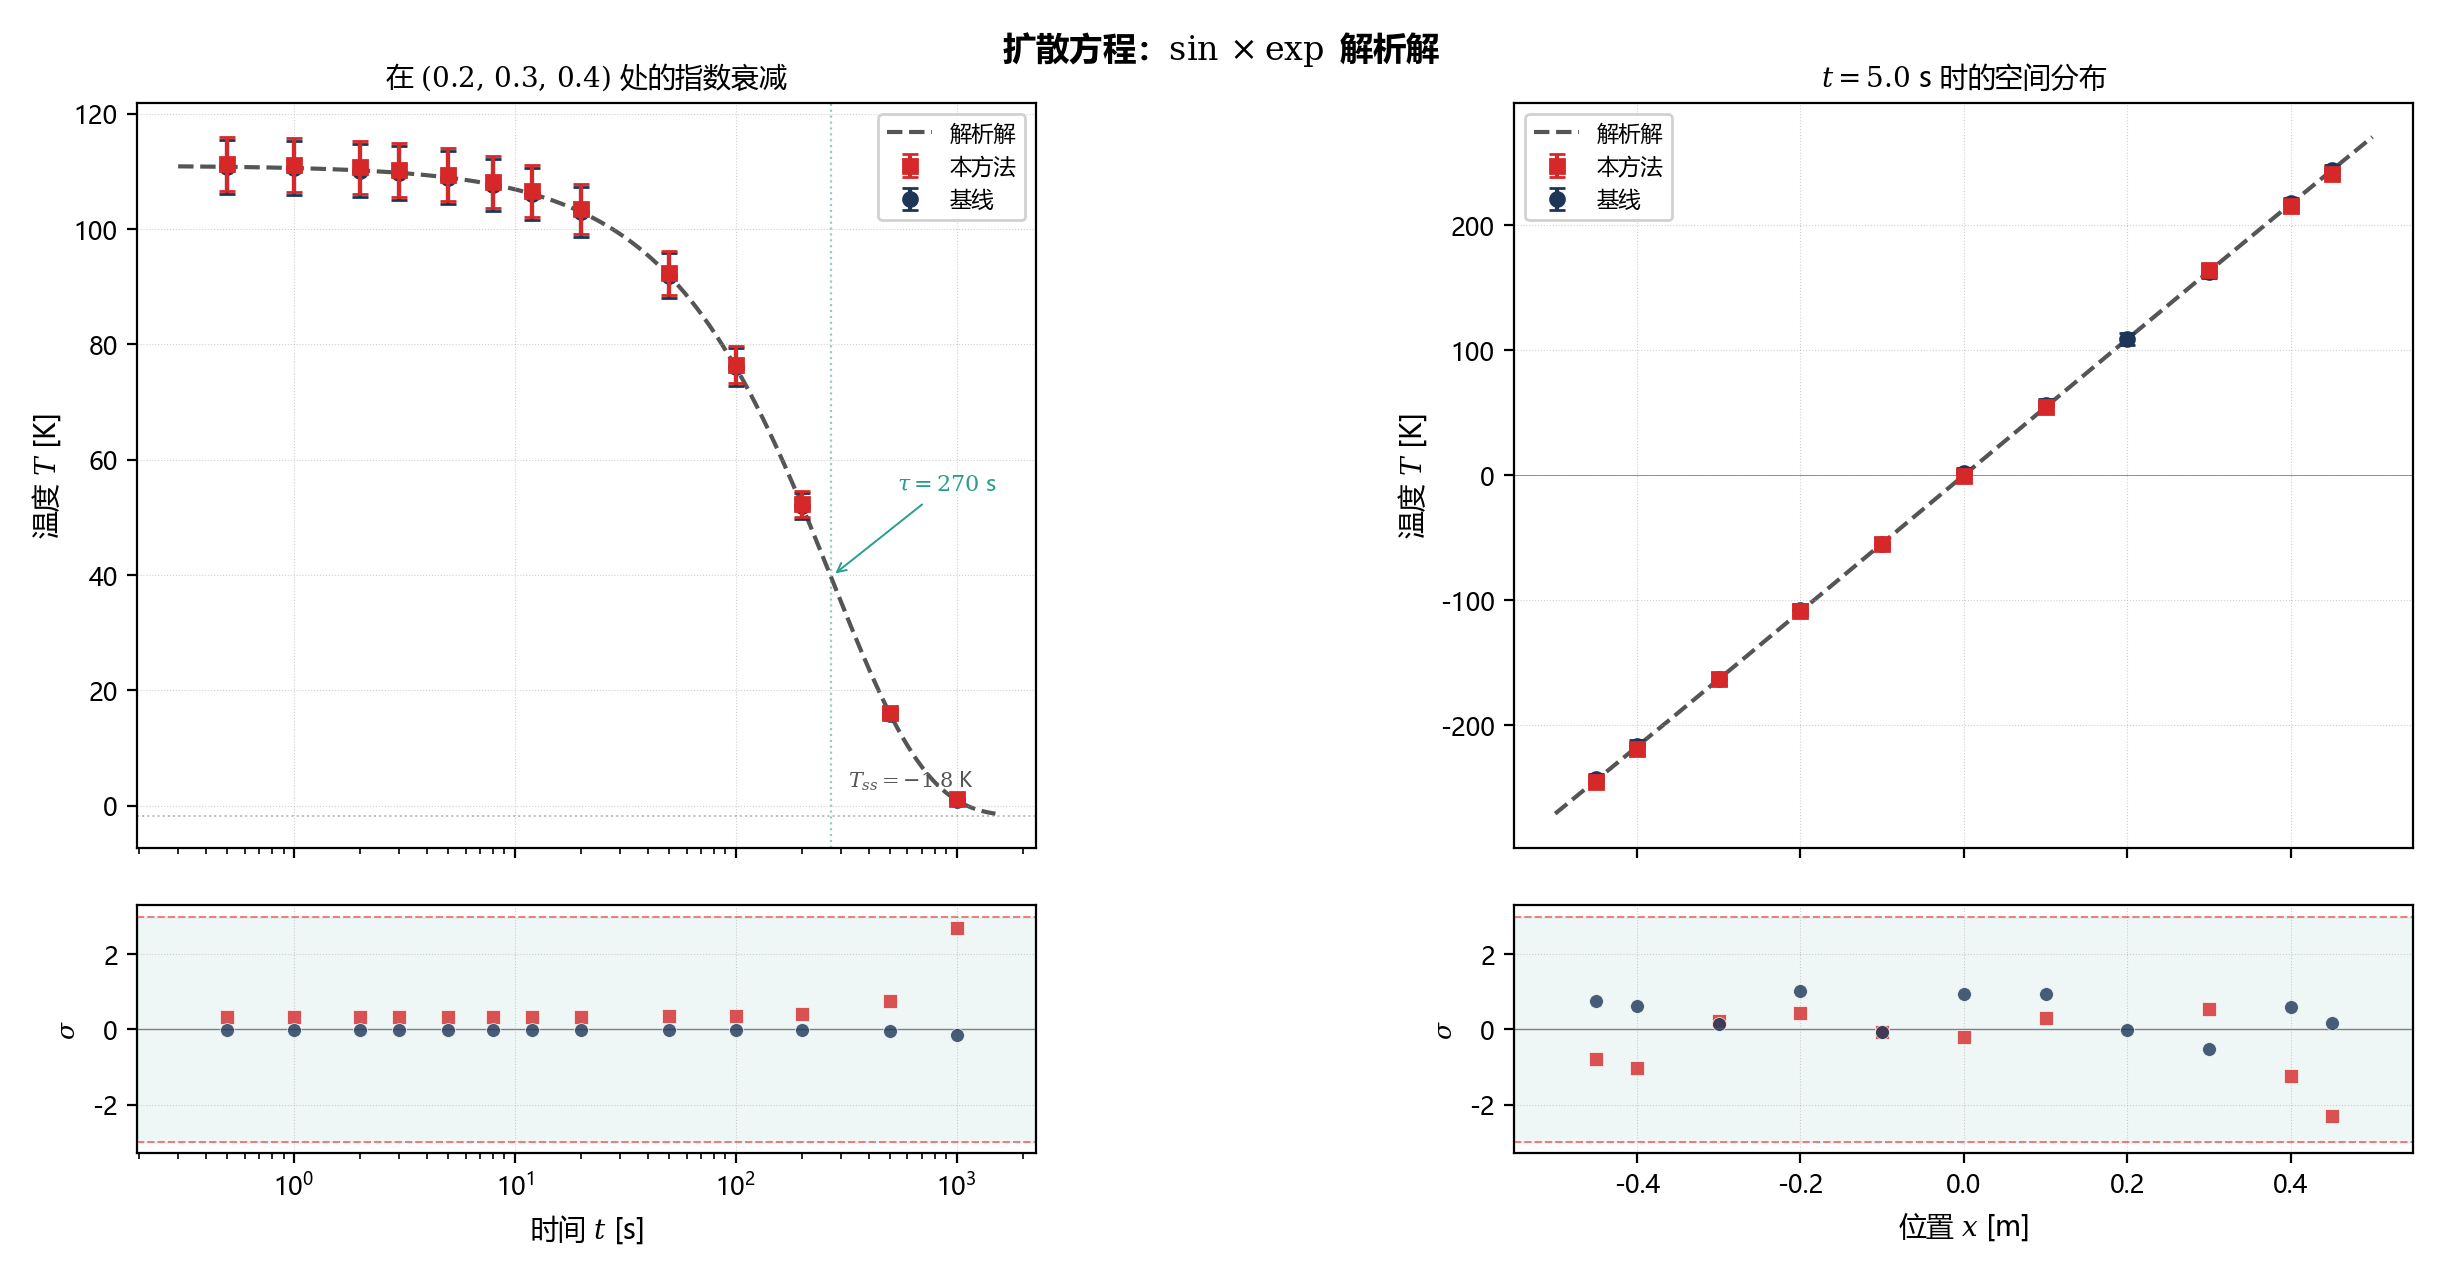
\includegraphics[width=0.9\textwidth]{Figures/Consistency/fig4_e3_sin_exp.png}
  \bicaption{扩散方程 $\sin \times \exp$ 精确解验证}{Diffusion equation $\sin \times \exp$ exact solution verification}
  \label{fig:consistency-sinexp}

  \small
  Wavefront 求解器（红色方块）与递归求解器（蓝色圆点）均精确复现时域指数衰减（左）与空间正弦分布（右）的解析解（灰色虚线），下方面板显示标准化偏差 $\sigma$ 均不超过 3。
\end{figure}

\paragraph{实验五：多域耦合瞬态——流体-固体-大气}

流体域、固体域与大气层组成的多介质耦合系统，从均匀初温 300~K 开始瞬态热响应。辐射边界条件驱动能量输入，参考值来自高精度数值求解。双探针设计揭示双时间尺度特征：流体探针 $(1.5, 1.5, 1.5)$ 接近辐射边界，约 3000~s 达稳态（$\sim$310~K）；固体探针 $(3.04, \cdot, \cdot)$ 热惯性大，超过 10000~s 仍在缓慢爬升（$\sim$305~K）。图~\ref{fig:consistency-e5} 展示了 0\textasciitilde10000~s 范围内两条趋近曲线，GPU（19/19）与 CPU（40/40）均精确跟踪参考曲线。该测试同时涵盖多域耦合、辐射边界条件、长时间瞬态和双时间尺度四个验证维度，是最接近工业真实场景的验证。

\begin{figure}[htbp]
  \centering
  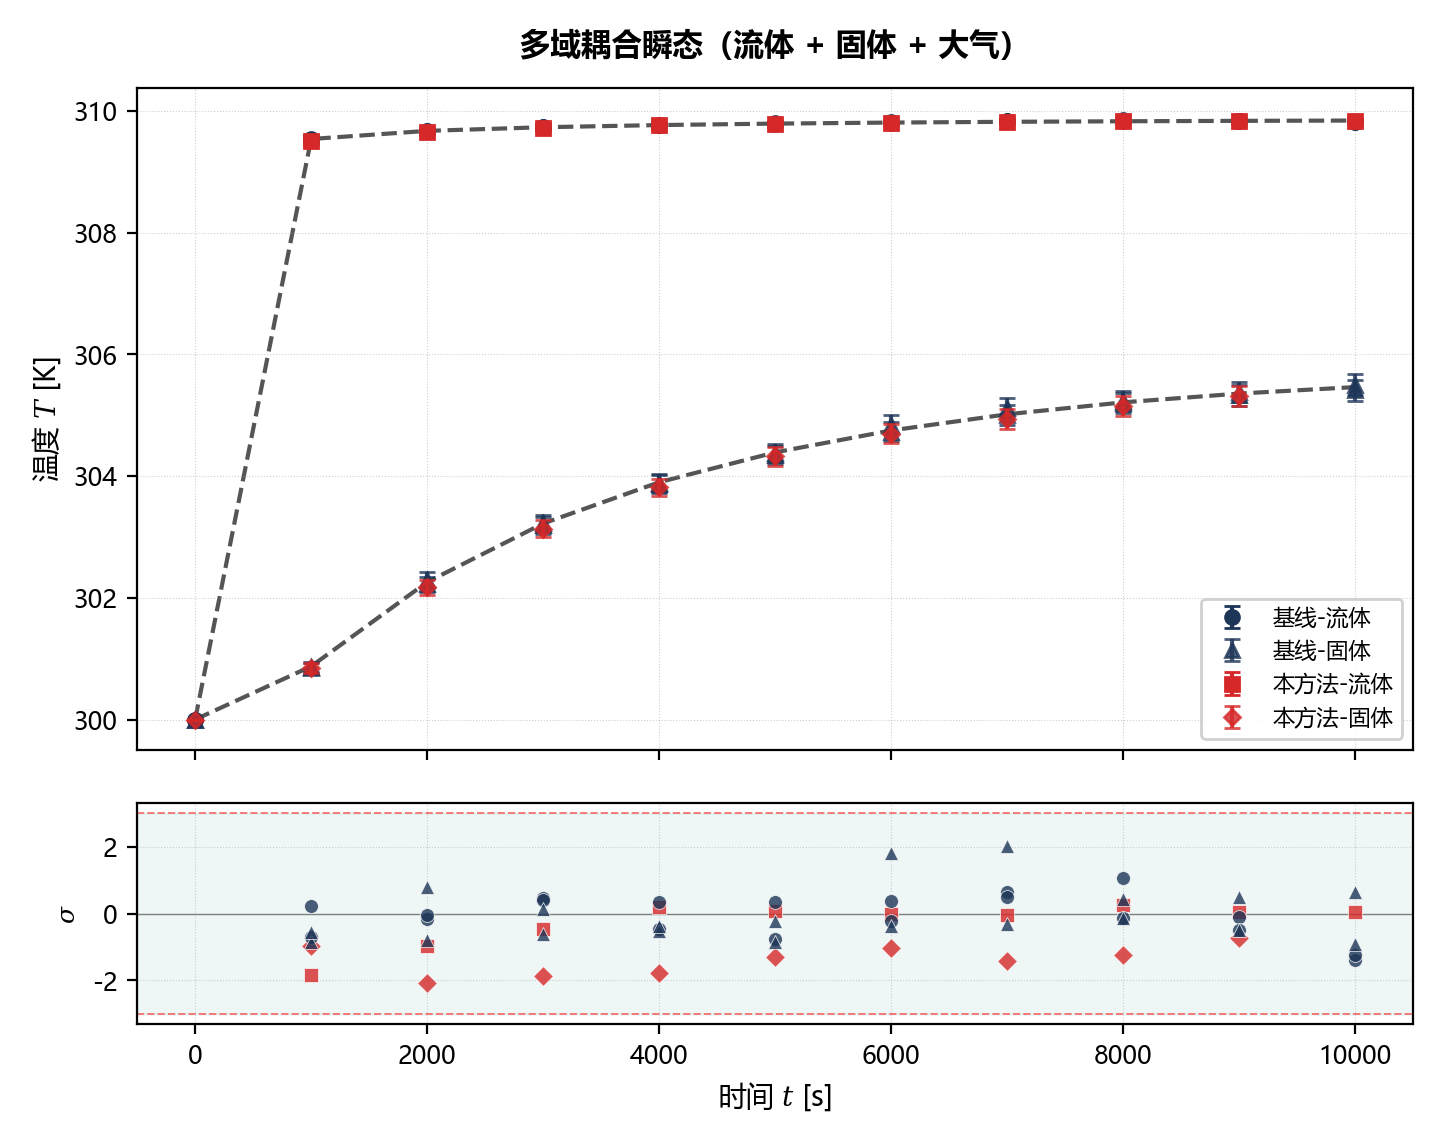
\includegraphics[width=0.85\textwidth]{Figures/Consistency/fig5_e5_multidomain.png}
  \bicaption{多域耦合瞬态验证}{Multi-domain transient verification}
  \label{fig:consistency-e5}

  \small
  流体探针（快响应，$\sim$3000~s 达稳态）与固体探针（慢响应，$>$10000~s）的温度演化均被两种架构精确复现，下方面板显示 $\sigma$ 均在 $\pm 3$ 以内。
\end{figure}

\paragraph{统计汇总}

表~\ref{tab:consistency-suite} 列出的 13 个场景按物理复杂度构成四级递进阶梯：第一级为单模态稳态（纯传导），覆盖体源、多材料异质性与介质嵌套，验证传导求解与材料处理的正确性；第二级为多模态稳态，引入辐射—传导耦合、Picard 多阶迭代与外部环境（太阳直射、天空漫射）边界，验证界面耦合与外部辐射条件的正确性；第三级引入时间维度，覆盖对流指数衰减、空间非均匀对流系数与扩散方程时空精确解，验证时间积分与瞬态边界的正确性；第四级为多域耦合瞬态全耦合场景，验证多介质域之间的完整耦合。前述 5 个详述实验已从各级中各选至少一个代表，优先采用具有封闭解析解的场景以提供最严格的基准对照；其余 8 个辅助测试在同级内覆盖正交参数变体，保证验证的系统性。全部 282 个有效数据点（GPU 134 + CPU 148）均通过 $3\sigma$ 检验。

GPU 和 CPU 的 $\sigma$ 均值分别为 0.816 和 0.739，最大标准化偏差分别为 2.708 和 2.676，均远低于 $3\sigma$ 阈值。图~\ref{fig:consistency-summary} 汇总全部 13 个测试的统计结果：左图 $\sigma$ 分布直方图显示两种架构分布形态高度一致，峰值集中于 $0$\textasciitilde$1\sigma$ 区间；右图 Parity 散点图中全量数据点紧密分布于 $E = T_{\mathrm{ref}}$ 对角线上，温度覆盖 $-244$~K 至 $2068$~K。

\begin{figure}[htbp]
  \centering
  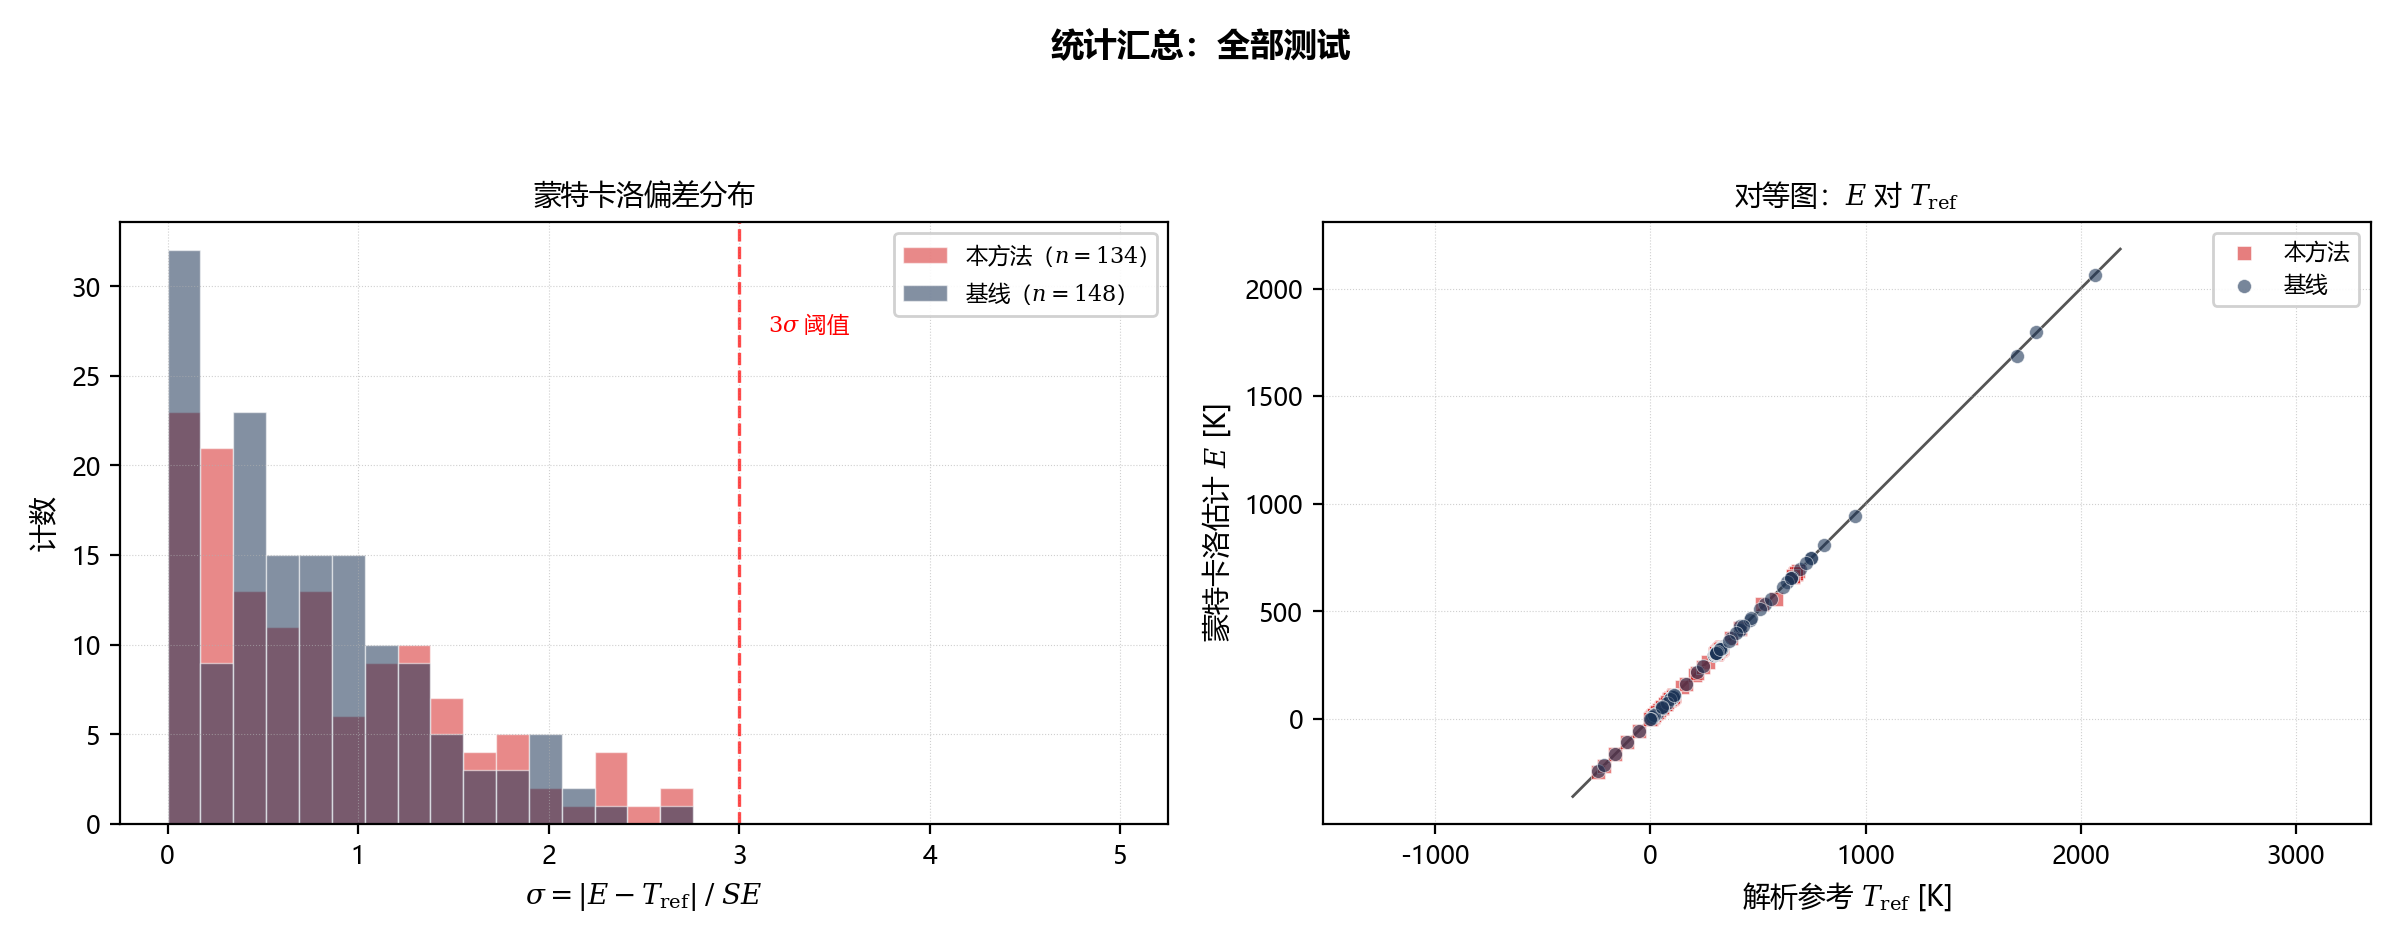
\includegraphics[width=0.9\textwidth]{Figures/Consistency/fig6_summary.png}
  \bicaption{全测试体系统计汇总}{Statistical summary of all tests}
  \label{fig:consistency-summary}

  \small
  (a) $\sigma$ 分布直方图——GPU 134 个与 CPU 148 个数据点均在 $3\sigma$ 阈值（红色虚线）以内；(b) 估计值 vs 参考值 Parity 散点图——全量数据点紧密分布于 $E = T_{\mathrm{ref}}$ 对角线。
\end{figure}

在共享探针位置的测试中，GPU 与 CPU 的标准误差（SE）比率为 $1.00 \pm 0.05$，确认两种架构的蒙特卡洛估计器方差结构等价——Wavefront 批处理与递归求解器逐路径两种调度策略不影响统计收敛行为。

\subsubsection{端到端统计等价性检验}

\paragraph{指标选择}

图像质量评估领域常用 PSNR（峰值信噪比）和 SSIM（结构相似性）作为衡量指标，它们以像素差的 $\ell_2$ 范数或局部结构相关性来量化两幅图像的``距离''。然而，这两类指标均不适用于蒙特卡洛求解器的等价性验证。原因在于：PSNR 和 SSIM 隐含一个确定性参考图（ground truth），将差异解读为确定性``失真''；而两个蒙特卡洛估计器对同一场景的输出本身就是随机变量——每个像素不仅有期望值，还有由采样量决定的标准误差。两幅蒙特卡洛图像之间的逐像素差异是两组随机变量之差，应使用假设检验框架判定其差异是否超出随机噪声的统计预期，而非用距离度量来衡量。此外，PSNR 依赖于信号动态范围，对于温度场（绝对温标，无界）缺乏自然的参考量程；SSIM 的局部窗口加权会平滑高频结构性偏差。

因此，本节采用逐像素双样本 $Z$ 检验：对 Wavefront 求解器和递归求解器输出的每个像素独立构造检验统计量，利用蒙特卡洛估计器自身提供的标准误差进行归一化，直接判定差异是否可由随机抽样噪声解释。

\paragraph{检验方法}

在 porous 场景（$512 \times 512$，128 SPP）上，对 Wavefront 求解器和递归求解器的逐像素估计量进行双样本 $Z$ 检验：

\begin{equation}
  \label{eq:z-test}
  Z_{x,y} = \frac{|E_{\mathrm{gpu}} - E_{\mathrm{cpu}}|}{\sqrt{\mathrm{SE}_{\mathrm{gpu}}^2 + \mathrm{SE}_{\mathrm{cpu}}^2}}
\end{equation}

\noindent 其中 $E$ 为像素温度估计值，$\mathrm{SE}$ 为蒙特卡洛标准误差。若两种架构的估计器无偏且等价，$Z_{x,y}$ 应服从标准半正态分布（$|Z|$ 分布），在显著性水平 $\alpha = 0.05$ 下期望仅约 5\% 的像素因随机噪声被``误拒''。共 262{,}144 个像素中有 153{,}976 个有效像素（排除背景和零方差像素）。

\paragraph{多重比较校正}

逐像素检验涉及 $N = 153{,}976$ 次独立假设检验，属于典型的大规模多重比较问题。若不加校正，在 $\alpha = 0.05$ 下纯随机噪声即可产生约 $0.05 \times 153{,}976 \approx 7{,}699$ 个``假阳性''像素，使得单像素显著性失去判断能力。为此采用两种互补的多重比较校正方法：

\textbf{Bonferroni 校正}是最保守的全族错误率（FWER）控制方法：将每个像素的显著性阈值收紧为 $\alpha/N$，即 $\alpha_{\mathrm{Bonf}} = 0.05/153{,}976 \approx 3.25 \times 10^{-7}$，对应的 $Z$ 阈值约为 5.05。它控制的是``至少一个假阳性''的概率不超过 $\alpha$——只要有任一像素的 $Z$ 值超过 5.05，就有充分理由怀疑系统性偏差存在。Bonferroni 校正虽然以牺牲统计功效为代价换取极强的保守性，但这恰恰符合本文的验证需求：我们不关心``多少像素有差异''，而关心``是否存在任何真实差异''。

\textbf{Benjamini-Hochberg (BH) 假发现率（FDR）校正}控制的是在拒绝集合中假阳性所占比例的期望值不超过 $q$（本文取 $q = 0.05$）。其步骤为：将 $N$ 个 $p$ 值从小到大排序为 $p_{(1)} \leq \cdots \leq p_{(N)}$，找到满足 $p_{(k)} \leq k \cdot q / N$ 的最大 $k$，拒绝前 $k$ 个假设。BH-FDR 比 Bonferroni 宽松，统计功效更高，若它也报告零显著像素，则进一步排除了 Bonferroni 过于保守而遗漏弱信号的可能性。两种校正方法从严-宽两个极端形成包夹：Bonferroni 保证无假阳性，BH-FDR 保证不遗漏成片的弱偏差。

\paragraph{检验结果}

表~\ref{tab:pixel-consistency} 汇总了检验结果。

\begin{table}[htbp]
  \centering
  \bicaption{porous 场景逐像素统计等价性检验结果}{Per-pixel statistical equivalence test results on the porous scene}
  \label{tab:pixel-consistency}
  \small
  \begin{tabular}{lcc}
    \toprule
    指标 & 结果 & 纯 MC 噪声期望值 \\
    \midrule
    有效像素数                          & 153{,}976               & — \\
    Mean $Z$                            & 0.8057                  & $\sim$0.7979（半正态均值）\\
    原始拒绝率 ($\alpha = 0.05$)        & 5.10\%                  & $\sim$5\% \\
    Bonferroni 校正后显著像素           & \textbf{0}              & $\sim$0 \\
    Benjamini-Hochberg FDR 校正后显著像素 & \textbf{0}            & $\leq$5\% \\
    \bottomrule
  \end{tabular}
\end{table}

Mean $Z = 0.8057$ 与理论半正态均值 $\sqrt{2/\pi} \approx 0.7979$ 的偏差仅为 1.0\%，表明 $Z$ 值分布与零假设预测精确吻合。原始拒绝率 5.10\% 与 $\alpha = 0.05$ 的预期一致，无超额拒绝。经 Bonferroni 校正（$Z$ 阈值 $\approx 5.05$）后零显著像素，说明不存在任何单像素级别的系统性偏差；经 BH-FDR 校正后同样零显著像素，排除了成片弱偏差被 Bonferroni 遗漏的可能。判定结果为PASS (strong)：两架构的逐像素差异完全落入蒙特卡洛随机噪声范围。

图~\ref{fig:pixel-consistency} 展示 porous 场景的逐像素诊断结果：$Z$ 值直方图（左）与半正态 Q-Q 图（右）。直方图中观测 $Z$ 分布（蓝色柱）与理论半正态分布（黑色虚线）高度吻合，$z = 1.96$（$\alpha = 0.05$ 阈值）和 Bonferroni 校正阈值以虚线标注，无任何数据点超过后者；Q-Q 图中绝大多数数据点沿对角线紧密排列，尾部无系统性偏离，确认无结构性偏差。

\begin{figure}[htbp]
  \centering
  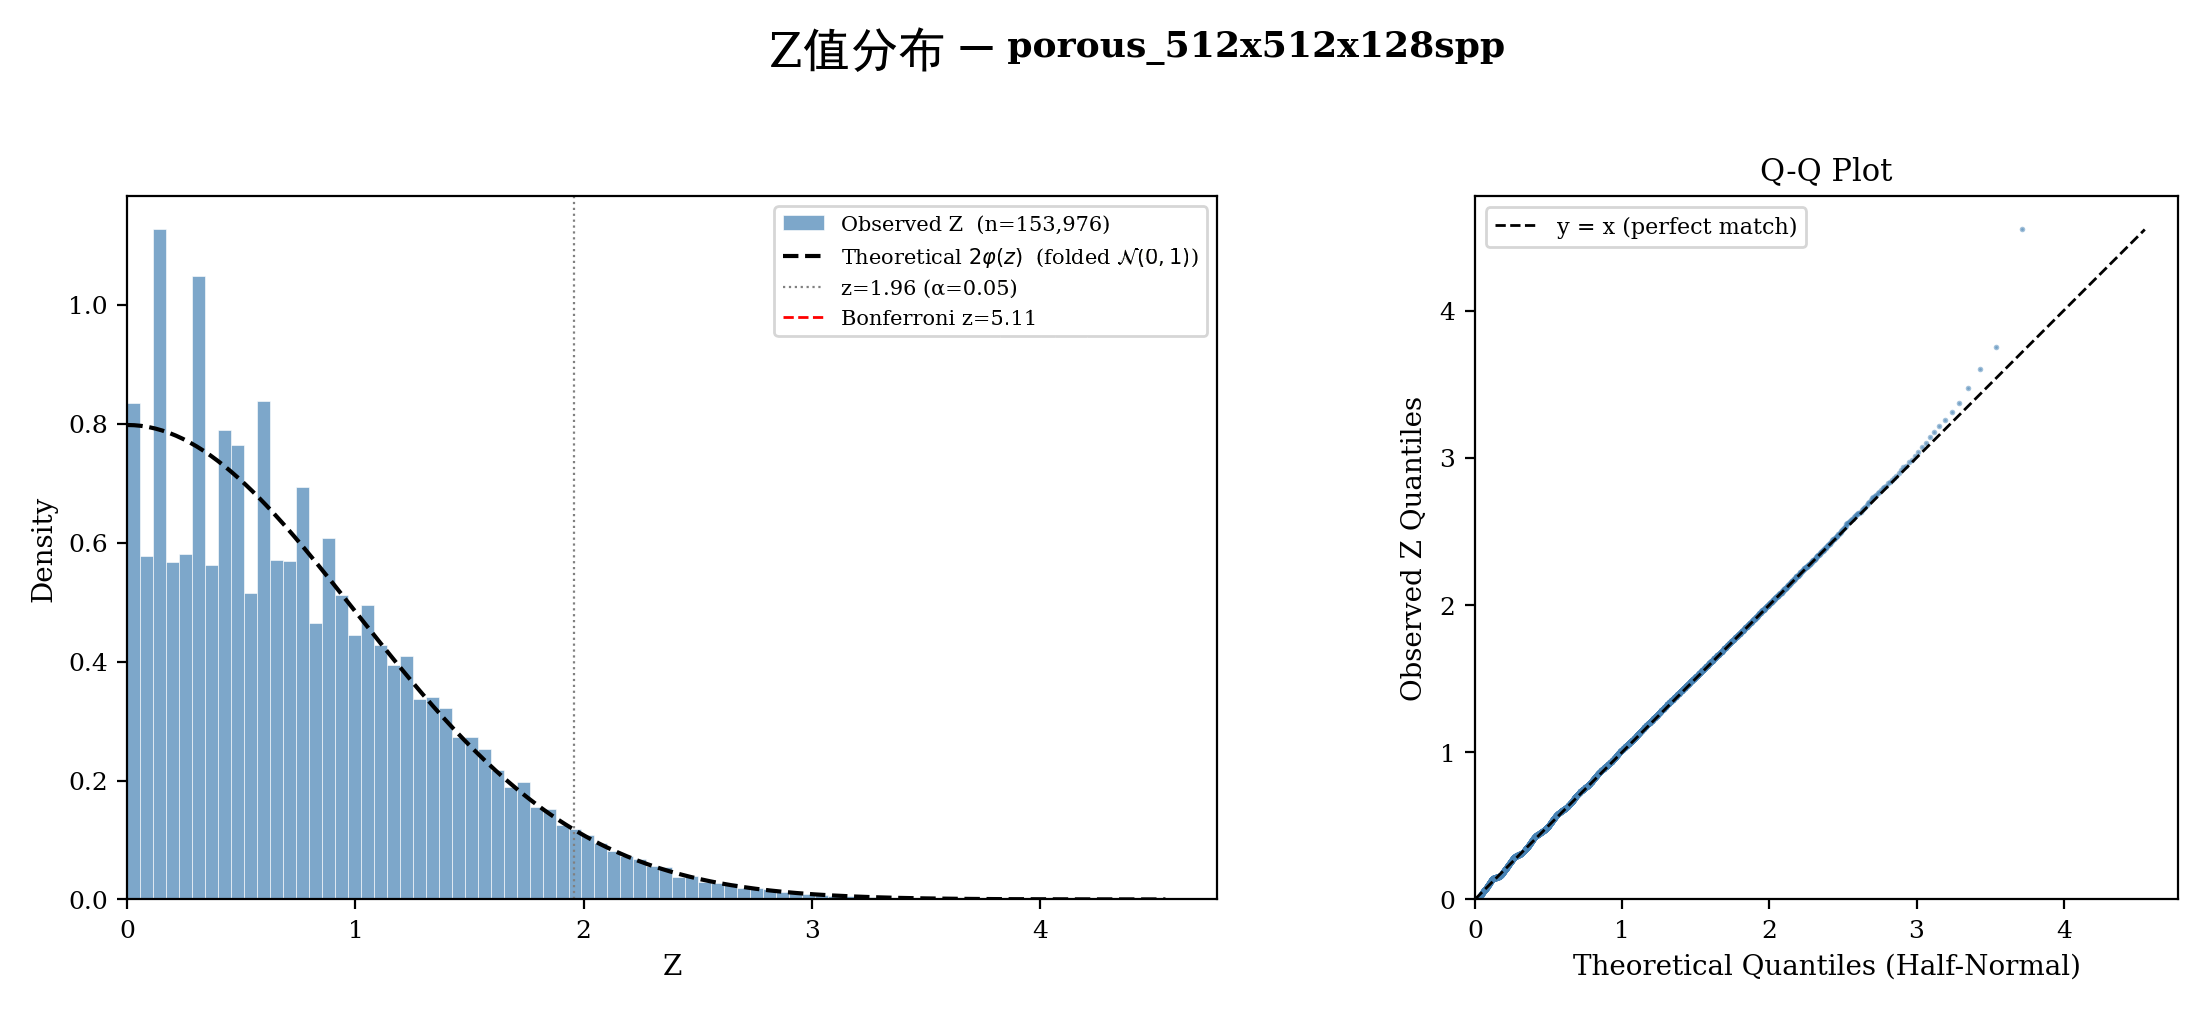
\includegraphics[width=0.85\textwidth]{Figures/Consistency/porous_512x512x128spp_z_diagnostic.png}
  \bicaption{porous 场景逐像素 $Z$ 值诊断（$512 \times 512$，128 SPP）}{Per-pixel $Z$ diagnostic for the porous scene ($512 \times 512$, 128 SPP)}
  \label{fig:pixel-consistency}

  \small
  左图：$Z$ 分布直方图，与半正态理论分布高度吻合，$z = 1.96$（$\alpha = 0.05$）和 Bonferroni 校正阈值以虚线标注；右图：半正态 Q-Q 图，数据点沿对角线紧密排列。
\end{figure}

图~\ref{fig:difference-map} 以空间视图呈现上述统计检验的直观对应：上排分别为 Wavefront 求解器和递归求解器的渲染温度场，视觉上难以分辨差异；下排左图为逐像素绝对温差 $|E_{\mathrm{gpu}} - E_{\mathrm{cpu}}|$，下排右图为逐像素 $Z$ 值空间分布。温差图呈现均匀的低幅噪声纹理，$Z$ 值图中无任何空间聚集的高值区域——这排除了局部几何死角或特定物理模块引入结构性偏差的可能。若 Wavefront 架构在某一物理模块（如 BND 界面耦合或 ENC 包壳查询）存在实现缺陷，对应几何区域的 $Z$ 值将系统性偏高并形成空间聚集，而图中完全不存在这种模式。

\begin{figure}[htbp]
  \centering
  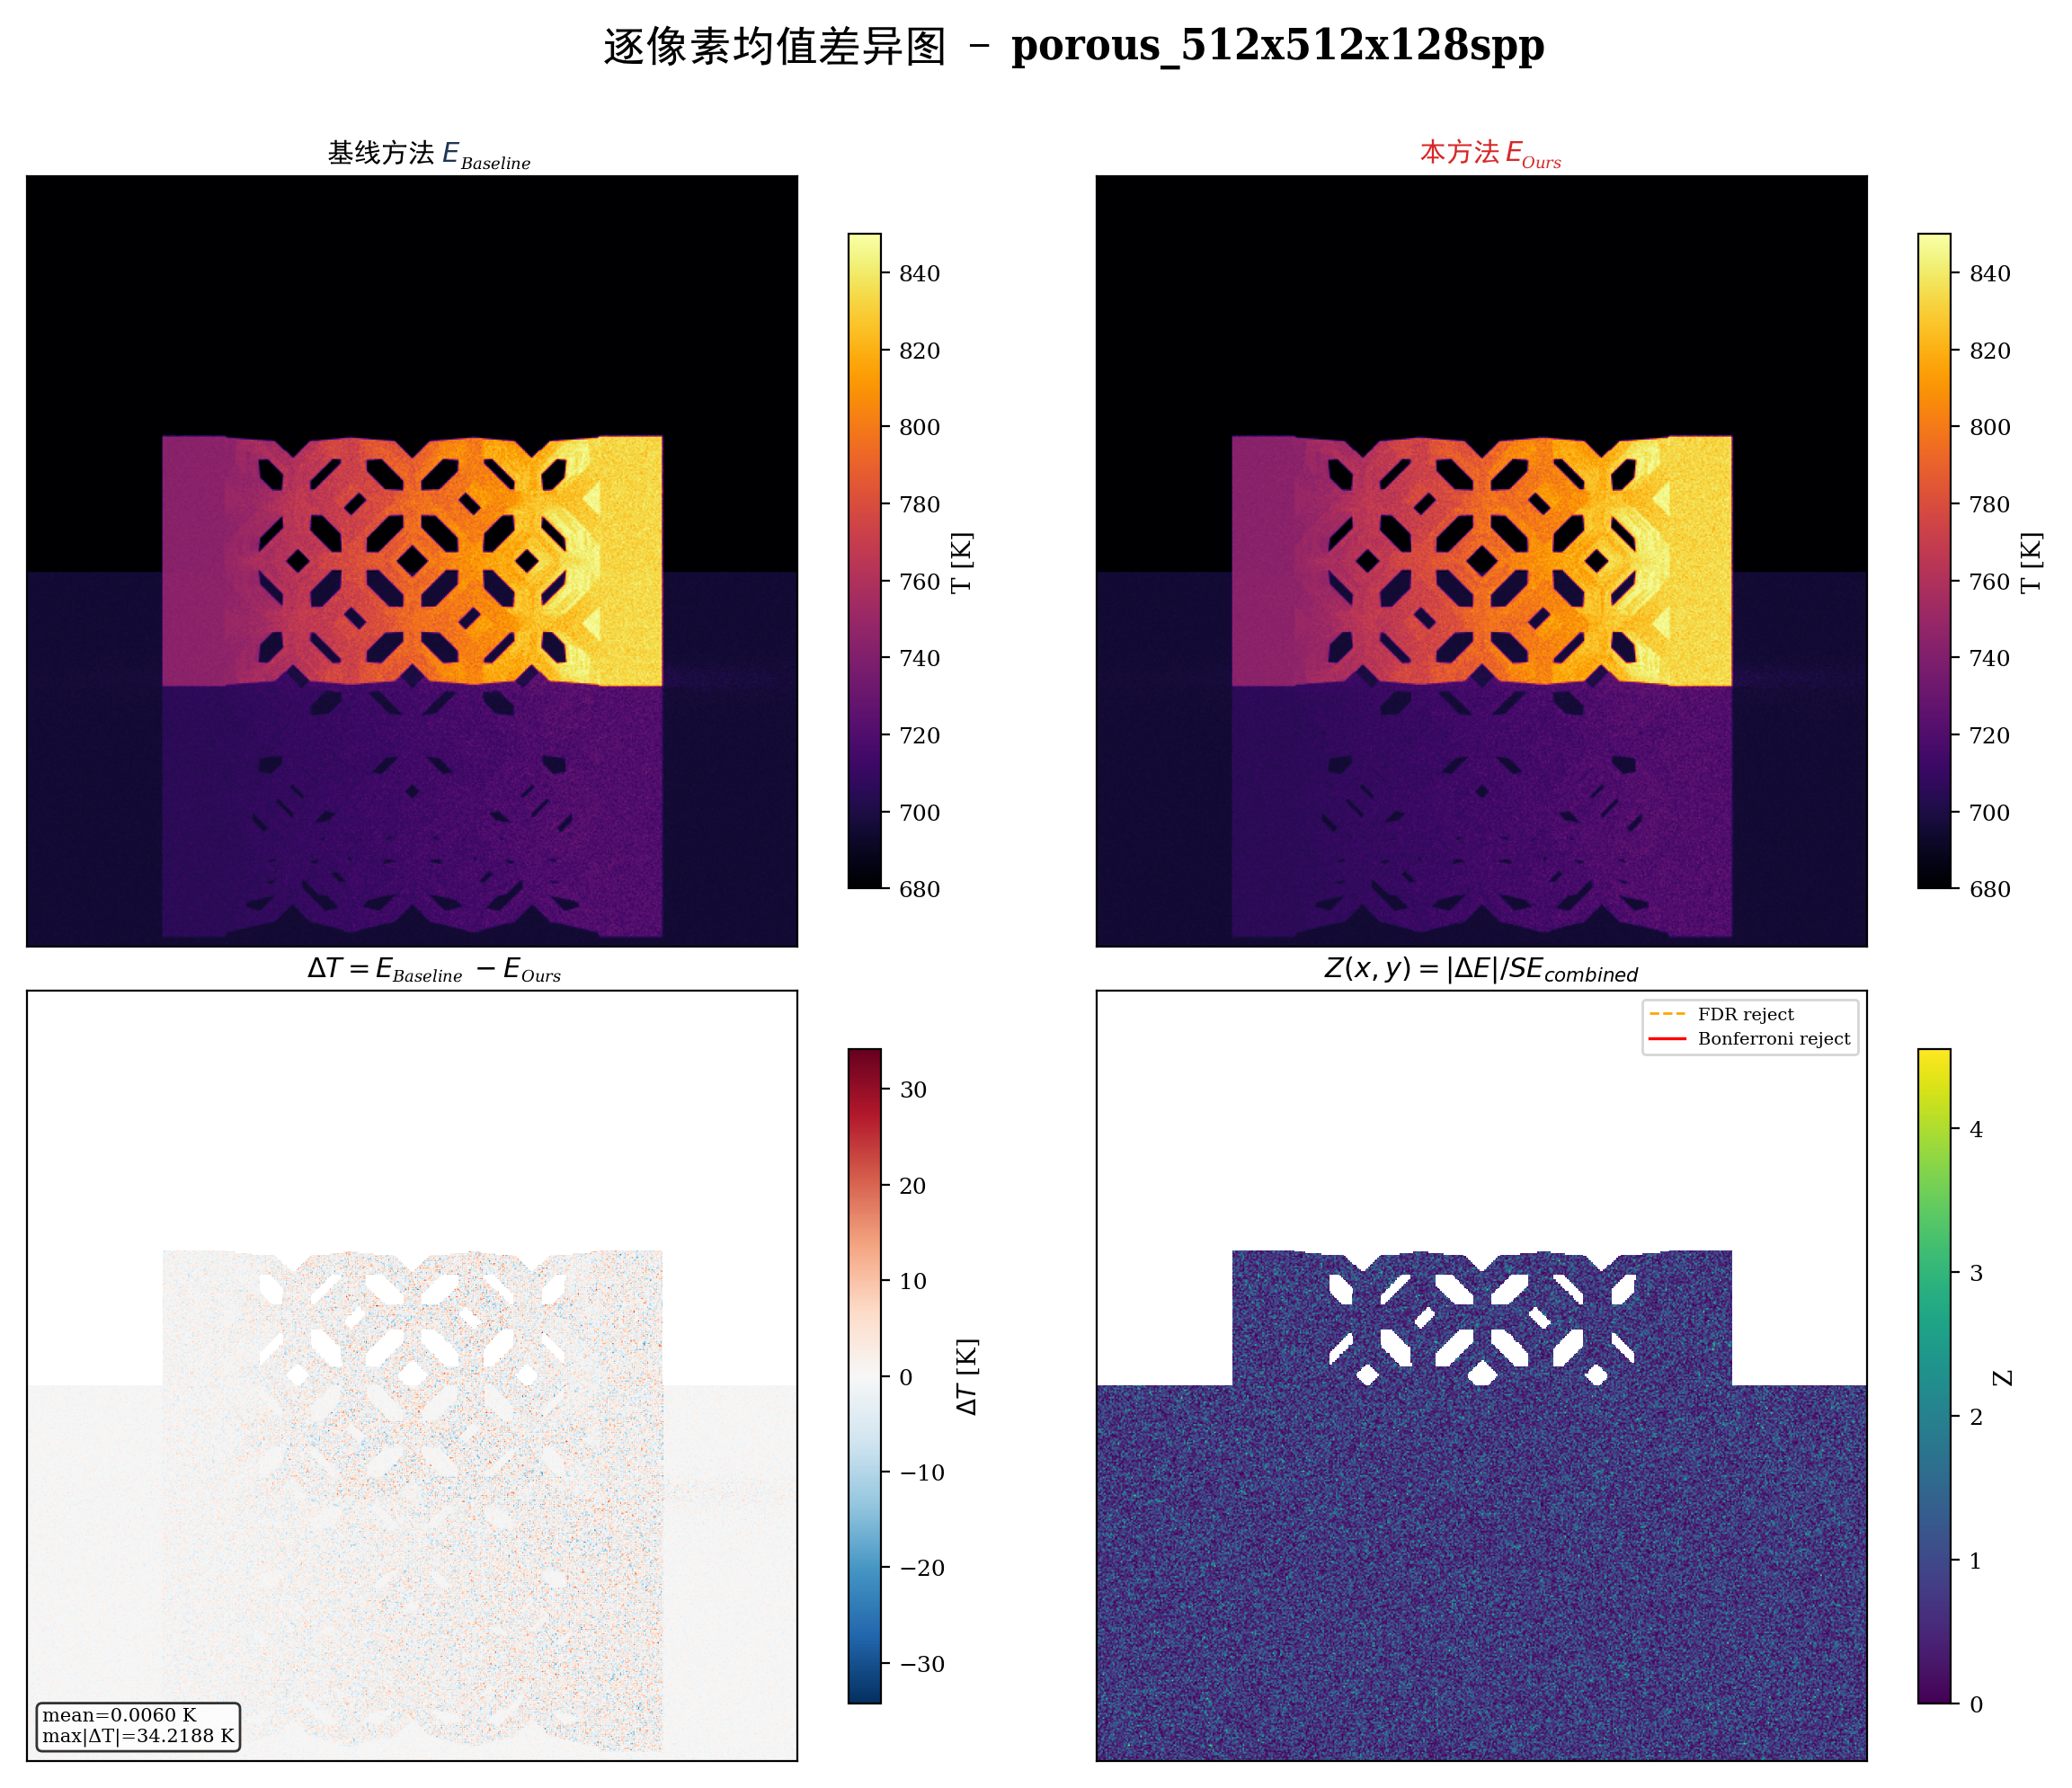
\includegraphics[width=0.9\textwidth]{Figures/Consistency/porous_512x512x128spp_difference_map.png}
  \bicaption{porous 场景逐像素对比（$512 \times 512$，128 SPP）}{Per-pixel comparison of the porous scene ($512 \times 512$, 128 SPP)}
  \label{fig:difference-map}

  \small
  上排：Wavefront 求解器（左）与递归求解器（右）渲染温度场，视觉不可分辨；下排：逐像素绝对温差（左）与 $Z$ 值空间分布（右），差异呈均匀随机噪声，无空间聚集结构。
\end{figure}

综合两个维度的验证结果：物理过程验证证明 Wavefront 实现无系统性物理偏差（13 场景，282 数据点，100\% 通过 $3\sigma$）；端到端统计检验证明两架构在真实耦合场景中的逐像素结果统计等价（153{,}976 有效像素，多重比较校正后零显著差异）。Wavefront 架构改造不引入物理偏差。

\subsection{性能分析}

\subsubsection{端到端性能对比}

表~\ref{tab:performance-comparison} 给出 porous 场景（$320 \times 320$，32 SPP）在不同 CPU 线程数和路径池容量下的端到端墙钟时间和加速比。

\begin{table}[htbp]
  \centering
  \bicaption{porous 场景端到端性能对比}{End-to-end performance comparison on the porous scene}
  \label{tab:performance-comparison}
  \small
  \begin{tabular}{llccc}
    \toprule
    方案 & Pool Size & 线程数 & 墙钟时间 (s) & 加速比 $S$ \\
    \midrule
    Baseline (递归求解器+Embree)  & —      & 32 & 106 & 1.00$\times$ \\
    Baseline (递归求解器+Embree)  & —      & 16 & 155 & 1.00$\times$ \\
    Baseline (递归求解器+Embree)  & —      & 8  & 215 & 1.00$\times$ \\
    \midrule
    Ours (WF+OptiX)        & 8{,}192  & 32 & 104 & 1.02$\times$ \\
    Ours (WF+OptiX)        & 8{,}192  & 16 & 116 & 1.34$\times$ \\
    Ours (WF+OptiX)        & 8{,}192  & 8  & 157 & 1.37$\times$ \\
    \midrule
    Ours (WF+OptiX)        & 16{,}384 & 32 & 234 & 0.45$\times$ \\
    \midrule
    WF+Embree（消融）       & 8{,}192  & 32 & 426 & 0.25$\times$ \\
    \bottomrule
  \end{tabular}
\end{table}

数据呈现三个层次的现象：

（1）在 8\textasciitilde 16 线程的典型工作站配置下，Ours 取得显著加速：8 线程为 $1.37\times$，16 线程为 $1.34\times$。Baseline 的并行度直接受限于 CPU 核心数，其性能随线程数近似线性退化（$155/106 \approx 1.46\times$、$215/106 \approx 2.03\times$）；Ours 的 GPU 查询吞吐不受 CPU 线程数约束，GPU 卸载收益在中等线程配置下最为突出。

（2）当 CPU 线程数达到 32（i9-13900K 全部核心）时，加速比为 $1.02\times$，两种架构达到性能均势（parity）。Baseline 已充分利用全部核心与 Embree 高度优化的 SIMD 光追，CPU 侧状态管理开销抵消了 GPU 查询吞吐增益。

（3）路径池容量从 8{,}192 增至 16{,}384 后，32 线程下墙钟时间从 104~s 跃升至 234~s（$2.25\times$ 退化），退化幅度远超池容量翻倍本身。这是工作集突破缓存容量阈值后的典型 Cache Cliff 行为，直接证明 CPU 缓存压力是主导性能约束。

\subsubsection{$T_A / T_B$ 时间分解}

为定量分析 Wavefront 管线的时间构成，本节将主循环每轮迭代耗时分解为 CPU 状态推进耗时 $T_A$（merged\_pass $+$ compact $+$ housekeeping）和 GPU 设备侧查询耗时 $T_B^{\text{dev}}$（kernel 执行 $+$ D2H 传输 $+$ launch 开销），以及 CPU 侧查询后处理耗时 $T_B^{\text{host}}$（trace\_post）。在双池 Ping-Pong 模式下，$T_A$ 与 $T_B^{\text{dev}}$ 可通过交替调度重叠执行。

表~\ref{tab:time-breakdown} 报告了 porous 场景（$320 \times 320$，32 SPP，32 线程）在不同路径池容量下的时间分解数据。每组配置运行 3 次取中位数。

\begin{table}[htbp]
  \centering
  \bicaption{Wavefront 管线 $T_A / T_B$ 时间分解（porous 场景，32 线程，双池模式）}{$T_A / T_B$ time decomposition of the Wavefront pipeline (porous scene, 32 threads, dual-pool mode)}
  \label{tab:time-breakdown}
  \small
  \begin{tabular}{rrrrrr}
    \toprule
    池容量 & $T_A$ (s) & $T_B^{\text{dev}}$ (s) & $T_B^{\text{host}}$ (s) & $T_A / T_B^{\text{dev}}$ & Wall (s) \\
    \midrule
    1{,}024  & 229.7 & 44.8 & 101.6 & 5.1$\times$ & 392.1 \\
    2{,}048  & 140.6 & 22.8 & 57.1  & 6.2$\times$ & 227.4 \\
    4{,}096  & 93.7  & 15.2 & 22.3  & 6.1$\times$ & 134.4 \\
    \textbf{8{,}192}  & \textbf{77.0}  & \textbf{11.8} & \textbf{17.5}  & \textbf{6.5$\times$} & \textbf{108.6} \\
    16{,}384 & 131.7 & 8.6  & 19.3  & 15.3$\times$ & 161.6 \\
    32{,}768 & 190.2 & 10.4 & 28.1  & 18.4$\times$ & 230.8 \\
    \midrule
    8{,}192（单池） & 64.2  & 63.8 & 13.6  & 1.0$\times$ & 169.2 \\
    \bottomrule
  \end{tabular}
\end{table}

数据显示，在所有双池配置下均有 $T_A \gg T_B^{\text{dev}}$（5.1\textasciitilde 18.4 倍），GPU 查询管线的设备侧耗时始终被 CPU 侧完全覆盖——GPU 并非性能瓶颈。$T_A$ 的主要成分为 merged\_pass（占 $T_A$ 的 87\%\textasciitilde 92\%），即逐路径遍历路径池执行状态机转移和请求/结果读写的 Cache 密集型操作。这直接证明了 CPU 侧状态推进的内存访问模式是瓶颈所在，也解释了第四章报告的 333 倍 RT 查询吞吐优势为何未能转化为等比例的端到端加速：GPU 查询管线的设备侧耗时（$T_B^{\text{dev}} = 11.8$~s，池容量 8{,}192）仅占墙钟时间的 10.9\%，即使将 $T_B^{\text{dev}}$ 优化至零，端到端加速上界也仅为 $108.6 / (108.6 - 11.8) = 1.12\times$。

\subsubsection{路径池容量扫描}

表~\ref{tab:pool-scan} 给出路径池容量从 1{,}024 到 32{,}768（按 2 的幂次）的连续扫描结果，完整展现 Cache Cliff 效应的临界点。

\begin{table}[htbp]
  \centering
  \bicaption{路径池容量连续扫描（porous 场景，32 线程，双池模式）}{Pool size sweep (porous scene, 32 threads, dual-pool mode)}
  \label{tab:pool-scan}
  \small
  \begin{tabular}{rrrrr}
    \toprule
    池容量 & 墙钟时间 (s) & 迭代轮数 & Refill 阶段 (s) & Drain 阶段 (s) \\
    \midrule
    1{,}024  & 392 & 3{,}258{,}343 & 384 & 8 \\
    2{,}048  & 227 & 1{,}668{,}672 & 217 & 10 \\
    4{,}096  & 134 & 875{,}364    & 122 & 12 \\
    \textbf{8{,}192}  & \textbf{104} & \textbf{482{,}079} & \textbf{89} & \textbf{15} \\
    16{,}384 & 161 & 290{,}795    & 139 & 22 \\
    32{,}768 & 231 & 197{,}059    & 188 & 43 \\
    \bottomrule
  \end{tabular}
\end{table}

池容量 8{,}192 为最优工作点（104~s），此时工作集（25\textasciitilde 32~MB）接近 L2 Cache 容量上限。向左（池更小）：迭代轮数激增（每轮可积累的查询量少），每轮 Refill 阶段的循环调度开销（compact $+$ housekeeping）成为瓶颈。向右（池更大）：工作集突破 L2/L3 缓存容量阈值，merged\_pass 遍历产生大量 LLC Miss，尽管迭代轮数减少但单轮耗时剧增。

\subsubsection{单池 vs. 双池消融实验}

表~\ref{tab:single-dual} 给出池容量 8{,}192 下单池与双池（Ping-Pong）模式的对比。

\begin{table}[htbp]
  \centering
  \bicaption{单池 vs. 双池消融实验（porous 场景，32 线程，池容量 8{,}192）}{Single-pool vs.\ dual-pool ablation (porous scene, 32 threads, pool size 8{,}192)}
  \label{tab:single-dual}
  \small
  \begin{tabular}{lrrrr}
    \toprule
    模式 & $T_A$ (s) & $T_B^{\text{dev}}$ (s) & $T_A / T_B^{\text{dev}}$ & Wall (s) \\
    \midrule
    单池 & 64.2  & 63.8 & 1.0$\times$ & 169.2 \\
    双池 & 77.0  & 11.8 & 6.5$\times$ & 108.6 \\
    \bottomrule
  \end{tabular}
\end{table}

单池模式下 $T_A \approx T_B^{\text{dev}}$（1.0$\times$），CPU 与 GPU 串行执行，无重叠——每轮须等 GPU 完成后才能继续推进路径。双池模式下引入第二个 View 后，GPU 计算被完全隐藏在 CPU 推进期间（$T_A / T_B^{\text{dev}} = 6.5\times$），墙钟时间从 169.2~s 降至 108.6~s（$\mathbf{36\%}$ 改善）。双池的 $T_A$ 较单池高 20\%（77.0 vs 64.2~s），源于双池切换和同步点引入的额外开销，但该开销被延迟隐藏收益充分覆盖。

\subsubsection{查询后端消融：WF + Embree vs.\ WF + OptiX}
\label{sec:wf-embree-ablation}

为隔离 Wavefront 架构改造引入的 Cache 代价与 GPU 后端的吞吐收益，本节将 Wavefront 求解器的查询后端从 OptiX 替换为 Embree，构成"递归 + Embree $\to$ WF + Embree $\to$ WF + OptiX"三点证据链。Wavefront 求解器的查询后端接口（submit / sync / retrieve）在设计上是设备无关的，Embree 后端与 OptiX 后端通过该接口完全兼容。由于 Embree 与 Wavefront 状态机均在 CPU 上执行，双池 Ping-Pong 异步重叠无意义，因此 WF + Embree 仅使用单池模式。为验证结论对线程配置的鲁棒性，实验同时在 32 线程（满配）与 16 线程（典型工作站）下执行。

表~\ref{tab:wf-embree-ablation} 列出各配置的端到端墙钟时间，并附 $T_A$（CPU 状态推进耗时）与 $T_B^{\text{dev}}$（查询引擎设备侧执行耗时）以揭示管线解耦特性。$T_A$ 定义同表~\ref{tab:time-breakdown}；$T_B^{\text{dev}}$ 对 WF + Embree 为多线程 CPU 查询执行耗时，对 WF + OptiX 为 GPU 管线耗时（kernel $+$ D2H $+$ launch）。

\begin{table}[htbp]
  \centering
  \bicaption{查询后端消融实验（porous 场景，$320 \times 320$，32 SPP，池容量 8{,}192）}{Query backend ablation (porous scene, $320 \times 320$, 32 SPP, pool size 8{,}192)}
  \label{tab:wf-embree-ablation}
  \small
  \begin{tabular}{llrrrrr}
    \toprule
    架构 & 查询后端 & 线程 & $T_A$ (s) & $T_B^{\text{dev}}$ (s) & Wall (s) & vs Baseline \\
    \midrule
    递归 & Embree（逐条）     & 32 & —    & —     & 106 & $1.00\times$ \\
    WF 单池 & Embree（批量） & 32 & 63.4 & 326.4 & 426 & $0.25\times$ \\
    WF 单池 & OptiX（批量）  & 32 & 64.2 & 63.8  & 169 & $0.63\times$ \\
    WF 双池 & OptiX（批量）  & 32 & 77.0 & 11.8  & 104 & $1.02\times$ \\
    \midrule
    递归 & Embree（逐条）     & 16 & —    & —     & 155 & $1.00\times$ \\
    WF 单池 & Embree（批量） & 16 & 73.4 & 535.1 & 642 & $0.24\times$ \\
    WF 单池 & OptiX（批量）  & 16 & 72.6 & 65.7  & 179 & $0.87\times$ \\
    WF 双池 & OptiX（批量）  & 16 & —    & —     & 116 & $1.34\times$ \\
    \bottomrule
  \end{tabular}
\end{table}

表中 $T_A$ 列呈现本节最核心的发现——CPU 状态推进与查询后端的彻底解耦。在控制线程数与池模式的条件下，Embree 后端与 OptiX 后端的 $T_A$ 高度一致：32 线程下 63.4~s vs 64.2~s（偏差 $\pm 1.3\%$），16 线程下 73.4~s vs 72.6~s（偏差 $\pm 1.1\%$）。$T_A$ 的主要成分 merged\_pass（占 87\%\textasciitilde 92\%）是逐路径遍历路径池执行状态机转移的 Cache 密集型操作，其耗时取决于路径池容量与 \texttt{path\_state} 访存模式，与查询引擎无关——$T_A$ 不随后端变化是 Wavefront 解耦架构的直接定量证据。

$T_B^{\text{dev}}$ 列揭示查询引擎层面的性能差距及其与 CPU 线程数的关系。Embree 批量计算耗时随可用线程减半而显著增长（326.4 $\to$ 535.1~s，$+64\%$），GPU 管线几乎不受影响（63.8 $\to$ 65.7~s，$+3\%$）。由此，Embree 与 OptiX 单池的查询阶段倍率从 32 线程的 $5.1\times$（$326.4/63.8$）扩大至 16 线程的 $8.1\times$（$535.1/65.7$）。在端到端层面，Ours（双池）在 16 线程下达到 $1.34\times$ 加速——GPU 卸载的边际收益随 CPU 并行度降低而放大。递归 $\to$ WF + Embree 的退化倍率在两种线程配置下高度一致（$4.0\times$ / $4.1\times$），确认 Wavefront 架构的 Cache 代价是结构性的、与线程数无关的固有特征。

上述数据同时印证了批量化对不同后端的非对称影响。递归求解器中 Embree 以逐条模式（\texttt{rtcIntersect1}）执行，局部状态驻留在线程栈中，Cache 亲和性高；Wavefront 批量模式下查询通过数组遍历提交，Cache 局部性下降导致 Embree 有效吞吐退化。GPU 后端不受此影响——批量化正是 GPU 硬件的优势执行模式，RT Core 天然适配大批量并行查询。双池 Ping-Pong 的收益在两种线程配置下同样稳定（32 线程 $1.6\times$、16 线程 $1.5\times$）。整条证据链完整覆盖了从暴露 Cache 代价到恢复并超越 Baseline 的性能路径：GPU 后端与双池异步调度不仅是弥补 Wavefront Cache 代价的充分条件，在典型工作站配置下更实现了净加速。

\subsubsection{端到端加速比随场景规模的趋势分析}
\label{sec:scene-scale-analysis}

当前端到端性能评估仅使用了 porous 场景（13{,}010 面片），这一局限的根本原因在于耦合热输运仿真的测试场景需要完整的物理配置文件（材质参数、边界条件、腔体归属、对流系数等），这些配置无法自动生成，均须手工标注。本文 13 个一致性验证场景已覆盖全部物理模块，但构造更大规模的工程场景超出了论文时间范围。

尽管如此，端到端加速比中场景复杂度仅影响 $T_B$（GPU 查询阶段），不影响 $T_A$（CPU 状态推进阶段）。Wavefront 主循环的 CPU 侧工作逐路径遍历路径池数组，执行状态机转移和请求/结果的读写，其耗时由路径池容量和 \texttt{path\_state} 结构体的 Cache 访问模式决定，与场景的三角面片数量无关。当场景规模增大时，BVH 深度增加导致 $T_B$ 增长，但 $T_A$ 保持不变。端到端加速比 $S_{\text{e2e}}$ 可表示为：

\begin{equation}
  \label{eq:speedup-trend}
  S_{\text{e2e}} = \frac{T_A^{\text{baseline}} + T_B^{\text{baseline}}}{T_A^{\text{ours}} + \max(T_A^{\text{ours}}, T_B^{\text{ours}})}
\end{equation}

当场景规模增大使 $T_B^{\text{baseline}}$ 显著增长时（CPU Embree 的 BVH 遍历受 SIMD 宽度限制，其性能随 BVH 深度退化显著快于 RT Core 硬件加速），分子增长快于分母，$S_{\text{e2e}}$ 单调增长。这表明 porous 场景（13{,}010 面片）实际上是对本方法最不利的测试条件——GPU 优势尚未充分发挥，而 CPU 侧 Cache 代价已完全暴露。更大规模场景下 GPU 优势预计更为显著。

\subsubsection{Cache 压力瓶颈分析}

上述现象的根本原因在于递归求解器与 Wavefront 求解器两种架构在内存访问模式上的本质差异。递归求解器同一时刻仅维护一条路径的状态，所有局部变量驻留在函数调用栈中，自然命中 L1/L2 Cache，内存访问效率极高。Wavefront 架构中路径池的 8{,}192 条 \texttt{path\_state} 结构体构成的工作集（单条约 3\textasciitilde 4~KB，总计约 25\textasciitilde 32~MB）接近 i9-13900K 的 L2 Cache 总量（约 32~MB），每轮 advance/cascade/distribute 遍历路径池时产生大量末级缓存缺失（LLC Miss）。当池容量翻倍至 16{,}384 条时，工作集超过 50~MB，远超 L2 容量并开始显著溢出 L3 Cache（36~MB），导致性能剧烈退化。

Cache 压力是 CPU 侧实例化的固有约束，而非 Wavefront 架构本身的缺陷。Wavefront 解耦是批量化的前提，持久化路径状态是解耦的必要条件，而路径池的规模直接决定了每批次可积累的几何查询量。在 CPU 侧，工作集受限于末级缓存容量（36~MB）；在全 GPU 实现中，路径状态常驻显存（RTX 4090: 24~GB），工作集约束放宽近三个数量级，上述瓶颈将从根本上消除。因此，Cache 压力是 CPU 侧实例化的实现约束，而非架构层面的设计缺陷——以路径状态的持久化开销换取几何查询的批量化能力，是 Wavefront 架构的核心设计选择。

\subsubsection{架构意义}

端到端实验结果在验证架构正确性之外，同时揭示了当前 CPU 侧实例化方案的性能特征与优化空间：

（1）\emph{架构正确性}。3.4.2 的一致性验证已充分证明 Wavefront 改造不引入物理偏差。端到端性能数据确认该架构可在真实场景中稳定运行并产生正确结果。

（2）\emph{典型配置下的实用加速}。在 8\textasciitilde 16 线程的典型工作站配置下，Ours 实现 $1.3$\textasciitilde$1.4\times$ 加速，GPU 查询吞吐有效补偿了 CPU 并行度不足。

（3）\emph{瓶颈精准定位与解耦验证}。端到端数据结合 Pool Size 对比实验，定量证明当前性能瓶颈位于 CPU 侧状态管理的 Cache Miss，而非 GPU 查询吞吐或 PCIe 传输延迟。查询后端消融实验（表~\ref{tab:wf-embree-ablation}）的 $T_A$ 列从四组受控对比（2 后端 $\times$ 2 线程配置）定量验证了 $T_A$ 不随查询后端变化（$\pm 1.3\%$ 以内），直接证实 Wavefront 架构实现了状态推进与查询执行的完全解耦。该解耦使得查询后端可独立替换而不影响 CPU 侧调度行为，为全 GPU 架构演进提供了完备的接口基础（见第六章）。

上述分析表明，CPU-GPU 混合方案有效验证了 Wavefront 架构的正确性、查询后端的吞吐能力与架构解耦的完整性。在典型工作站配置（8\textasciitilde 16 线程）下 GPU 卸载收益已超越 Wavefront Cache 开销实现净加速；随着场景规模增大或 CPU 并行度降低，该收益将进一步放大。当前 CPU 侧状态推进是唯一的性能天花板，其消除路径明确——将状态推进迁移至 GPU 以利用显存容量与 coalesced access 特性（见第六章）。

\subsubsection{几何特征敏感性讨论}

本节性能评估场景 porous 在单一案例中同时覆盖辐射、传导、对流三类物理过程，是验证耦合求解的代表性场景，但其几何复杂度与腔体拓扑相对均质。基于本节 $T_A/T_B$ 时间分解模型与 BVH 遍历的渐近行为，可对其他几何特征下的性能趋势作如下\emph{定性预期}：（1）\emph{高面片密度薄壁结构}下，BVH 深度随面片数对数增长，RT Core 硬件加速使单条查询绝对耗时仍稳定在亚微秒量级，而 CPU 调度侧 advance/cascade 开销与几何复杂度无关，整体加速比变化预期有限；（2）\emph{多嵌套腔体}下，ENC 查询频次随腔体层级近似线性增长，但本文 ENC 分解为一次 CP + 一条 $+X$ 射线的实现保持每次 ENC 仅两次 \texttt{optixLaunch} 的上界，GPU 后端的吞吐优势预期进一步显现；（3）\emph{超大规模工业级场景}（如百万级三角形）下，CPU 端调度瓶颈预期先于 GPU 端饱和而触顶，根本解决方案不在于扩展硬件并行度，而在于将路径调度本身迁入 GPU（见第六章）。上述讨论为基于已有模型的趋势预期，不构成实测结论；系统化的多场景扩展性验证留待后续工作。

\section{小结}

本章提出了将递归耦合热输运求解器等价改造为 Wavefront 批处理架构的完整方法。在理论层面，递归到状态机的等价变换将路径状态从函数调用栈显式化为持久 \texttt{path\_state} 结构体，解耦了状态推进与几何查询执行——这是将耦合热输运求解推向批量化的根本架构改变。在工程层面，实现了包含双流 Ping-Pong 延迟隐藏和 Pinned 直写优化的 CPU-GPU 混合 Wavefront 求解器。在验证层面，物理过程一致性验证（13 场景，282 数据点，100\% 通过 $3\sigma$）与端到端统计等价性检验（153{,}976 有效像素，多重比较校正后零显著差异）共同确认改造不引入系统性偏差。

性能实验表明，在 8\textasciitilde 16 线程的典型工作站配置下 Ours 实现 $1.3$\textasciitilde$1.4\times$ 加速，32 线程满配下与 Baseline 达到性能均势。$T_A/T_B$ 时间分解实验揭示在最优池容量（8{,}192）下 CPU 状态推进耗时为 GPU 设备侧查询耗时的 6.5 倍，GPU 设备侧仅占墙钟时间的 10.9\%，表明 CPU 侧内存访问模式是主导性能约束。路径池容量连续扫描确认 8{,}192 为最优工作点（104~s），池容量增至 16{,}384 即触发 Cache Cliff 效应（$2.25\times$ 退化）。单池 vs.\ 双池消融实验证明 Ping-Pong 异步调度带来 36\% 墙钟时间改善。查询后端消融实验在 32/16 线程两种配置下验证了 $T_A$ 的后端不变性（$\pm 1.3\%$），直接证实架构解耦的完整性，并表明 GPU 查询吞吐不受 CPU 线程数约束——16 线程下 Ours 达到 $1.34\times$ 净加速，GPU 卸载的收益随 CPU 并行度降低而放大。该瓶颈是 CPU 侧实例化的固有约束；Wavefront 架构已将状态推进与查询执行完全解耦，为将状态推进迁移至 GPU 以消除该约束提供了完备的接口基础（见第六章）。

Wavefront 改造的核心功效在于将几何查询从路径执行流程中解耦——每个迭代周期自然积累一批 RT/ENC/CP 三类批量请求，为几何查询后端提供清晰的工程接口。后端只需按桶结构批量处理同类请求。第四章将独立地针对三类批量查询的语义和数据特征，设计基于 OptiX 的 GPU 硬件光追查询管线。选择 GPU 作为查询后端的理由将在第四章自身的引言中展开论证——这是与本章并列的独立工程贡献。
